%\VignetteIndexEntry{shinemas2R}
%\VignetteEngine{knitr::knitr}

\documentclass{article}\usepackage[]{graphicx}\usepackage[]{color}
%% maxwidth is the original width if it is less than linewidth
%% otherwise use linewidth (to make sure the graphics do not exceed the margin)
\makeatletter
\def\maxwidth{ %
  \ifdim\Gin@nat@width>\linewidth
    \linewidth
  \else
    \Gin@nat@width
  \fi
}
\makeatother

\definecolor{fgcolor}{rgb}{0.345, 0.345, 0.345}
\newcommand{\hlnum}[1]{\textcolor[rgb]{0.686,0.059,0.569}{#1}}%
\newcommand{\hlstr}[1]{\textcolor[rgb]{0.192,0.494,0.8}{#1}}%
\newcommand{\hlcom}[1]{\textcolor[rgb]{0.678,0.584,0.686}{\textit{#1}}}%
\newcommand{\hlopt}[1]{\textcolor[rgb]{0,0,0}{#1}}%
\newcommand{\hlstd}[1]{\textcolor[rgb]{0.345,0.345,0.345}{#1}}%
\newcommand{\hlkwa}[1]{\textcolor[rgb]{0.161,0.373,0.58}{\textbf{#1}}}%
\newcommand{\hlkwb}[1]{\textcolor[rgb]{0.69,0.353,0.396}{#1}}%
\newcommand{\hlkwc}[1]{\textcolor[rgb]{0.333,0.667,0.333}{#1}}%
\newcommand{\hlkwd}[1]{\textcolor[rgb]{0.737,0.353,0.396}{\textbf{#1}}}%

\usepackage{framed}
\makeatletter
\newenvironment{kframe}{%
 \def\at@end@of@kframe{}%
 \ifinner\ifhmode%
  \def\at@end@of@kframe{\end{minipage}}%
  \begin{minipage}{\columnwidth}%
 \fi\fi%
 \def\FrameCommand##1{\hskip\@totalleftmargin \hskip-\fboxsep
 \colorbox{shadecolor}{##1}\hskip-\fboxsep
     % There is no \\@totalrightmargin, so:
     \hskip-\linewidth \hskip-\@totalleftmargin \hskip\columnwidth}%
 \MakeFramed {\advance\hsize-\width
   \@totalleftmargin\z@ \linewidth\hsize
   \@setminipage}}%
 {\par\unskip\endMakeFramed%
 \at@end@of@kframe}
\makeatother

\definecolor{shadecolor}{rgb}{.97, .97, .97}
\definecolor{messagecolor}{rgb}{0, 0, 0}
\definecolor{warningcolor}{rgb}{1, 0, 1}
\definecolor{errorcolor}{rgb}{1, 0, 0}
\newenvironment{knitrout}{}{} % an empty environment to be redefined in TeX

\usepackage{alltt}


\usepackage[titletoc]{appendix} % To add Appendix into annex section number i.e. Appendix A

% to draw on figure or create figures
\usepackage{tikz}
\usepackage{pstricks}

\usetikzlibrary{shapes,arrows}
\graphicspath{{./figures/}}
\usepackage{wrapfig}

\usepackage{multicol}

\usepackage[utf8]{inputenc}

\usepackage[T1]{fontenc}
\usepackage[top=2cm, bottom=2cm, left=3cm, right=2cm]{geometry}
\setcounter{secnumdepth}{3}
\setcounter{tocdepth}{3}
\usepackage{url}
\usepackage[round]{natbib}
\usepackage[a4paper=true, colorlinks=true, linkcolor=black,urlcolor=blue,citecolor=black]{hyperref}


\usepackage{colortbl, xcolor}
\usepackage{float}

\newcommand{\R}{\texttt{R}}
\renewcommand{\sl}{seed-lots}
\newcommand{\BDfull}{Seed History and Network Management System}
\newcommand{\BD}{SHiNeMaS}
\newcommand{\pack}{\texttt{shinemas2R}}

\newcommand{\versionnumber}{0.9}
\IfFileExists{upquote.sty}{\usepackage{upquote}}{}
\begin{document}

% Define block styles for the figure
\tikzstyle{block} = [rectangle, draw, fill=blue!20, text width=5.8em, text centered, rounded corners, minimum height=4em]
\tikzstyle{line} = [draw, -latex']
    


% version 0.9.2
\begin{center}
\Huge{\pack } \\
\Large{An \R~package to visualize outputs from the data base \BDfull~(\BD)}

~\\

version \versionnumber \\

~\\
\today

~\\~\\

Pierre Rivi\`ere\textsuperscript{1,2} \hspace{1cm} Yannick de Oliveira\textsuperscript{3} \\
~\\~\\ 
\end{center}


\noindent\textsuperscript{1} R\'eseau Semences Paysannes, 3 avenue de la gare, F-47190 Aiguillon, France \\ 
\textsuperscript{2} INRA, UMR 0320, Génétique Quantitative et Evolution, DEAP team, Ferme du Moulon F-91190 Gif sur Yvette, France \\
\textsuperscript{3} INRA, UMR 0320, Génétique Quantitative et Evolution, ABI team, Ferme du Moulon F-91190 Gif sur Yvette, France \\
\textbf{Contact:} \href{mailto:pierre@semencespaysannes.org}{pierre@semencespaysannes.org} \\
\textbf{Contributions:} 
P. Rivière worte the \texttt{R} codes and the vignette,
Y. de Oliveira wrote the \texttt{SQL} queries.

\vfill

\begin{center}
Copyright Réseau Semences Paysannes and Institut National de la Recherche Agronomique \\
\href{http://creativecommons.org/licenses/by-nc-sa/4.0/}{Licence creative commons BY-NC-SA 4.0} \\
\vspace{.25cm}
\href{http://creativecommons.org/licenses/by-nc-sa/4.0/}{
\includegraphics[width=.15\textwidth]{cc-by-nc-sa}}
\end{center}

\vfill

\begin{wrapfigure}{l}{.15\textwidth}
\begin{center} \vspace{-20pt}

\includegraphics[width=.15\textwidth]{Logo-RSP}
\end{center} \vspace{-20pt}
\end{wrapfigure}
\noindent
Le Réseau Semences Paysannes (the French Farmers' Seeds Network (RSP)), created in 2003, brings together a great diversity of collectives and people who preserve farmers' seeds in fields, orchards, vineyards and gardens. They are involved in supporting the consolidation of local initiatives to maintain and renew cultivated biodiversity through Community Seeds Systems. Over 80 organizations have come together to promote and develop farmers' seeds, and to protect farmers' rights over their seeds. \\
\url{www.semencespaysannes.org} (in french).


\vfill

\begin{wrapfigure}{l}{.15\textwidth}
\begin{center} \vspace{-20pt}
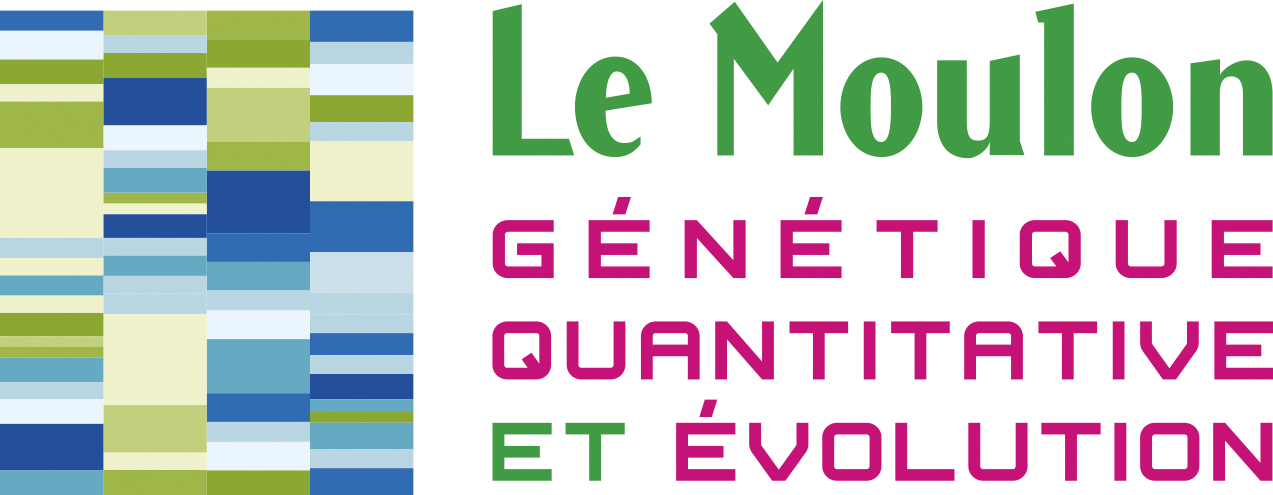
\includegraphics[width=.15\textwidth]{Logo-UMRGV}
\end{center} \vspace{-20pt}
\end{wrapfigure}
\noindent
The Diversity, Evolution and Adaptation of Populations (DEAP) team led by Isabelle Goldringer is part of INRA UMR 0320 Quantitative Genetic and Evolution.
Its work is based on the analysis of the genetic and evolutionary mechanisms underlying evolution and adaptation of crop populations.
DEAP develops strategies for on farm management of crop genetic diversity and
for plant breeding (evolutionary and/or participatory) adated to organic and low input agriculture.
Assessing the benefits of in-field genetic diversity (variety mixtures, populations) and designing
/ breeding optimized mixtures adapted to local conditions are also key research objectives.\\
\url{moulon.inra.fr/index.php/en/team/deap} \\
\noindent
The bioinformatics and informatics facility (ABI, Atelier Bioinformatique et Informatique) provides bioinformatics expertise and IT support. The staff includes 6 experts in system administration, software development or bio-analysis, and develops databases and softwares for proteomics, genetics and genomics. ABI offers hardware resources, scientific programming and consulting for DNA, RNA and protein sequence analysis up to genome-wide scale. ABI works in tight collaboration with the Bioinformatics facilities of University Paris-Sud and INRA, and contributes to the future French Bioinformatics Institute. \\
\url{moulon.inra.fr/index.php/en/tranverse-team} \\


\vfill




\newpage

\tableofcontents

\vfill

\begin{center}
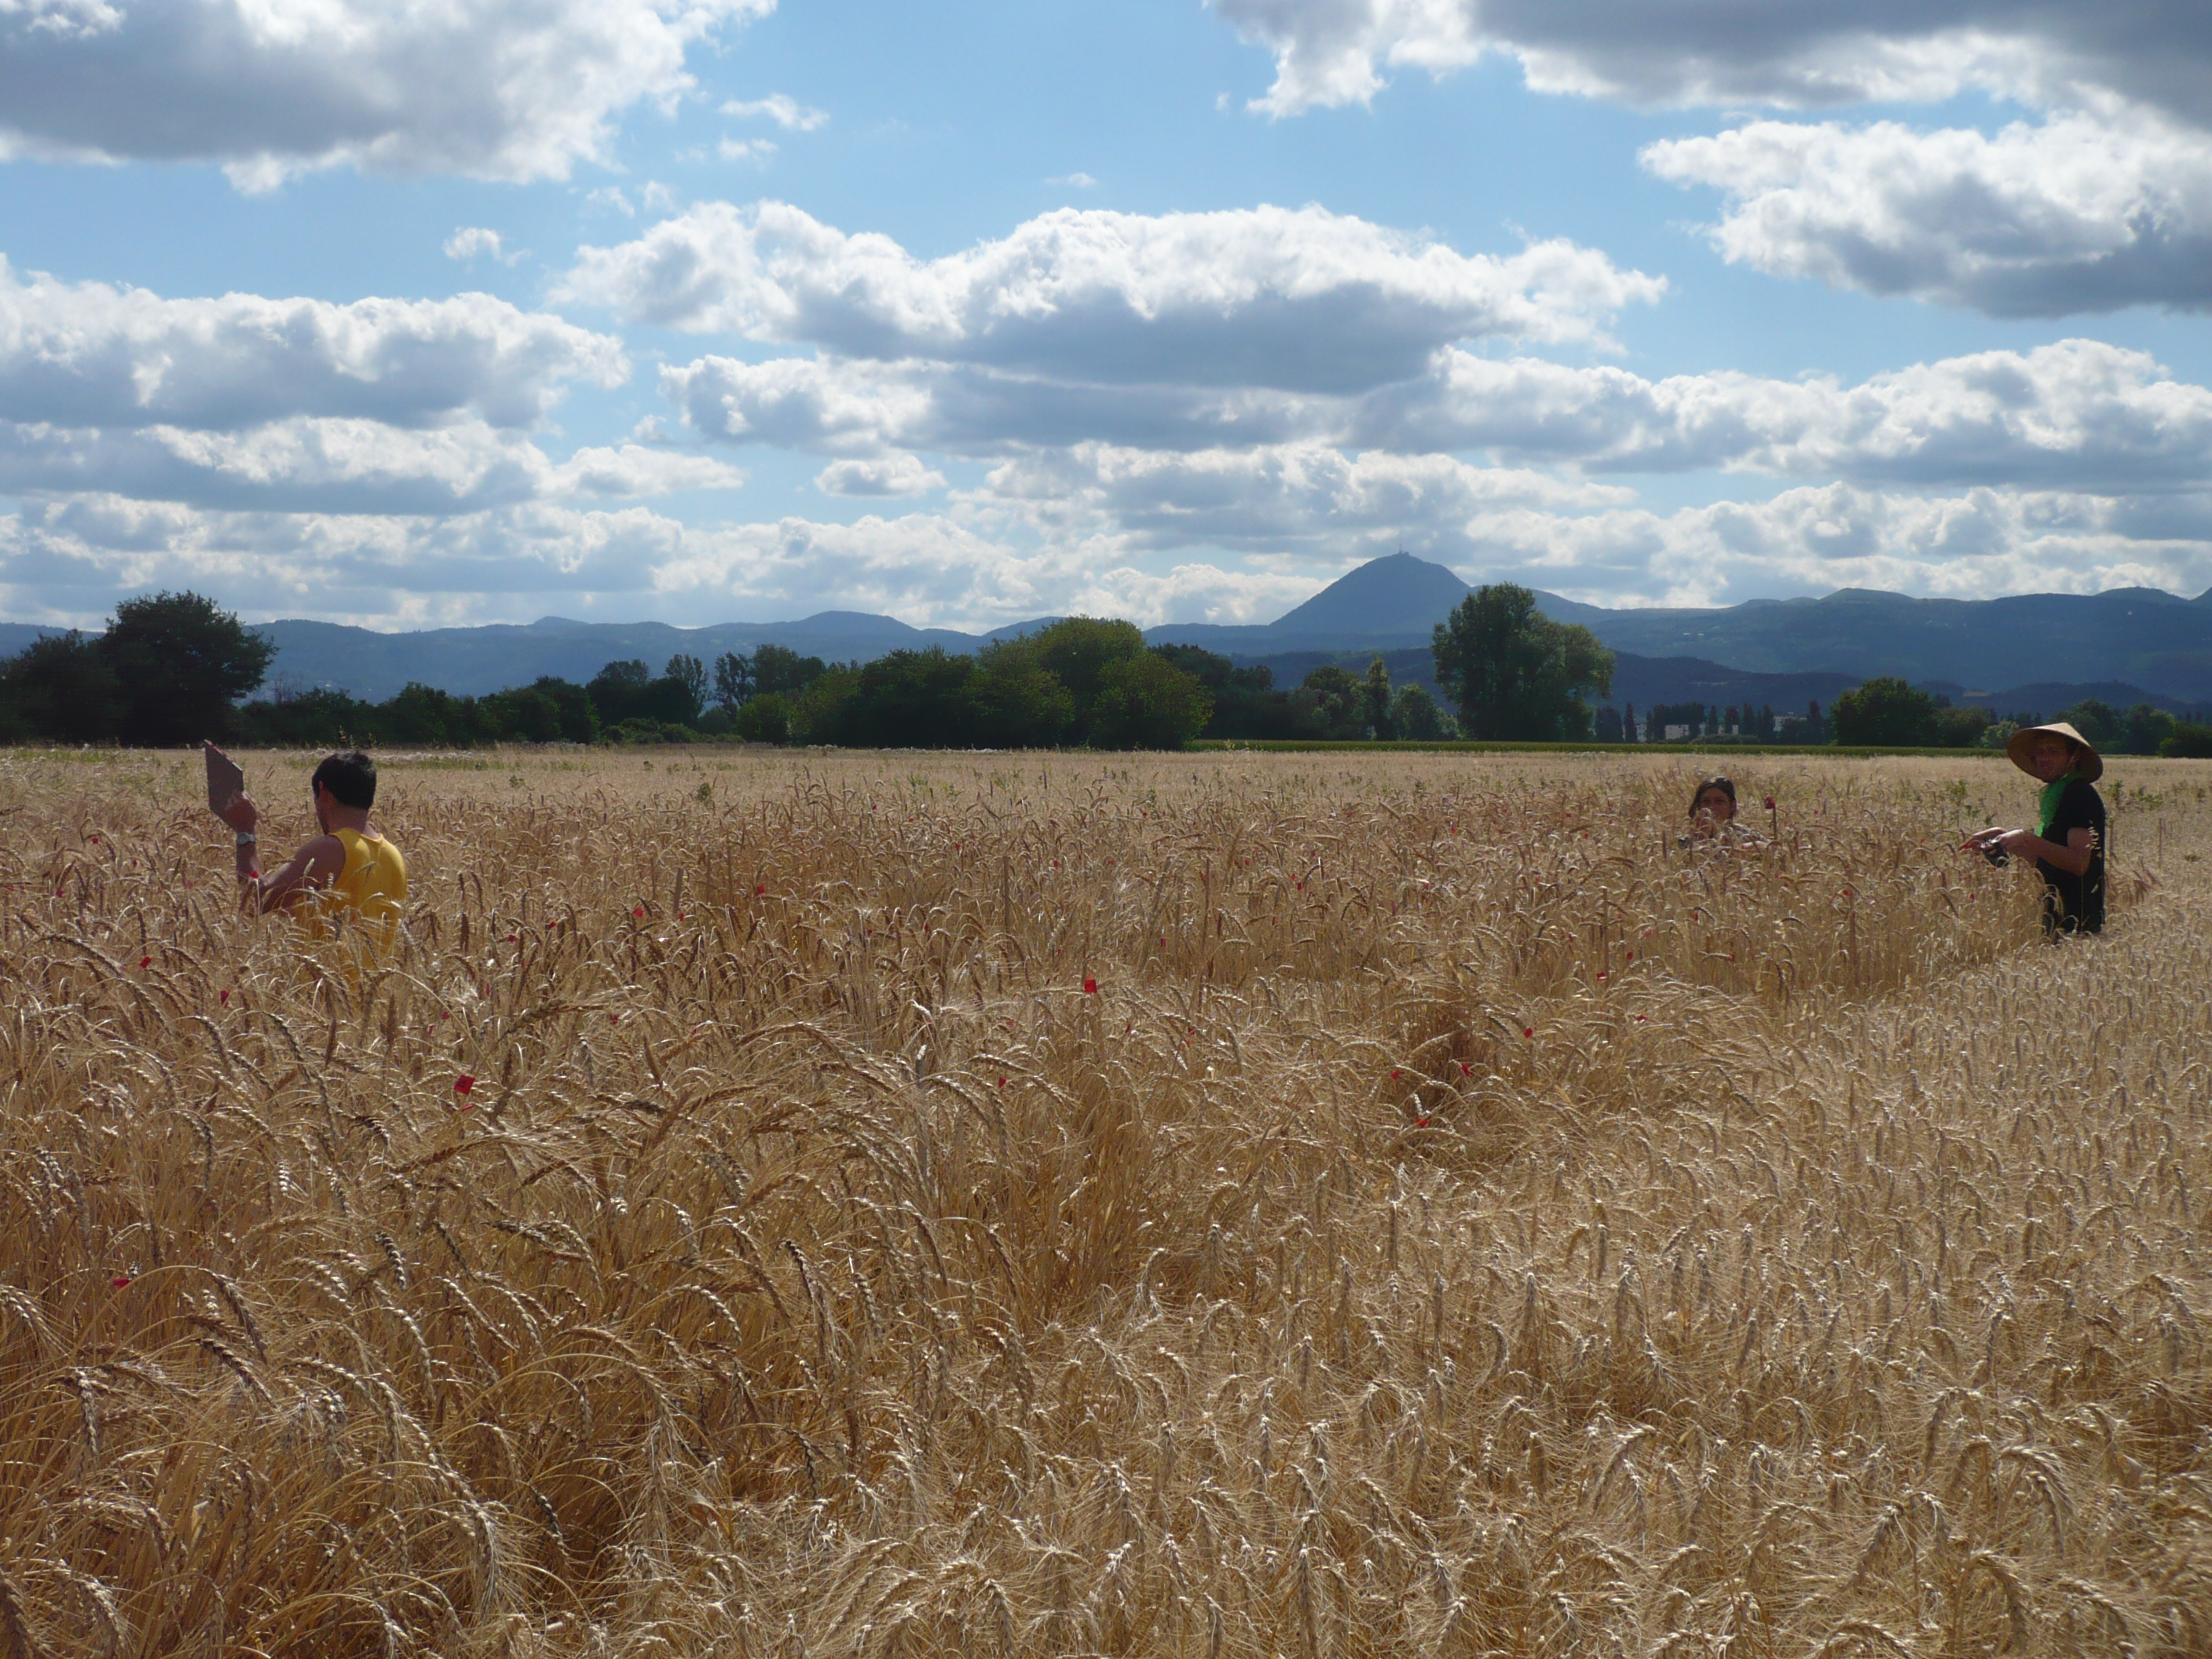
\includegraphics[width=.8\textwidth]{wheat} \\
Wheat trials on farm within our participatory plant breeding programme, summer 2012, Auvergne, France. \\
CC-BY-NC-SA. Pierre Rivière.
\end{center}

\newpage
\pagestyle{plain}


\newpage


\section{Philosophy of \pack}

\subsection{What is \BD?}

Started in 2009, DEAP and ABI teams from INRA Le Moulon developped a data base to store data in a reliable way during research programs dedicated to the study of dynamic management of crop diversity within experimental stations and farmer networks \citep{thomas_gestion_2011}. 

From 2011 to 2013, this data base was migrated to \BDfull~(\BD) and has evolved in a participatory plant breeding program involving INRA Le Moulon and the Réseau Semences Paysannes (RSP) on bread wheat \citep{riviere_methodologie_2014}.

From 2014 to today, farmers organisations' facilitators informed on  their specific needs for their data management, involving other species than bread wheat such as maize, tomatos or trees. Specific developments were performed to fit the farmers organisations' needs. 

\BD~stores information related to (Figure \ref{relation_SL}):
\begin{itemize}
\item network relation betweens \sl
\item data linked to the \sl~and to the relations between \sl
\end{itemize}

\begin{figure}[H]
\begin{center}
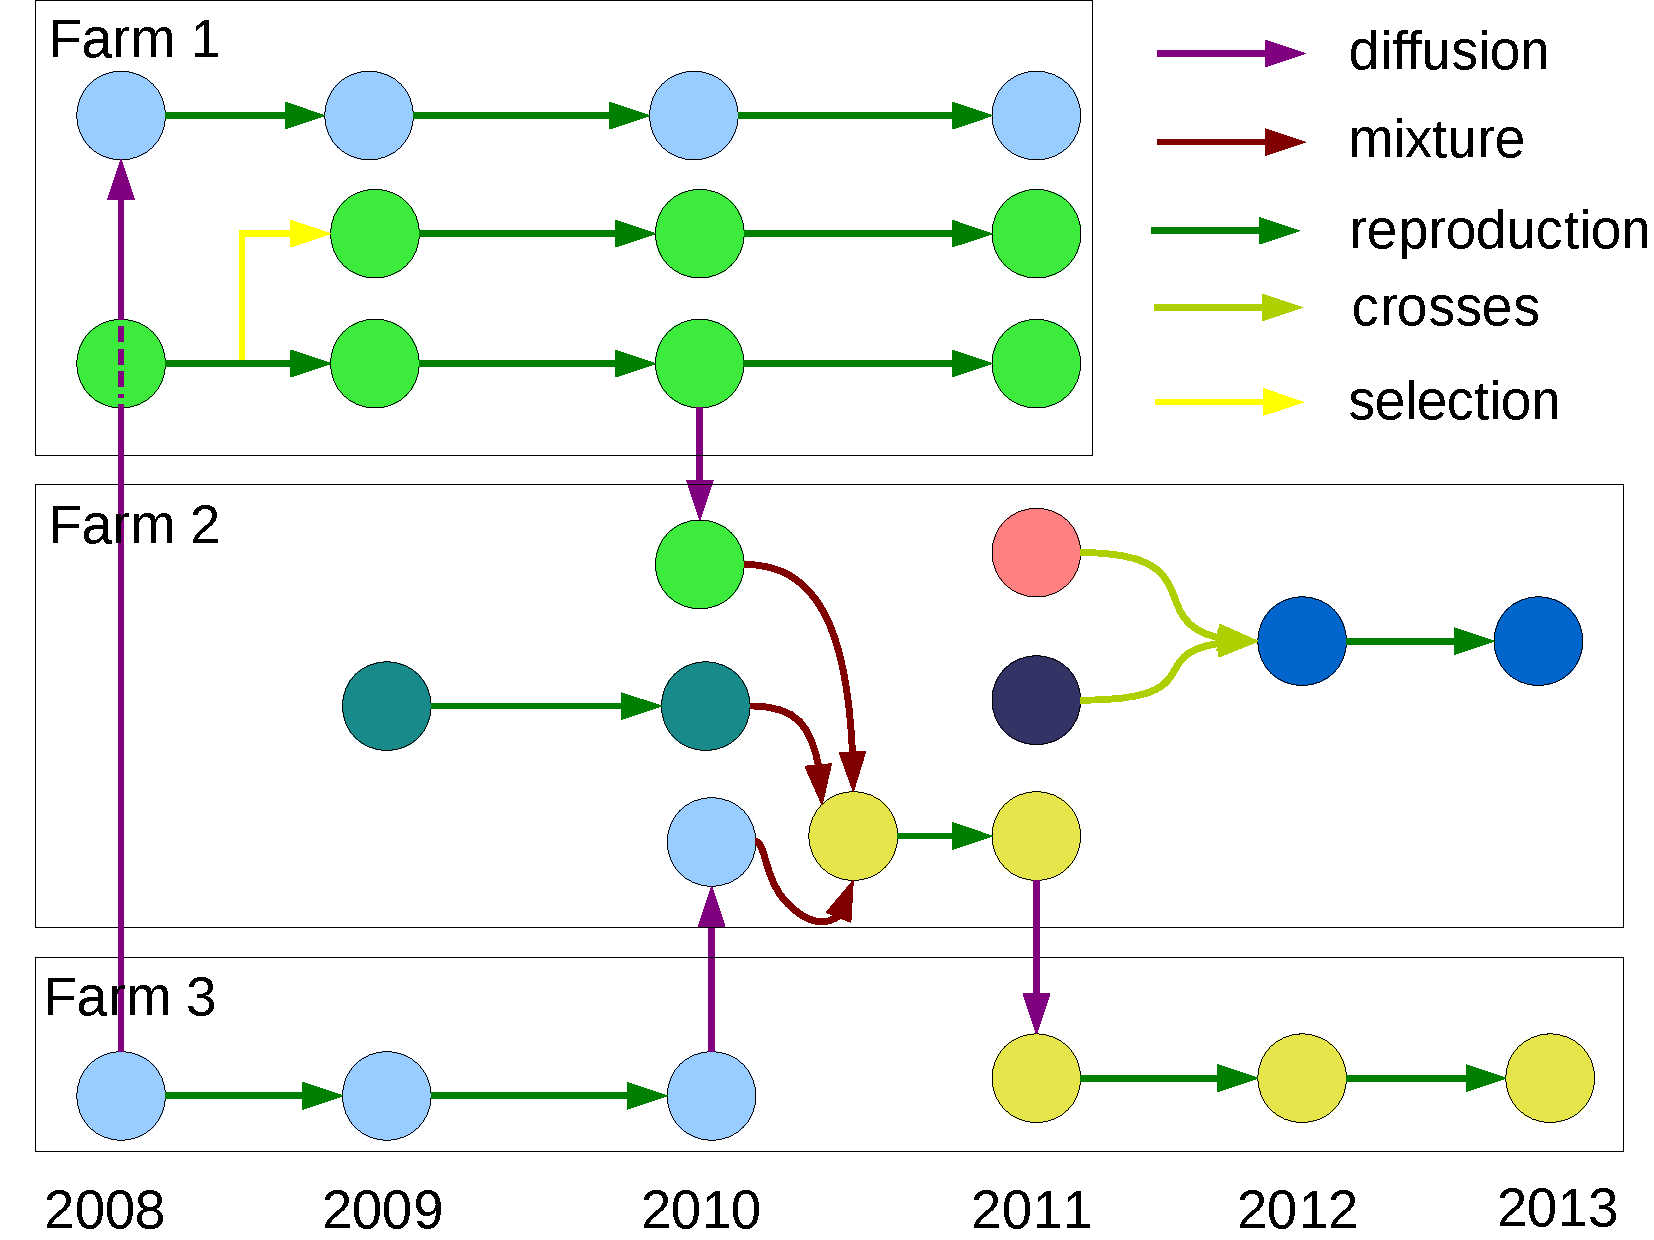
\includegraphics[width=.8\textwidth]{relation_SL_EN}
\caption{
Seed-lots relation in \BD. 
The \sl~are represented by a circle.
The color represents a germplasm (i.e. a variety).
The arrows represent the relations between \sl~(diffusion, mixture, reproduction, crosses and selection).
Data are linked to the \sl~and to the relations between \sl.
}
\label{relation_SL}
\end{center}
\end{figure}

\BD~can be download \href{http://moulon.inra.fr/index.php/en/tranverse-team/atelier-de-bioinformatique/projects/181}{here}.
More information on the history of \BD~and its uses with tutorials can be found on the \href{http://moulon.inra.fr/index.php/en/tranverse-team/atelier-de-bioinformatique/projects/181}{website} \citep{deoliveira_shinemas_2015}.\\

\pack~is an \R~package that analyses outputs from \BD.
It does descriptive analysis, formats data for existing \R~packages to perform statistical analysis as well as compiles results in pdf.


\subsection{Function relations in \pack}

\pack~is divided into three steps (Figure \ref{function_relations}):

\begin{enumerate}
\item Get the data from \BD~with \texttt{get.data}. You may encrypt the data with \texttt{encrypt.data} or translate it with \texttt{translate.data}.
There are two types of data:
\begin{itemize}
\item network relation betweens \sl~(section \ref{network})
\item data linked to the \sl~and to the relations between \sl~(section \ref{data})
\end{itemize}

\item From the data,
	\begin{enumerate}
	\item Get descriptive outputs from the data: plots with \texttt{get.ggplot} or tables with \texttt{get.table}
	\item Get statistical outputs by formating the data with \texttt{format.data} in order to use an existing \R~package~(Up to now the following packages can be used: \texttt{PPBstats})
	\end{enumerate}
\item Get a pdf that compiles the outputs in a pdf document with \texttt{get.pdf} (section \ref{pdf})
\end{enumerate}


\begin{figure}[H]
\begin{center}
%\begin{tikzpicture}[node distance = 2.5cm, auto]
%    % Place nodes
%    \node [block] (data) {get.data};
%    \node [block, below of=data] (plot) {\texttt{get.ggplot}};
%    \node [block, right of=plot] (table) {\texttt{get.table}};
%	\node [block, left of=plot] (format) {\texttt{format.data}};
%	\node [block, below of=format] (pack) {R package};
%	\node [block, below of=pack, right of=pack] (doc) {\texttt{get.doc}};
%
%    % Draw edges
%    \path [line] (data) -- (plot);
%    \path [line] (data) -- (table);
%    \path [line] (plot) -- (doc);
%    \path [line] (table) -- (doc);
%    \path [line,dashed] (data) -- (format);
%    \path [line,dashed] (format) -- (pack);
%    \path [line,dashed] (pack) -- (doc);
%\end{tikzpicture}
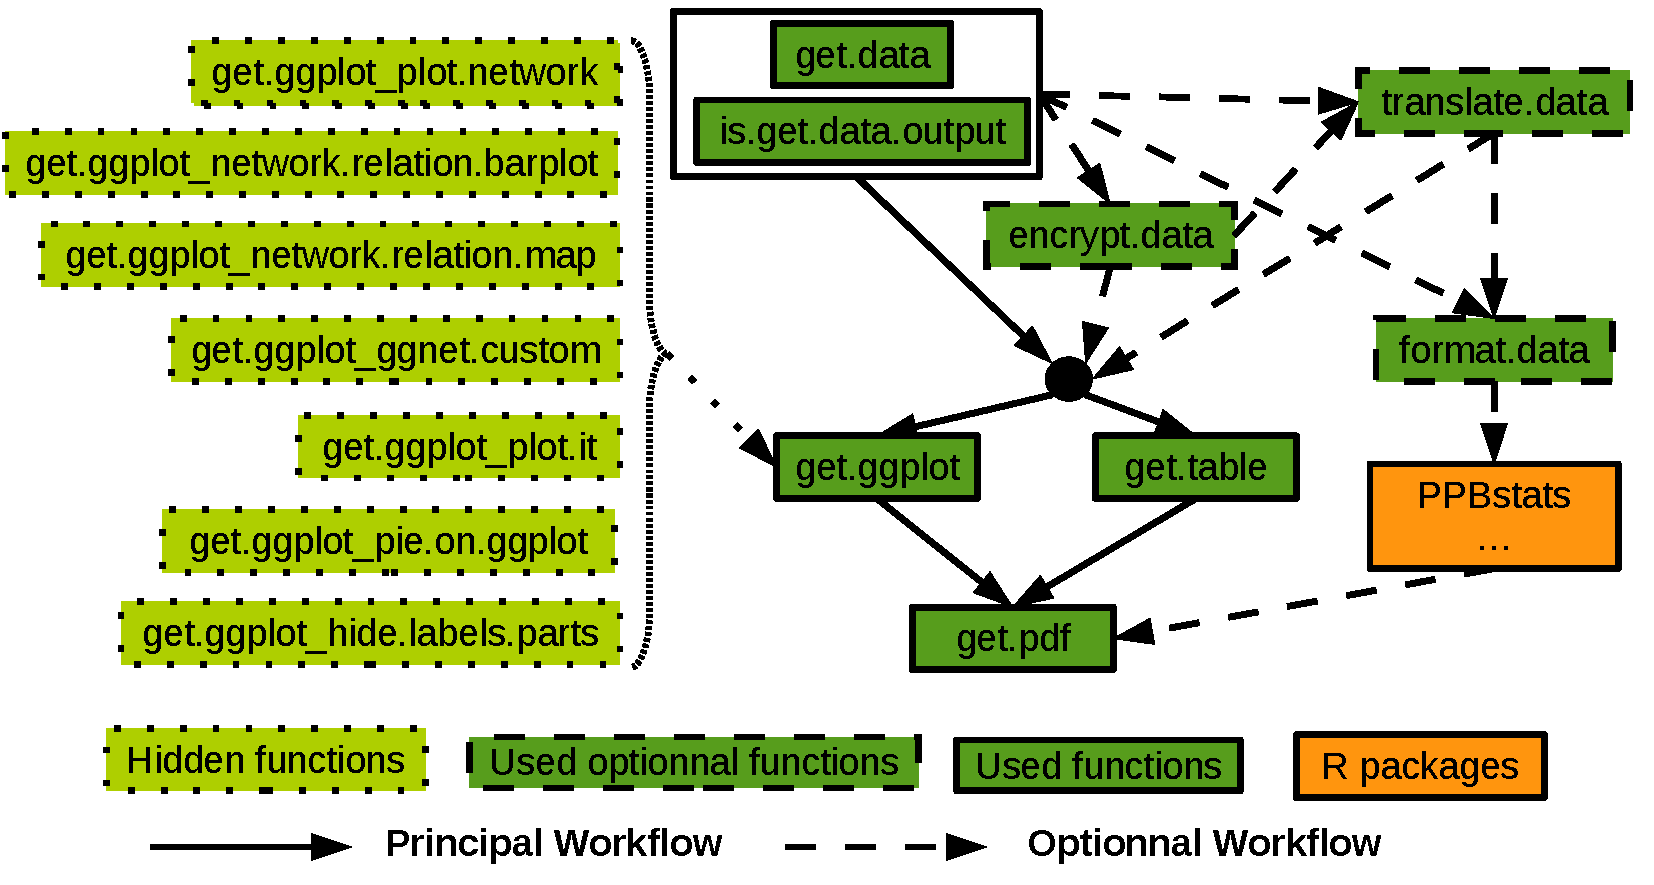
\includegraphics[width=\textwidth]{shinemas2R_function_relations}
\end{center}
\caption{Relations between functions in \pack}
\label{function_relations}
\end{figure}

\texttt{get.ggplot} is based on \texttt{ggplot2} package.
It is therefore easy to custom a plot generated by \texttt{get.ggplot} by adding layers.
More details can be found on the \texttt{ggplot2} documentation website: \url{http://ggplot2.org}.

\subsection{Let’s go!}

To continue, load the package:
\begin{knitrout}
\definecolor{shadecolor}{rgb}{0.969, 0.969, 0.969}\color{fgcolor}\begin{kframe}
\begin{alltt}
\hlkwd{library}\hlstd{(shinemas2R)}
\end{alltt}
\end{kframe}
\end{knitrout}

In this vignette, you can test \pack~without installing \BD.

You can load the data-sets by downloading it:

\begin{knitrout}
\definecolor{shadecolor}{rgb}{0.969, 0.969, 0.969}\color{fgcolor}\begin{kframe}
\begin{alltt}
\hlkwd{system}\hlstd{(}\hlstr{"mkdir data"}\hlstd{)}
\hlkwd{system}\hlstd{(}\hlstr{"cp -r /home/pierre/Documents/geek/R-stats/Rdev/R_package_shinemas2R/shinemas2R_data/*RData ./data"}\hlstd{)}
\end{alltt}
\end{kframe}
\end{knitrout}

and then \texttt{load()} it.


Nevertheless, it may be useful to install \BD~in order to test the \texttt{get.data} function.
The procedure to do so is explained in appendix \ref{install_shinemas}.

For an easier visualisation, all warning messages are not representing (NAs introduced, rows deleted, etc.)


\newpage


\section{Raw information on levels and variables}
\label{raw}

Severals information are stored in \BD.
To get information on raw information and levels and variable, you must use the argument \texttt{query.type} in \texttt{get.data}.
The following table summarize the different possibilities:

\begin{center}
\begin{tabular}{ll}
\hline
\texttt{query.type} & type of information present in \BD \\
\hline
"variable" & variable \\
"person" & person \\
"year" & year \\
"project" & projet \\
"seed.lot" & seed-lots \\
"selection.person" & persons that did intra-varietal mass selection \\
"reproduction.type" & reproduction type \\
"germplasm.type" & germplasm type \\
"germplasm" & germplasm \\
\hline
\end{tabular}
\end{center}

For example,

\begin{knitrout}
\definecolor{shadecolor}{rgb}{0.969, 0.969, 0.969}\color{fgcolor}\begin{kframe}
\begin{alltt}
\hlcom{# person = get.data(}
\hlcom{#	db_user = info_db$db_user, db_host = info_db$db_host,# db infos}
\hlcom{#	db_name = info_db$db_name, db_password = info_db$db_password, # db infos}
\hlcom{#	query.type = "person" # information on person present in SHiNeMaS}
\hlcom{#	)}

\hlkwd{load}\hlstd{(}\hlstr{"data/person.RData"}\hlstd{)}
\hlstd{person}\hlopt{$}\hlstd{data}
\end{alltt}
\begin{verbatim}
##   [1] ""      "ADP"   "AGO"   "ALB"   "ALH"   "ALP"   "ALPO" 
##   [8] "ALR"   "ANB"   "ANW"   "AOV"   "ARB"   "ARC"   "AUD"  
##  [15] "BAM"   "BED"   "BEN"   "BER"   "BRE"   "CAB"   "CAL"  
##  [22] "CEP"   "CER"   "CHD"   "CHH"   "CHP"   "CIG"   "CLB"  
##  [29] "CLF"   "CLM"   "CRP"   "DAC"   "DAL"   "DAT"   "DAV"  
##  [36] "DET"   "DIF"   "DIT"   "DOB"   "EDD"   "ESS"   "EUK"  
##  [43] "FLM"   "FLP"   "FRC"   "FRG"   "FRP"   "FUE"   "GIM"  
##  [50] "GUF"   "GUK"   "HEA"   "HEC"   "HEF"   "HEG"   "HEL"  
##  [57] "HGA"   "HZE"   "I01"   "ICE"   "INE"   "ISG"   "JAB"  
##  [64] "JAR"   "JCM"   "JEF"   "JFB"   "JFM"   "JJG"   "JMC"  
##  [71] "JMM"   "JMR"   "JOP"   "JPB"   "JSG"   "JUB"   "JUD"  
##  [78] "JUM"   "LAG"   "LAH"   "LAU"   "LOD"   "LUD"   "MAF"  
##  [85] "MAI  " "MAS"   "MAT"   "MAV"   "MIR"   "MLN"   "MPH"  
##  [92] "NIS"   "OLM"   "OLR"   "P01"   "P02"   "PAD"   "PAF"  
##  [99] "PAJ"   "PHC"   "PHG"   "PHL"   "PID"   "PIR"   "PIS"  
## [106] "RAB"   "RAL"   "RDR"   "RDZ"   "RIH"   "ROG"   "ROW"  
## [113] "SAC"   "STE"   "STP"   "TEH"   "THG"   "TOA"   "VEN"  
## [120] "VER"   "VIC"   "VIH"   "VJT"   "YVC"   "YVV"  
## attr(,"shinemas2R.object")
## [1] "person"
\end{verbatim}
\end{kframe}
\end{knitrout}



\newpage


\section{Network relations between \sl }
\label{network}

\subsection{Get the data set}

To get the data, use the function \texttt{get.data} with \texttt{query.type = "network"}.

You can set filters to the query with the following argument :

\begin{itemize}
\item \texttt{filter.in} to choose nothing expect \texttt{filter.in}
\item \texttt{filter.out} to choose everything expect \texttt{filter.out}
\end{itemize}

values of \texttt{filter} can be \texttt{germplasm}, \texttt{germplasm.type}, \texttt{year}, \texttt{person}, \texttt{project}, \texttt{\sl}, \texttt{relation} or \texttt{reproduction type}.


It is important to choose if you apply the filter on the \texttt{father} or the \texttt{son} of a relation.
This can be done with the argument \texttt{filter.on}.
Possibles values are \texttt{"father"}, \texttt{"son"} or \texttt{"father-son"}.
It is set by default to \texttt{"father-son"}.

It is possible to get the \texttt{Mdist} square matrix with the number of reproductions that separate two seed-lots since their last common diffusion (argument \texttt{Mdist = TRUE}).
This square matrix can be compared to a differenciation distance. 
It can be put in relation with genetic $F_{st}$ for example \citep{nei_analysis_1973}\footnote{The \R~package \texttt{adegenet} can be used for that.}.


\begin{knitrout}
\definecolor{shadecolor}{rgb}{0.969, 0.969, 0.969}\color{fgcolor}\begin{kframe}
\begin{alltt}
\hlcom{#data_network = get.data(}
\hlcom{#	db_user = info_db$db_user, db_host = info_db$db_host, # db infos}
\hlcom{#	db_name = info_db$db_name, db_password = info_db$db_password, # db infos}
\hlcom{#	query.type = "network", # network query}
\hlcom{#	germplasm.in = "Rouge-du-Roc", # germplasm to keep}
\hlcom{#	filter.on = "father-son", # filter on father AND son}
\hlcom{#	Mdist = TRUE}
\hlcom{#	)}

\hlcom{# 1. Query SHiNeMaS ...}
\hlcom{# 2. Create network matrix ...}
\hlcom{# 3. Link information to vertex and edges ...}
\hlcom{# 4. Get network information on seed-lots ...}
\hlcom{# 5. Get Mdist square matrix ...}

\hlcom{#data_network = encrypt.data(data_network)}
\hlcom{#The key has been written in /home/pierre/key_network_Tue Nov 24 11:52:47 2015.RData}

\hlkwd{load}\hlstd{(}\hlstr{"./data/data_network.RData"}\hlstd{)}
\end{alltt}
\end{kframe}
\end{knitrout}

The function returns a list with:
\begin{itemize}
\item the netwok object
\begin{knitrout}
\definecolor{shadecolor}{rgb}{0.969, 0.969, 0.969}\color{fgcolor}\begin{kframe}
\begin{alltt}
\hlstd{n} \hlkwb{=} \hlstd{data_network}\hlopt{$}\hlstd{data}\hlopt{$}\hlstd{network}
\hlstd{n}
\end{alltt}
\begin{verbatim}
##  Network attributes:
##   vertices = 661 
##   directed = TRUE 
##   hyper = FALSE 
##   loops = FALSE 
##   multiple = FALSE 
##   bipartite = FALSE 
##   total edges= 783 
##     missing edges= 0 
##     non-missing edges= 783 
## 
##  Vertex attribute names: 
##     germplasm germplasm_type germplasm.type person sex vertex.names year 
## 
##  Edge attribute names: 
##     generation relation
\end{verbatim}
\end{kframe}
\end{knitrout}

Note you can convert this object to an \texttt{igraph} object.
This may be useful if you like to use the \texttt{igraph} package.
See \url{http://mbojan.github.io/intergraph/} for more information.

\begin{knitrout}
\definecolor{shadecolor}{rgb}{0.969, 0.969, 0.969}\color{fgcolor}\begin{kframe}
\begin{alltt}
\hlstd{n_igraph} \hlkwb{=} \hlstd{intergraph}\hlopt{::}\hlkwd{asIgraph}\hlstd{(n)}
\hlstd{n_igraph}
\end{alltt}
\begin{verbatim}
## IGRAPH D--- 661 783 -- 
## + attr: germplasm (v/c), germplasm_type (v/c),
## | germplasm.type (v/c), na (v/l), person (v/c), sex (v/c),
## | vertex.names (v/c), year (v/n), generation (e/c), na
## | (e/l), relation (e/c)
## + edges:
##  [1]  2-> 3  3-> 4  3-> 5  4-> 6  5-> 7  6-> 8  8-> 9  7->10  9->11
## [10] 10->12 11->13 12->14 15->16 11->17 11->18 11->19 11->20 11->21
## [19] 11->22 11->23 11->24 11->25 11->26 11->27 11->28 11->29 13->30
## [28] 14->31 11->32 11->33 11->34 11->35 11->36 12->37 11->38 11->39
## [37] 14->40 13->41 13->42 13->43 21->44 21->45 34->46 34->47 34->48
## + ... omitted several edges
\end{verbatim}
\end{kframe}
\end{knitrout}


\item the network.info matrix with information on relation in the network.
\begin{knitrout}
\definecolor{shadecolor}{rgb}{0.969, 0.969, 0.969}\color{fgcolor}\begin{kframe}
\begin{alltt}
\hlkwd{head}\hlstd{(data_network}\hlopt{$}\hlstd{data}\hlopt{$}\hlstd{network.info)}
\end{alltt}
\begin{verbatim}
##                                  sl alt  long   lat diffusion
## 1 germplasm-856_person-67_2002_0001 107  0.42 44.40      <NA>
## 2 germplasm-882_person-67_2002_0001 107  0.42 44.40      <NA>
## 3 germplasm-882_person-43_2002_0001  24 -0.60 47.71   receive
## 4 germplasm-882_person-67_2003_0001 107  0.42 44.40      <NA>
## 5 germplasm-882_person-43_2003_0001  24 -0.60 47.71      <NA>
## 6 germplasm-882_person-67_2004_0001 107  0.42 44.40      <NA>
##   id.diff reproduction mixture selection cross.info     germplasm
## 1    <NA>      harvest    <NA>      <NA>       <NA> germplasm-856
## 2    <NA>  harvest-sow    <NA>      <NA>       <NA> germplasm-882
## 3    3229         <NA>    <NA>      <NA>       <NA> germplasm-882
## 4    <NA>  harvest-sow    <NA>      <NA>       <NA> germplasm-882
## 5    <NA>  harvest-sow    <NA>      <NA>       <NA> germplasm-882
## 6    <NA>  harvest-sow    <NA>      <NA>       <NA> germplasm-882
##      person year
## 1 person-67 2002
## 2 person-67 2002
## 3 person-43 2002
## 4 person-67 2003
## 5 person-43 2003
## 6 person-67 2004
\end{verbatim}
\end{kframe}
\end{knitrout}

\item the \texttt{Mdist} square matrix
\begin{knitrout}
\definecolor{shadecolor}{rgb}{0.969, 0.969, 0.969}\color{fgcolor}\begin{kframe}
\begin{alltt}
\hlkwd{dim}\hlstd{(data_network}\hlopt{$}\hlstd{data}\hlopt{$}\hlstd{Mdist)}
\end{alltt}
\begin{verbatim}
## [1] 627 627
\end{verbatim}
\end{kframe}
\end{knitrout}

\end{itemize}


You may want to fill gaps into you network data set regarding diffusion events (if the information is stored in \BD!).
This may be usefull, regarding a network on one person, to know where do the seed-lots come from.
To do so, use \texttt{fill.diffusion.gap = TRUE}.

\begin{knitrout}
\definecolor{shadecolor}{rgb}{0.969, 0.969, 0.969}\color{fgcolor}\begin{kframe}
\begin{alltt}
\hlcom{#data_network_JAB = get.data(}
\hlcom{#	db_user = info_db$db_user, db_host = info_db$db_host, # db infos}
\hlcom{#	db_name = info_db$db_name, db_password = info_db$db_password,  # db infos}
\hlcom{#	query.type = "network", # network query}
\hlcom{#	person.in = "JAB", # person to keep}
\hlcom{#	filter.on = "father-son" # filter on father AND son}
\hlcom{#	)}

\hlcom{# 1. Query SHiNeMaS ...}
\hlcom{# 2. Create network matrix ...}
\hlcom{# 3. Link information to vertex and edges ...}
\hlcom{# 4. Get network information on seed-lots ...}

\hlcom{#data_network_JAB = encrypt.data(data_network_JAB)}
\hlcom{# The key has been written in /home/pierre/key_network_Tue Nov 24 11:54:53 2015.RData}

\hlkwd{load}\hlstd{(}\hlstr{"./data/data_network_JAB.RData"}\hlstd{)}
\end{alltt}
\end{kframe}
\end{knitrout}

\begin{knitrout}
\definecolor{shadecolor}{rgb}{0.969, 0.969, 0.969}\color{fgcolor}\begin{kframe}
\begin{alltt}
\hlcom{#data_network_JAB_fill_gap = get.data(}
\hlcom{#	db_user = info_db$db_user, db_host = info_db$db_host, # db infos}
\hlcom{#	db_name = info_db$db_name, db_password = info_db$db_password, # db infos}
\hlcom{#	query.type = "network", # network query}
\hlcom{#	person.in = "JAB", # person to keep}
\hlcom{#	filter.on = "father-son", # filter on father AND son}
\hlcom{#	fill.diffusion.gap = TRUE}
\hlcom{#	)}

\hlcom{# 1. Query SHiNeMaS ...}
\hlcom{# 2. Create network matrix ...}
\hlcom{# 2.1. Fill diffusion gaps ...}
\hlcom{# 3. Link information to vertex and edges ...}
\hlcom{# 4. Get network information on seed-lots ...}

\hlcom{#data_network_JAB_fill_gap = encrypt.data(data_network_JAB_fill_gap)}
\hlcom{# The key has been written in /home/pierre/key_network_Tue Nov 24 11:55:53 2015.RData}

\hlkwd{load}\hlstd{(}\hlstr{"./data/data_network_JAB_fill_gap.RData"}\hlstd{)}
\end{alltt}
\end{kframe}
\end{knitrout}


\subsection{Get the ggplots}

Once, you have got the data, you can do plots with the function \texttt{get.ggplot}.


\begin{knitrout}
\definecolor{shadecolor}{rgb}{0.969, 0.969, 0.969}\color{fgcolor}\begin{kframe}
\begin{alltt}
\hlstd{default_network_ggplot} \hlkwb{=} \hlkwd{get.ggplot}\hlstd{(data_network)}
\end{alltt}


{\ttfamily\noindent\itshape\color{messagecolor}{\#\# As ggplot.type is NULL, ggplot.type is set to network-network, network-reproduction-harvested, network-reproduction-positive-inter-selected, network-reproduction-positive-inter-selected, network-reproduction-negative-inter-selected, network-reproduction-crossed, network-diffusion-sent, network-diffusion-received, network-diffusion-relation, network-mixture, network-positive-intra-selected\\\#\# As ggplot.display is NULL, ggplot.display is set to c("{}barplot"{}, "{}map"{}). Note that for ggplot.type == "{}network-diffusion-relation"{}, ggplot.display is set to "{}map"{} \\\#\# As x.axis and in.col are NULL, all the combinaisons of x.axis and in.col are done for barplot.}}\begin{verbatim}
## [1] "A METTRE A JOUR QUAND ON AURA EVENT YEAR"
## [1] "A METTRE A JOUR QUAND ON AURA EVENT YEAR"
\end{verbatim}
\end{kframe}
\end{knitrout}

By default, all the possibles plots or maps are done.

\begin{knitrout}
\definecolor{shadecolor}{rgb}{0.969, 0.969, 0.969}\color{fgcolor}\begin{kframe}
\begin{alltt}
\hlkwd{names}\hlstd{(default_network_ggplot)}
\end{alltt}
\begin{verbatim}
##  [1] "network-network"                             
##  [2] "network-reproduction-harvested"              
##  [3] "network-reproduction-positive-inter-selected"
##  [4] "network-reproduction-negative-inter-selected"
##  [5] "network-diffusion-sent"                      
##  [6] "network-diffusion-received"                  
##  [7] "network-diffusion-relation"                  
##  [8] "network-mixture"                             
##  [9] "network-positive-intra-selected"             
## [10] "network-reproduction-crossed"
\end{verbatim}
\end{kframe}
\end{knitrout}

It is possible to get only one plot by choosing one of the above name with the argument \texttt{ggplot.type}.
Each \texttt{ggplot.type} with default and custom arguments are explained in the following sub-sections.

\subsubsection{\texttt{ggplot.type = "network-network"}}

\paragraph{Default arguments}

By default, the following network is display:

\begin{knitrout}
\definecolor{shadecolor}{rgb}{0.969, 0.969, 0.969}\color{fgcolor}\begin{kframe}
\begin{alltt}
\hlstd{p_net_RdR} \hlkwb{=} \hlstd{default_network_ggplot}\hlopt{$}\hlstr{"network-network"}
\hlstd{p_net_RdR}
\end{alltt}
\end{kframe}

{\centering \includegraphics[width=\maxwidth]{figures/shinemas2R_unnamed-chunk-20-1} 

}



\end{knitrout}


Regarding the argument \texttt{fill.diffusion.gap} in the function \texttt{get.data}:

\begin{knitrout}
\definecolor{shadecolor}{rgb}{0.969, 0.969, 0.969}\color{fgcolor}\begin{kframe}
\begin{alltt}
\hlstd{p_JAB} \hlkwb{=} \hlkwd{get.ggplot}\hlstd{(}
        \hlstd{data_network_JAB,}
        \hlkwc{ggplot.type} \hlstd{=} \hlstr{"network-network"}\hlstd{,}
        \hlkwc{vertex.color} \hlstd{=} \hlstr{"person"}
        \hlstd{)}
\hlstd{p_JAB} \hlkwb{=} \hlstd{p_JAB}\hlopt{$}\hlstd{`network-network`}

\hlstd{p_JAB_fill_gap} \hlkwb{=} \hlkwd{get.ggplot}\hlstd{(}
        \hlstd{data_network_JAB_fill_gap,}
        \hlkwc{ggplot.type} \hlstd{=} \hlstr{"network-network"}\hlstd{,}
        \hlkwc{vertex.color} \hlstd{=} \hlstr{"person"}
        \hlstd{)}
\hlstd{p_JAB_fill_gap} \hlkwb{=} \hlstd{p_JAB_fill_gap}\hlopt{$}\hlstd{`network-network`}
\end{alltt}
\end{kframe}
\end{knitrout}

We can see that extra information are added to know from where come the seed-lots.

\begin{center}
\begin{tabular}{cc}
\texttt{p\_JAB} & \texttt{p\_JAB\_fill\_gap} \\
\begin{knitrout}
\definecolor{shadecolor}{rgb}{0.969, 0.969, 0.969}\color{fgcolor}

{\centering \includegraphics[width=.5\textwidth]{figures/shinemas2R_unnamed-chunk-22-1} 

}



\end{knitrout}
&
\begin{knitrout}
\definecolor{shadecolor}{rgb}{0.969, 0.969, 0.969}\color{fgcolor}

{\centering 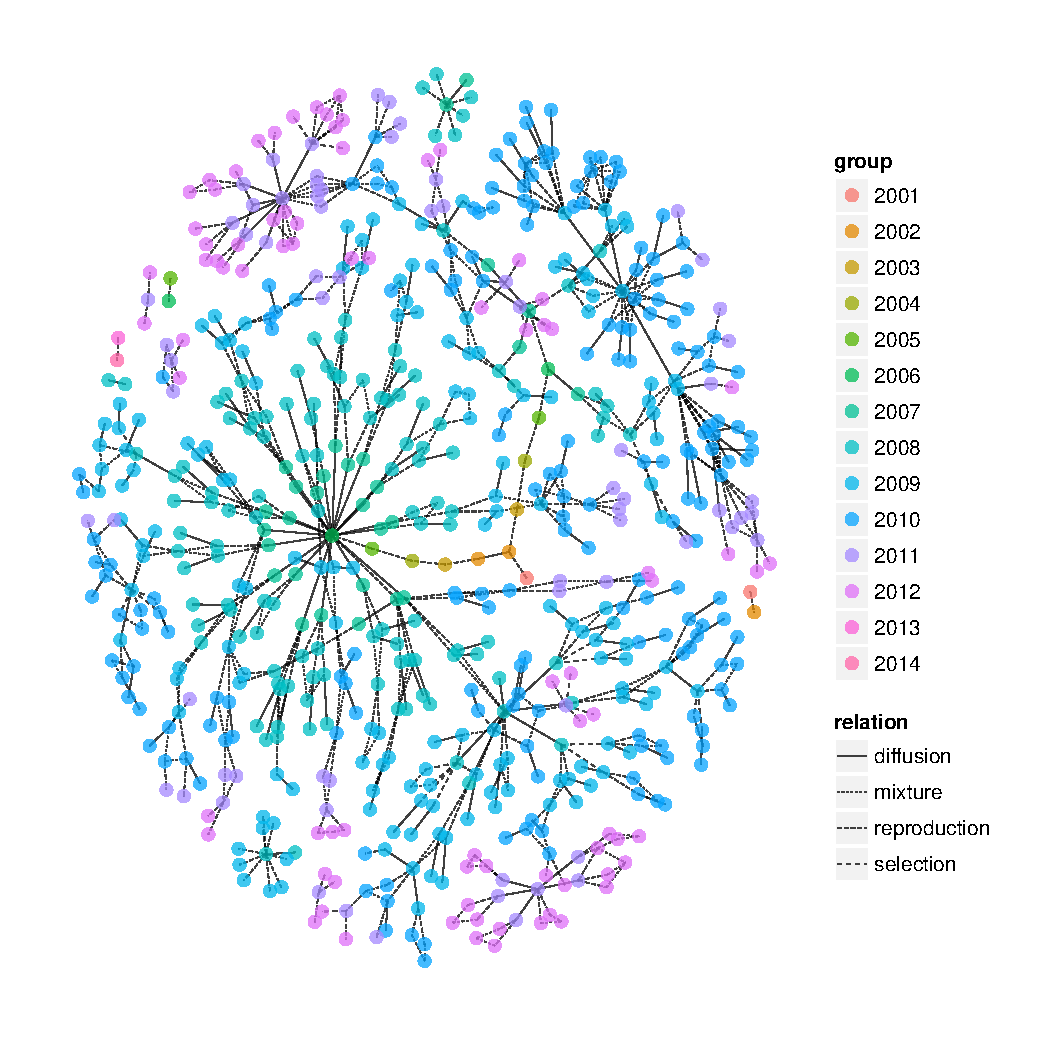
\includegraphics[width=.5\textwidth]{figures/shinemas2R_unnamed-chunk-23-1} 

}



\end{knitrout}
\\
\end{tabular}
\end{center}



\paragraph{Custom arguments}

It is possible to tune the following arguments (Table \ref{custom.network}):


\begin{center}
\begin{table}[H]
\begin{tabular}{ p{.2\textwidth} p{.15\textwidth} p{.6\textwidth} }
\hline
\texttt{argument} & \texttt{default value} & description \\
\hline

\texttt{filter.on} & \texttt{"father-son"} & it chooses on which seed-lots the filters is applied: \texttt{"son"}, \texttt{"father"} or \texttt{"father-son"}. \\

\texttt{vertex.size} & \texttt{3} &  size of the vertex \\

\texttt{vertex.color} & \texttt{"year"} & color of the vertex. 
It can be chosen according to  \texttt{"person"}, \texttt{"germplasm"} or \texttt{"year"}. 
If \texttt{NULL}, it is in black. \\

\texttt{organise.sl} & \texttt{FALSE} & organise seed-lots for an easier visualisation \\

\texttt{hide.labels.parts} & \texttt{"all"} & parts of the label hidden: \texttt{"germplasm"}, \texttt{"person"}, \texttt{"year"}, \texttt{"person:germplasm"}, \texttt{"year:germplasm"}, \texttt{"person:year"}, \texttt{"all"}. 
\texttt{"all"} means that no labels are dispayed. 
If \texttt{NULL} labels are displayed. Labels are based on seed-lots names under the form \texttt{germplasm\_year\_person\_digit}.
For easier visualisation, Digit is never display unless you choose \texttt{NULL}.
\\

\texttt{labels.sex} & \texttt{TRUE} & if \texttt{TRUE}, display the sex of the seed-lot if it has been used in a cross. Nothing is displayed if hide.labels.parts = \texttt{"all"}. \\

\texttt{labels.generation} & \texttt{TRUE} & if TRUE, display generation for each reproduction \\

\texttt{labels.size} & \texttt{3} & size of the labels \\
\hline
\end{tabular}
\caption{Possible arguments to custom arguments regarding network.}
\label{custom.network}
\end{table}
\end{center}


For example,

\begin{knitrout}
\definecolor{shadecolor}{rgb}{0.969, 0.969, 0.969}\color{fgcolor}\begin{kframe}
\begin{alltt}
\hlkwd{get.ggplot}\hlstd{(}
        \hlstd{data_network,}
        \hlkwc{ggplot.type} \hlstd{=} \hlstr{"network-network"}\hlstd{,}
        \hlkwc{organise.sl} \hlstd{=} \hlnum{TRUE}\hlstd{,}
        \hlkwc{hide.labels.parts} \hlstd{=} \hlstr{"year:germplasm"}\hlstd{,}
        \hlkwc{vertex.color} \hlstd{=} \hlstr{"year"}
        \hlstd{)}
\end{alltt}
\begin{verbatim}
## $`network-network`
\end{verbatim}
\end{kframe}


{\centering \includegraphics[width=\maxwidth]{figures/shinemas2R_unnamed-chunk-24-1} 

}



\end{knitrout}

\subsubsection{\texttt{ggplot.type = "network-reproduction-harvested"}}


\texttt{ggplot.type = "network-reproduction-harvested"} corresponds to seed-lots that have been harvested after a reproduction.


Two plots are possibles regarding \texttt{ggplot.display}.

\begin{center}
\begin{tabular}{ p{.2\textwidth} p{.15\textwidth} p{.6\textwidth} }
\hline
argument & default value & description \\
\hline
\texttt{ggplot.display} & \texttt{NULL} & \texttt{"barplot"} or  \texttt{"map"}.
It can be a vector of several elements i.e. \texttt{c("barplot", "map")}. 
\texttt{NULL} by default: both are done. \\
\hline
\end{tabular}
\end{center}


\paragraph{\texttt{ggplot.display = barplot}}

For \texttt{ggplot.display = "barplot"}, you may chose what you want in the x axis (\texttt{x.axis} argument) and in color (\texttt{in.col} argument).
The possible values for \texttt{x.axis} and \texttt{in.col} are: \texttt{germplasm}, \texttt{year}, \texttt{person}.
By default all combinaisons of \texttt{x.axis} and \texttt{in.col} are done with default argument settings.
The name of the plot is under the form \texttt{x.axis}-\texttt{in.col}.


\begin{itemize}

\item Default arguments

\begin{knitrout}
\definecolor{shadecolor}{rgb}{0.969, 0.969, 0.969}\color{fgcolor}\begin{kframe}
\begin{alltt}
\hlstd{p_slh} \hlkwb{=} \hlstd{default_network_ggplot}\hlopt{$}\hlstd{`network-reproduction-harvested`}\hlopt{$}\hlstd{barplot}
\hlstd{p1_slh} \hlkwb{=} \hlstd{p_slh}\hlopt{$}\hlstd{`germplasm-year`}\hlopt{$}\hlstd{`x.axis-1|in.col-1`}
\hlstd{p2_slh} \hlkwb{=} \hlstd{p_slh}\hlopt{$}\hlstd{`germplasm-person`}\hlopt{$}\hlstd{`x.axis-1|in.col-1`}
\hlstd{p3_slh} \hlkwb{=} \hlstd{p_slh}\hlopt{$}\hlstd{`person-year`}\hlopt{$}\hlstd{`x.axis-1|in.col-1`}
\hlstd{p4_slh} \hlkwb{=} \hlstd{p_slh}\hlopt{$}\hlstd{`person-germplasm`}\hlopt{$}\hlstd{`x.axis-1|in.col-1`}
\hlstd{p5_slh} \hlkwb{=} \hlstd{p_slh}\hlopt{$}\hlstd{`year-person`}\hlopt{$}\hlstd{`x.axis-1|in.col-1`}
\hlstd{p6_slh} \hlkwb{=} \hlstd{p_slh}\hlopt{$}\hlstd{`year-germplasm`}\hlopt{$}\hlstd{`x.axis-1|in.col-1`}
\end{alltt}
\end{kframe}
\end{knitrout}

with

\begin{center}
\begin{tabular}{ccc}
\hline
plot & \texttt{x.axis} & \texttt{in.col} \\
\hline
\texttt{p1\_slh} & \texttt{"germplasm"} & \texttt{"year"} \\
\texttt{p2\_slh} & \texttt{"germplasm"} & \texttt{"person"} \\
\texttt{p3\_slh} & \texttt{"person"} & \texttt{"year"} \\
\texttt{p4\_slh} & \texttt{"person"} & \texttt{"germplasm"} \\
\texttt{p5\_slh} & \texttt{"year"} & \texttt{"person"} \\
\texttt{p6\_slh} & \texttt{"year"} & \texttt{"germplasm"} \\
\hline
\end{tabular}
\end{center}


\begin{center}
\begin{tabular}{cc}
\texttt{p1\_slh} & \texttt{p2\_slh} \\
\begin{knitrout}
\definecolor{shadecolor}{rgb}{0.969, 0.969, 0.969}\color{fgcolor}

{\centering 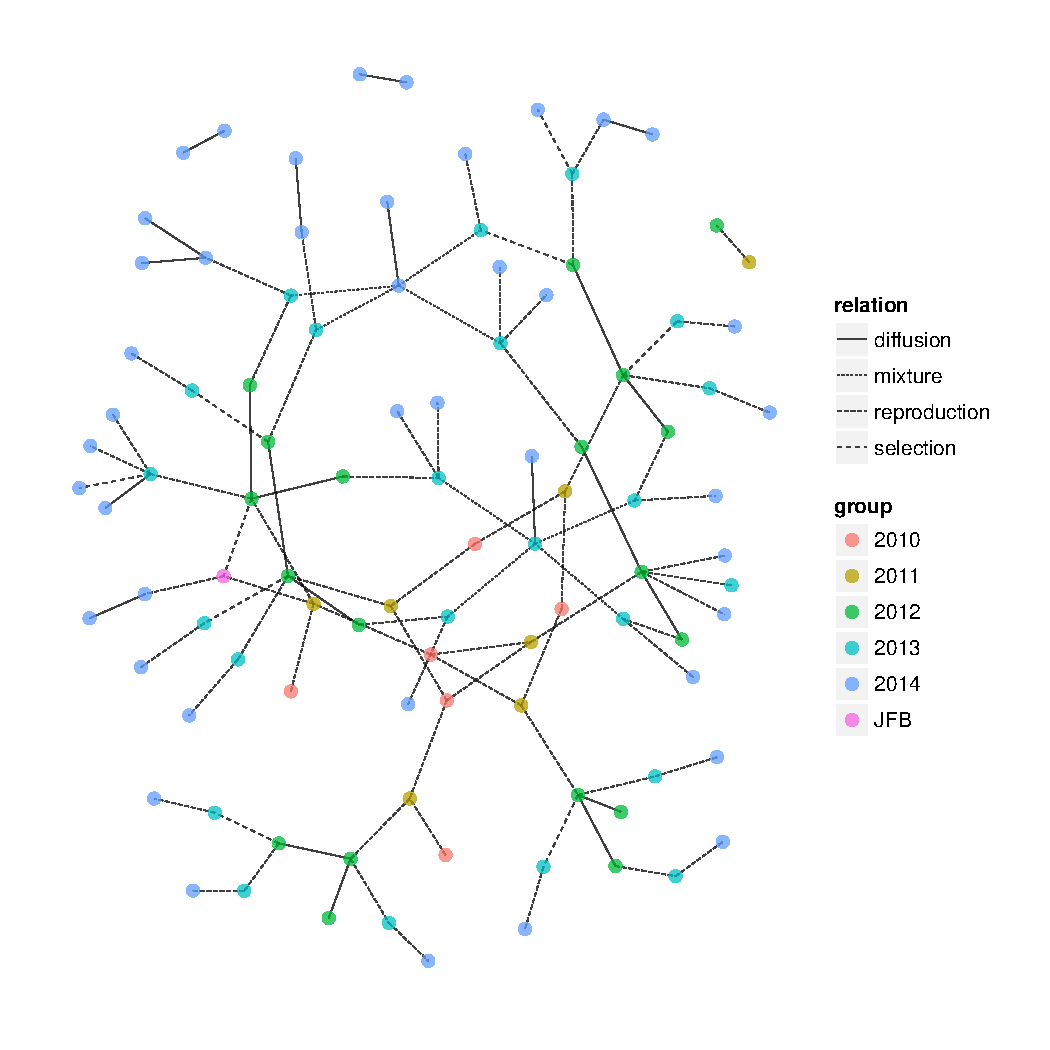
\includegraphics[width=.4\textwidth]{figures/shinemas2R_unnamed-chunk-26-1} 

}



\end{knitrout}
&
\begin{knitrout}
\definecolor{shadecolor}{rgb}{0.969, 0.969, 0.969}\color{fgcolor}

{\centering 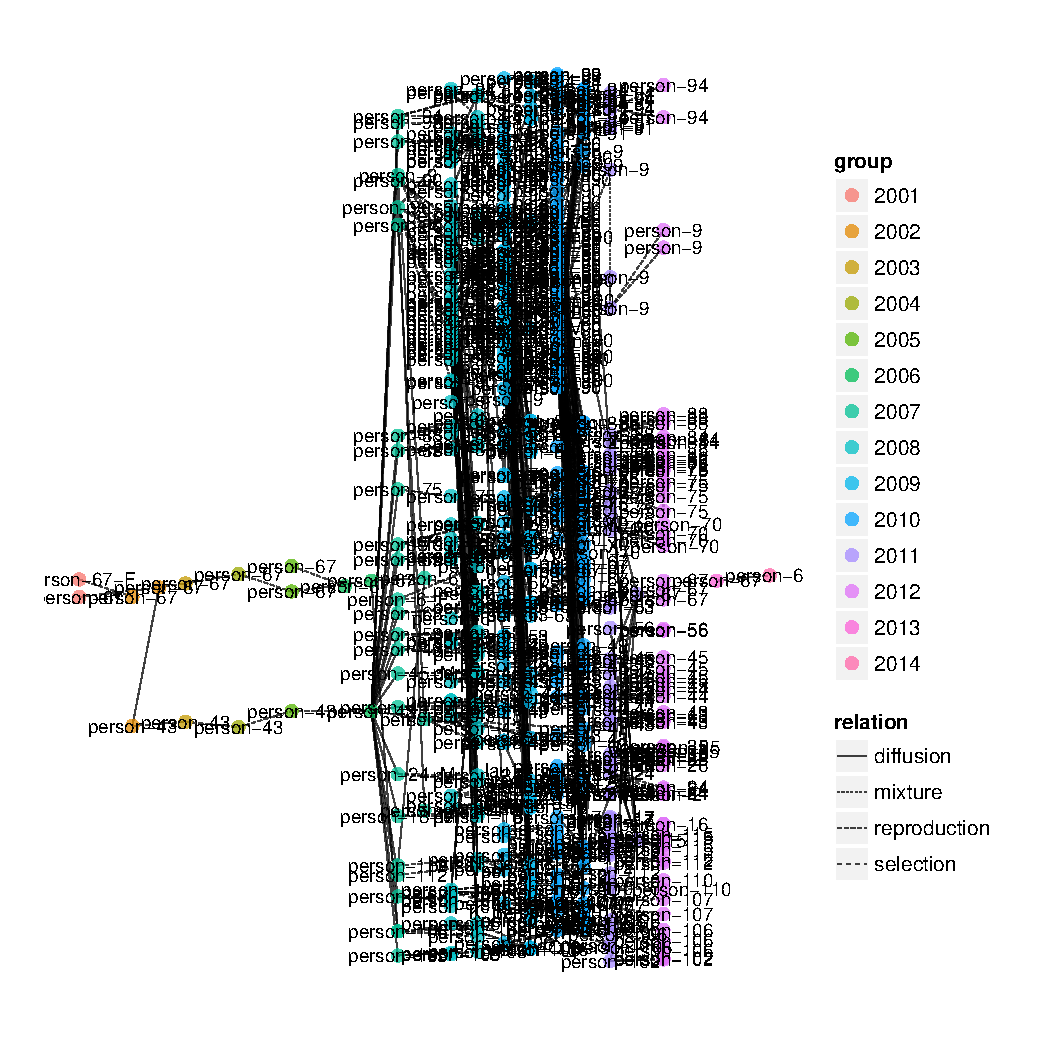
\includegraphics[width=.4\textwidth]{figures/shinemas2R_unnamed-chunk-27-1} 

}



\end{knitrout}
\\
\texttt{p3\_slh} & \texttt{p4\_slh} \\
\begin{knitrout}
\definecolor{shadecolor}{rgb}{0.969, 0.969, 0.969}\color{fgcolor}

{\centering 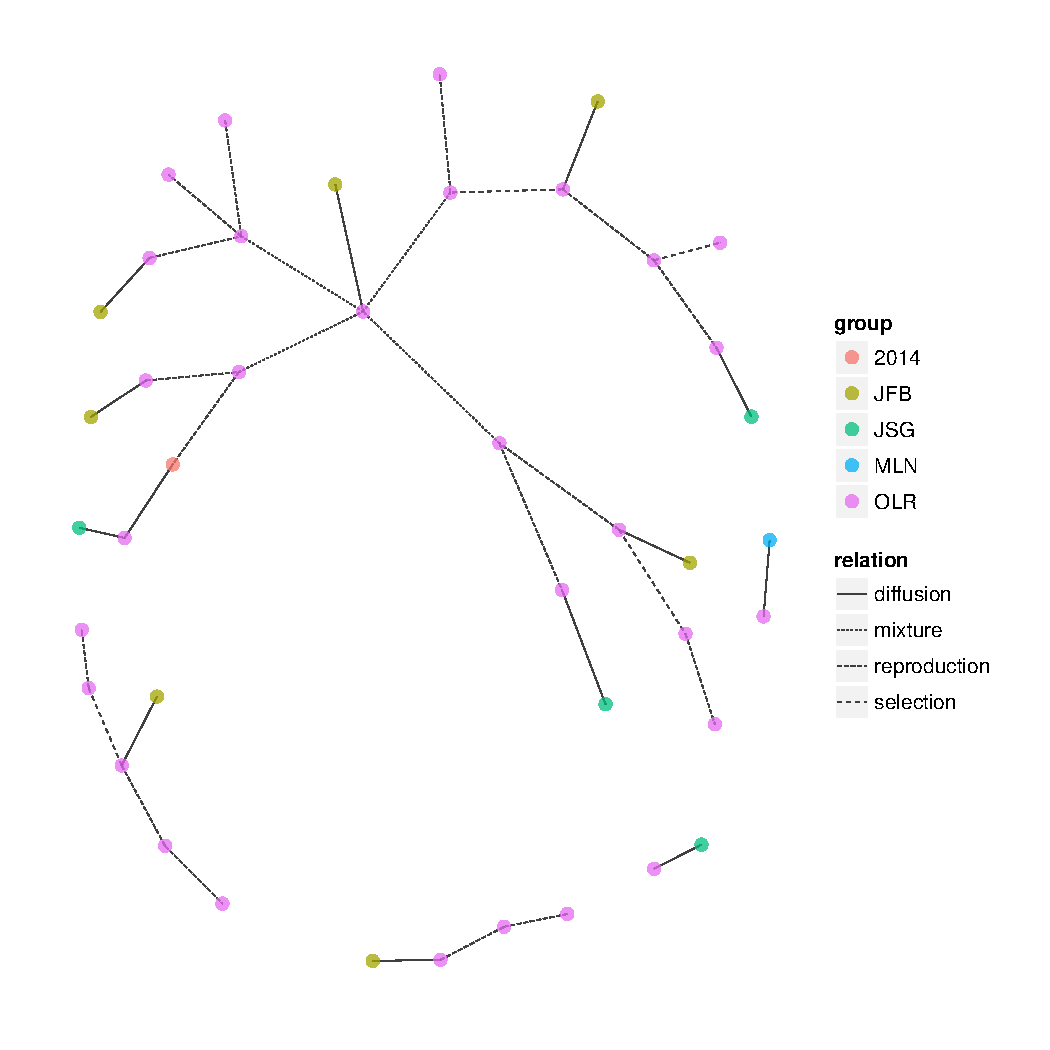
\includegraphics[width=.4\textwidth]{figures/shinemas2R_unnamed-chunk-28-1} 

}



\end{knitrout}
&
\begin{knitrout}
\definecolor{shadecolor}{rgb}{0.969, 0.969, 0.969}\color{fgcolor}

{\centering 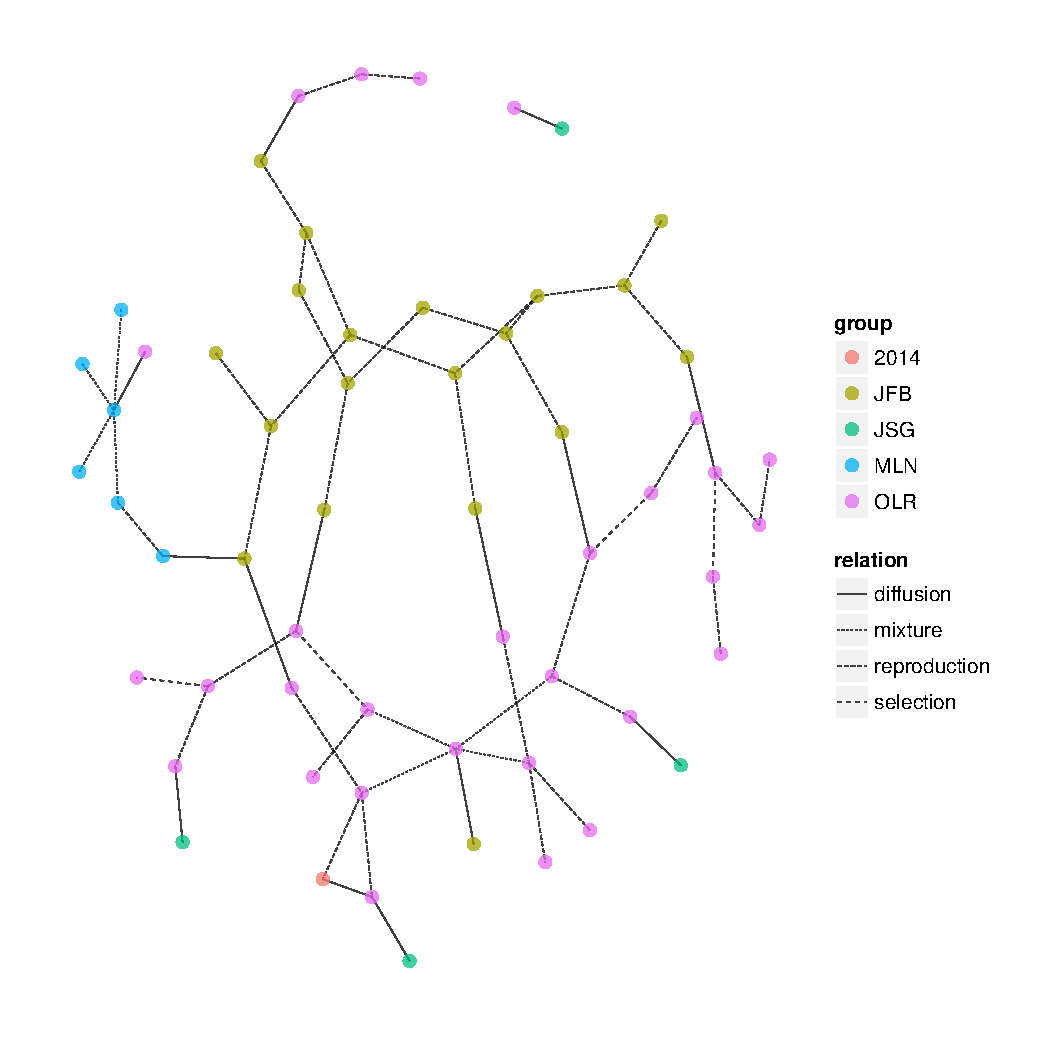
\includegraphics[width=.4\textwidth]{figures/shinemas2R_unnamed-chunk-29-1} 

}



\end{knitrout}
\\
\texttt{p5\_slh} & \texttt{p6\_slh} \\
\begin{knitrout}
\definecolor{shadecolor}{rgb}{0.969, 0.969, 0.969}\color{fgcolor}

{\centering 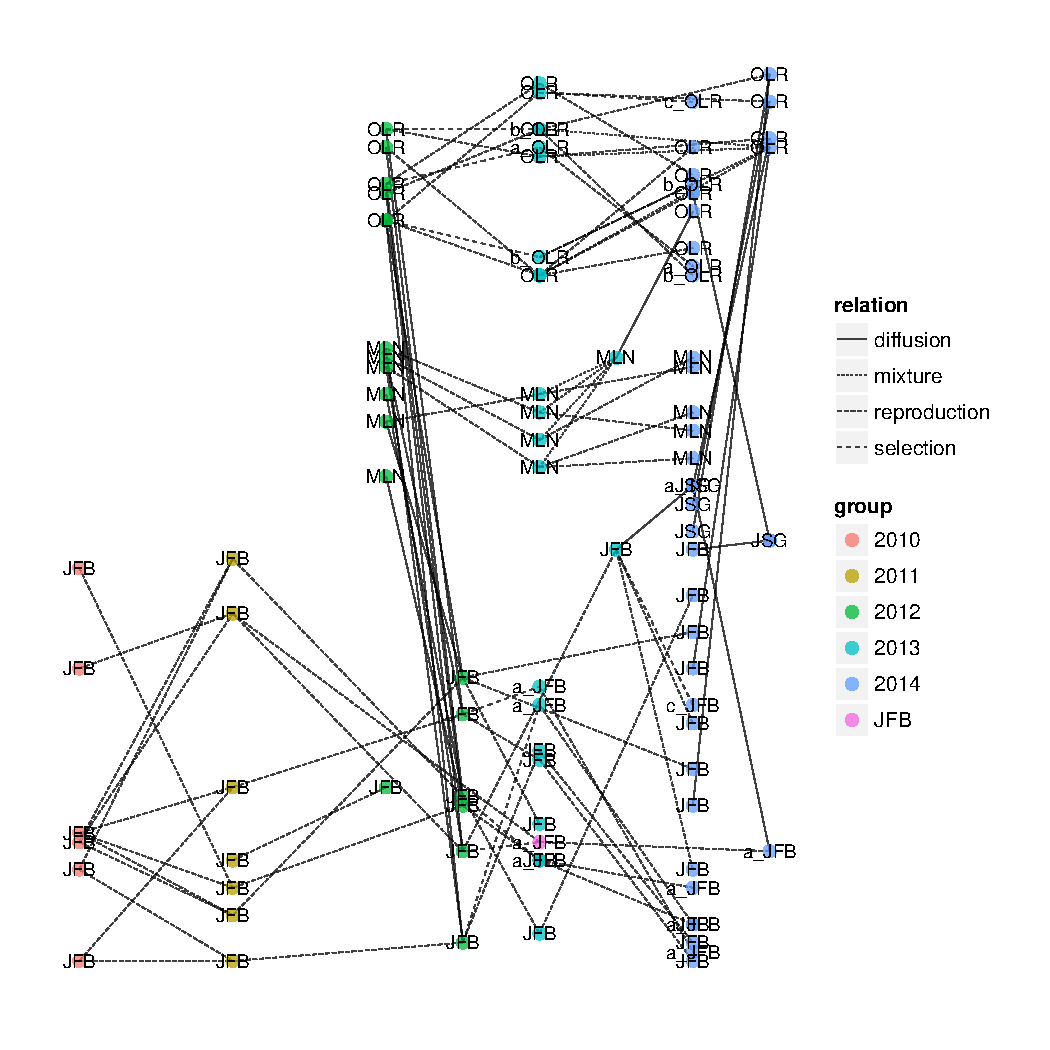
\includegraphics[width=.4\textwidth]{figures/shinemas2R_unnamed-chunk-30-1} 

}



\end{knitrout}
&
\begin{knitrout}
\definecolor{shadecolor}{rgb}{0.969, 0.969, 0.969}\color{fgcolor}

{\centering 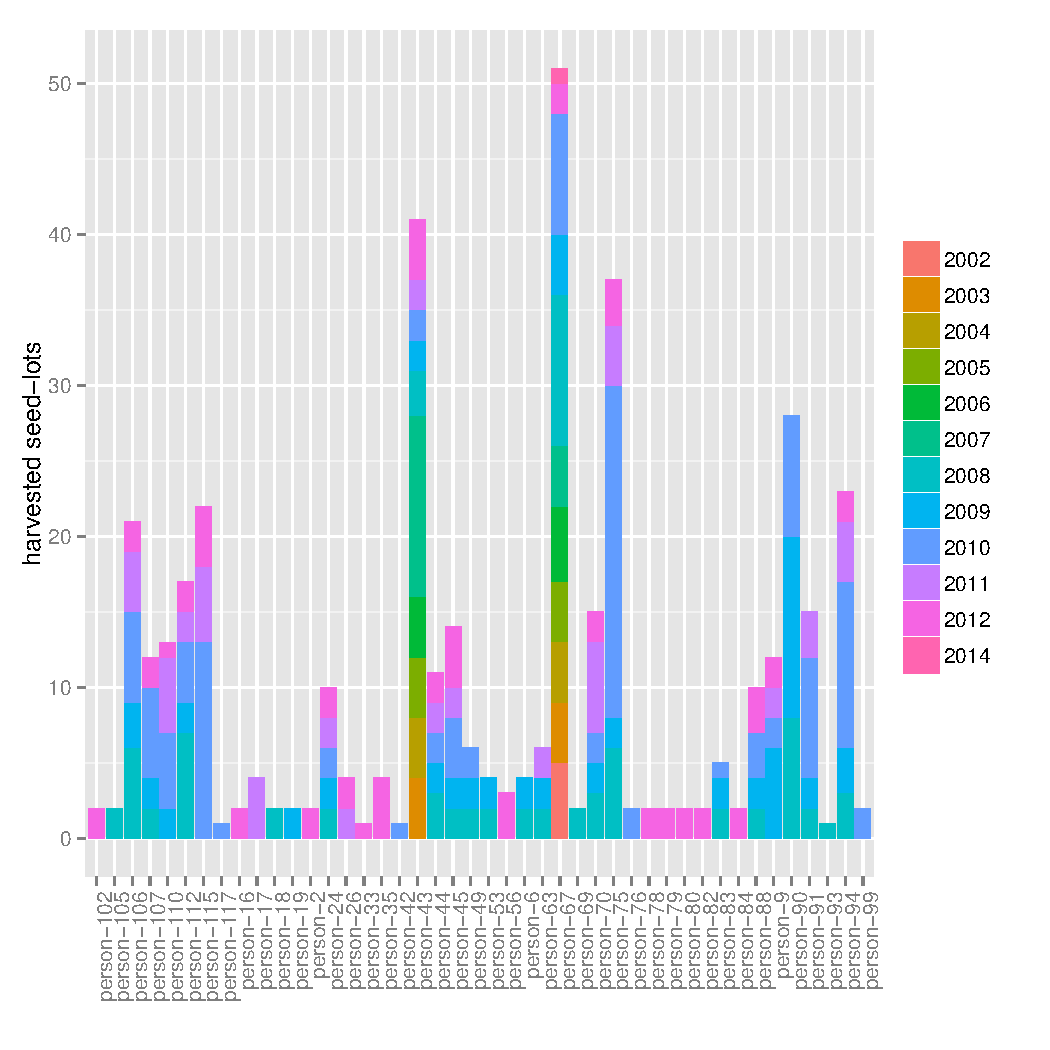
\includegraphics[width=.4\textwidth]{figures/shinemas2R_unnamed-chunk-31-1} 

}



\end{knitrout}
\\
\end{tabular}
\end{center}

\item Custom arguments

It is possible to tune the following arguments:

\begin{center}
\begin{table}[H]
\begin{tabular}{ p{.35\textwidth} p{.15\textwidth} p{.45\textwidth} }
\hline
argument & default value & description \\
\hline

\texttt{x.axis} & \texttt{NULL} & factor display on the x.axis of a plot: \texttt{"germplasm"}, \texttt{"year"} or \texttt{"person"} referring to the attributes of a seed-lots. If NULL, all the combinaison are done for \texttt{x.axis} and \texttt{in.col}. \\
\hline

\texttt{in.col} & \texttt{NULL} & display in color of a plot: \texttt{"germplasm"}, \texttt{"year"} or \texttt{"person"} referring to the attributes of a seed-lots. If \texttt{NULL}, \texttt{in.col} is not displayed. \\
\hline

\texttt{nb\_parameters\_per\_plot\_x.axis} & \texttt{NULL} & the number of parameters per plot on \texttt{x.axis} argument \\
\hline

\texttt{nb\_parameters\_per\_plot\_in.col} & \texttt{NULL} & the number of parameters per plot for \texttt{in.col} argument \\

\hline
\end{tabular}
\caption{Possible arguments to custom arguments regarding barplot.}
\label{custom.barplot}
\end{table}
\end{center}



For example, for a given \texttt{x.axis} and a given \texttt{in.col}:
\begin{knitrout}
\definecolor{shadecolor}{rgb}{0.969, 0.969, 0.969}\color{fgcolor}\begin{kframe}
\begin{alltt}
\hlstd{p_slh} \hlkwb{=} \hlkwd{get.ggplot}\hlstd{(}
        \hlstd{data_network,}
        \hlkwc{ggplot.type} \hlstd{=} \hlstr{"network-reproduction-harvested"}\hlstd{,}
        \hlkwc{ggplot.display} \hlstd{=} \hlstr{"barplot"}\hlstd{,}
        \hlkwc{x.axis} \hlstd{=} \hlstr{"person"}\hlstd{,}
        \hlkwc{in.col} \hlstd{=} \hlstr{"year"}
        \hlstd{)}
\end{alltt}
\end{kframe}
\end{knitrout}

It can be useful to separate the plot in several plots regarding \texttt{x.axis}:
\begin{knitrout}
\definecolor{shadecolor}{rgb}{0.969, 0.969, 0.969}\color{fgcolor}\begin{kframe}
\begin{alltt}
\hlstd{p1_slh} \hlkwb{=} \hlkwd{get.ggplot}\hlstd{(}
        \hlstd{data_network,}
        \hlkwc{ggplot.type} \hlstd{=} \hlstr{"network-reproduction-harvested"}\hlstd{,}
        \hlkwc{ggplot.display} \hlstd{=} \hlstr{"barplot"}\hlstd{,}
        \hlkwc{x.axis} \hlstd{=} \hlstr{"person"}\hlstd{,}
        \hlkwc{in.col} \hlstd{=} \hlstr{"year"}\hlstd{,}
        \hlkwc{nb_parameters_per_plot_x.axis} \hlstd{=} \hlnum{10}
        \hlstd{)}

\hlstd{p11_slh} \hlkwb{=} \hlstd{p1_slh}\hlopt{$}\hlstd{`network-reproduction-harvested`}\hlopt{$}\hlstd{barplot}\hlopt{$}\hlstd{`person-year`}\hlopt{$}\hlstd{`x.axis-1|in.col-1`}
\hlstd{p12_slh} \hlkwb{=} \hlstd{p1_slh}\hlopt{$}\hlstd{`network-reproduction-harvested`}\hlopt{$}\hlstd{barplot}\hlopt{$}\hlstd{`person-year`}\hlopt{$}\hlstd{`x.axis-2|in.col-1`}
\hlstd{p13_slh} \hlkwb{=} \hlstd{p1_slh}\hlopt{$}\hlstd{`network-reproduction-harvested`}\hlopt{$}\hlstd{barplot}\hlopt{$}\hlstd{`person-year`}\hlopt{$}\hlstd{`x.axis-3|in.col-1`}
\hlstd{p14_slh} \hlkwb{=} \hlstd{p1_slh}\hlopt{$}\hlstd{`network-reproduction-harvested`}\hlopt{$}\hlstd{barplot}\hlopt{$}\hlstd{`person-year`}\hlopt{$}\hlstd{`x.axis-4|in.col-1`}
\hlstd{p15_slh} \hlkwb{=} \hlstd{p1_slh}\hlopt{$}\hlstd{`network-reproduction-harvested`}\hlopt{$}\hlstd{barplot}\hlopt{$}\hlstd{`person-year`}\hlopt{$}\hlstd{`x.axis-5|in.col-1`}
\end{alltt}
\end{kframe}
\end{knitrout}


Note that you can easily change settings of the plot as it is a ggplot object, for example
\begin{knitrout}
\definecolor{shadecolor}{rgb}{0.969, 0.969, 0.969}\color{fgcolor}\begin{kframe}
\begin{alltt}
\hlstd{p15_slh_bw} \hlkwb{=} \hlstd{p15_slh} \hlopt{+} \hlkwd{theme_bw}\hlstd{()}
\end{alltt}
\end{kframe}
\end{knitrout}


\begin{center}
\begin{tabular}{cc}
\texttt{p11\_slh} & \texttt{p12\_slh} \\
\begin{knitrout}
\definecolor{shadecolor}{rgb}{0.969, 0.969, 0.969}\color{fgcolor}

{\centering 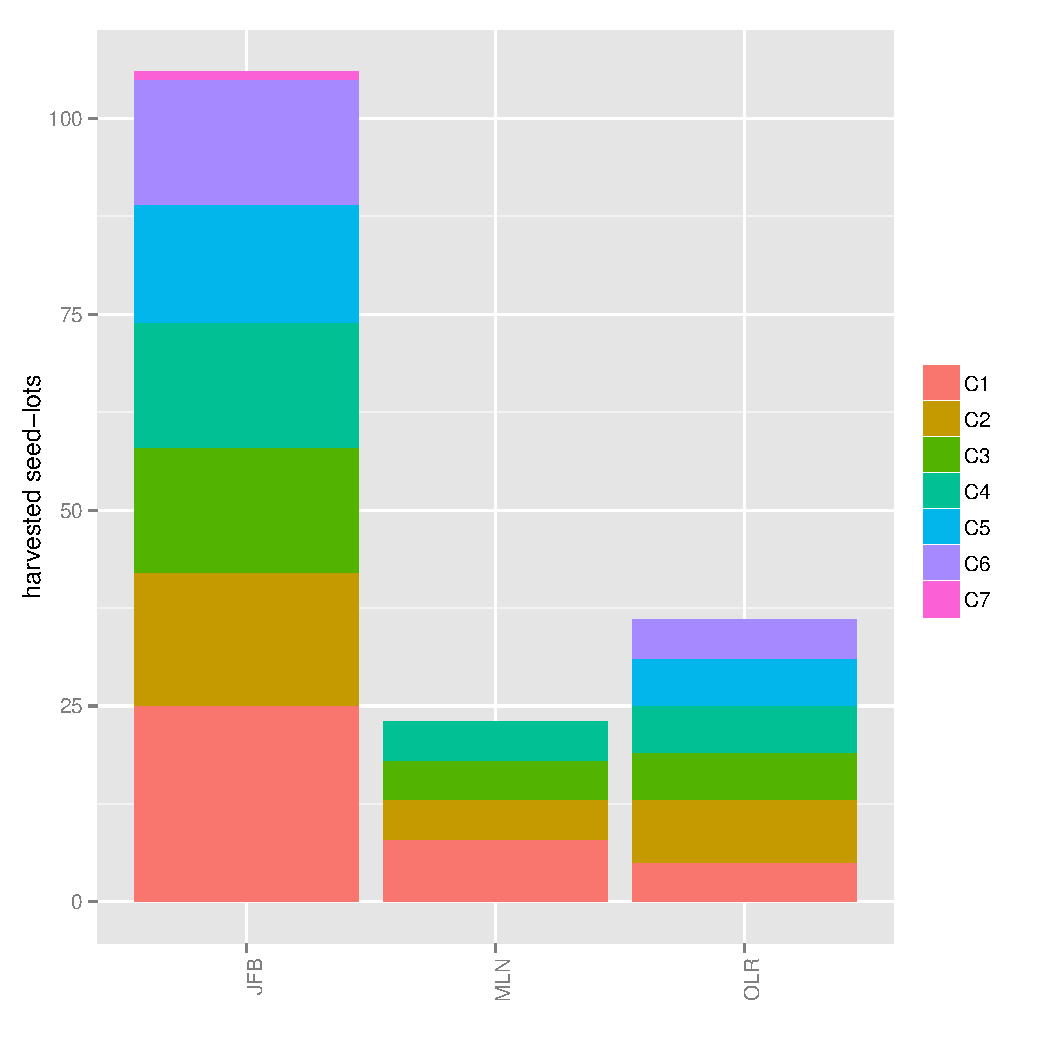
\includegraphics[width=.4\textwidth]{figures/shinemas2R_unnamed-chunk-35-1} 

}



\end{knitrout}
&
\begin{knitrout}
\definecolor{shadecolor}{rgb}{0.969, 0.969, 0.969}\color{fgcolor}

{\centering 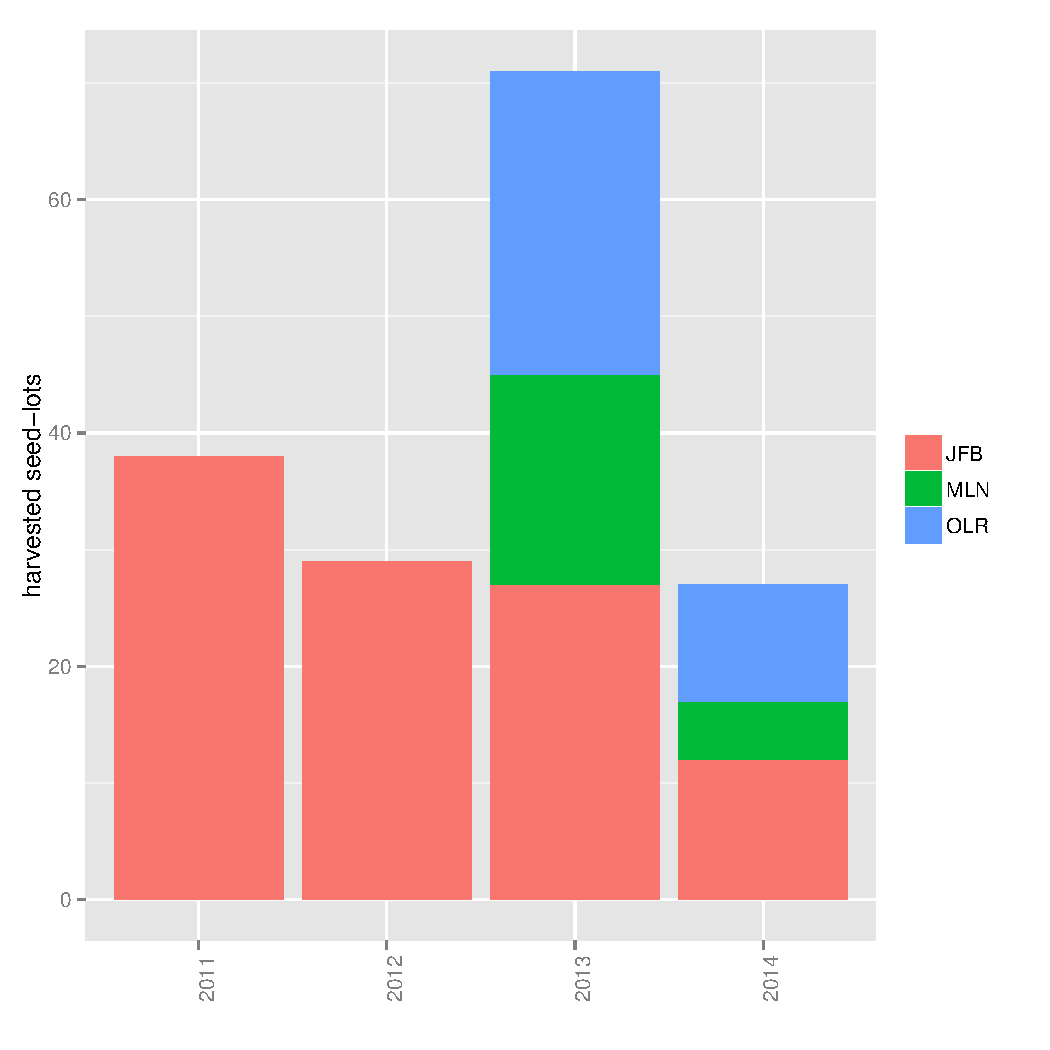
\includegraphics[width=.4\textwidth]{figures/shinemas2R_unnamed-chunk-36-1} 

}



\end{knitrout}
\\
\texttt{p13\_slh} & \texttt{p14\_slh} \\
\begin{knitrout}
\definecolor{shadecolor}{rgb}{0.969, 0.969, 0.969}\color{fgcolor}

{\centering 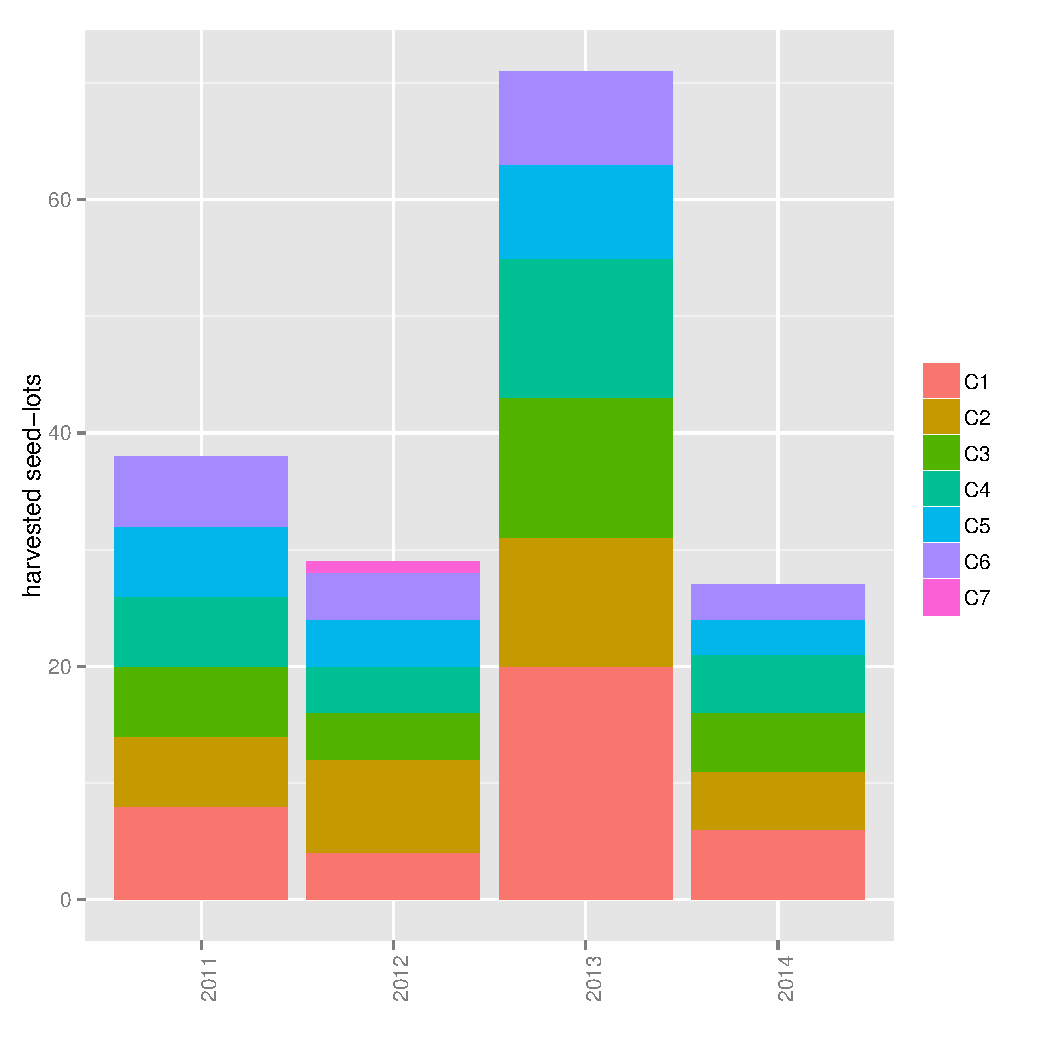
\includegraphics[width=.4\textwidth]{figures/shinemas2R_unnamed-chunk-37-1} 

}



\end{knitrout}
&
\begin{knitrout}
\definecolor{shadecolor}{rgb}{0.969, 0.969, 0.969}\color{fgcolor}

{\centering 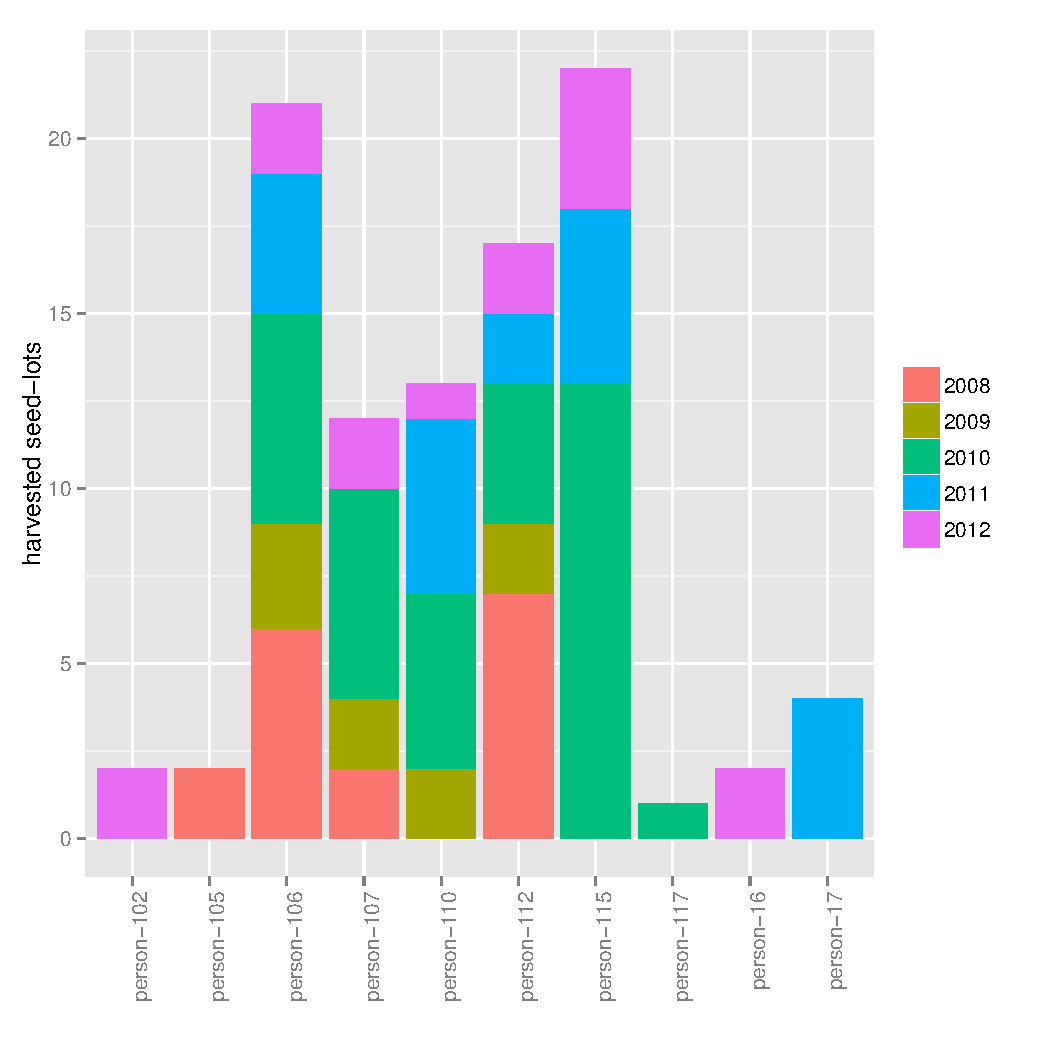
\includegraphics[width=.4\textwidth]{figures/shinemas2R_unnamed-chunk-38-1} 

}



\end{knitrout}
\\
\texttt{p15\_slh} & \texttt{p15\_slh\_bw}  \\
\begin{knitrout}
\definecolor{shadecolor}{rgb}{0.969, 0.969, 0.969}\color{fgcolor}

{\centering 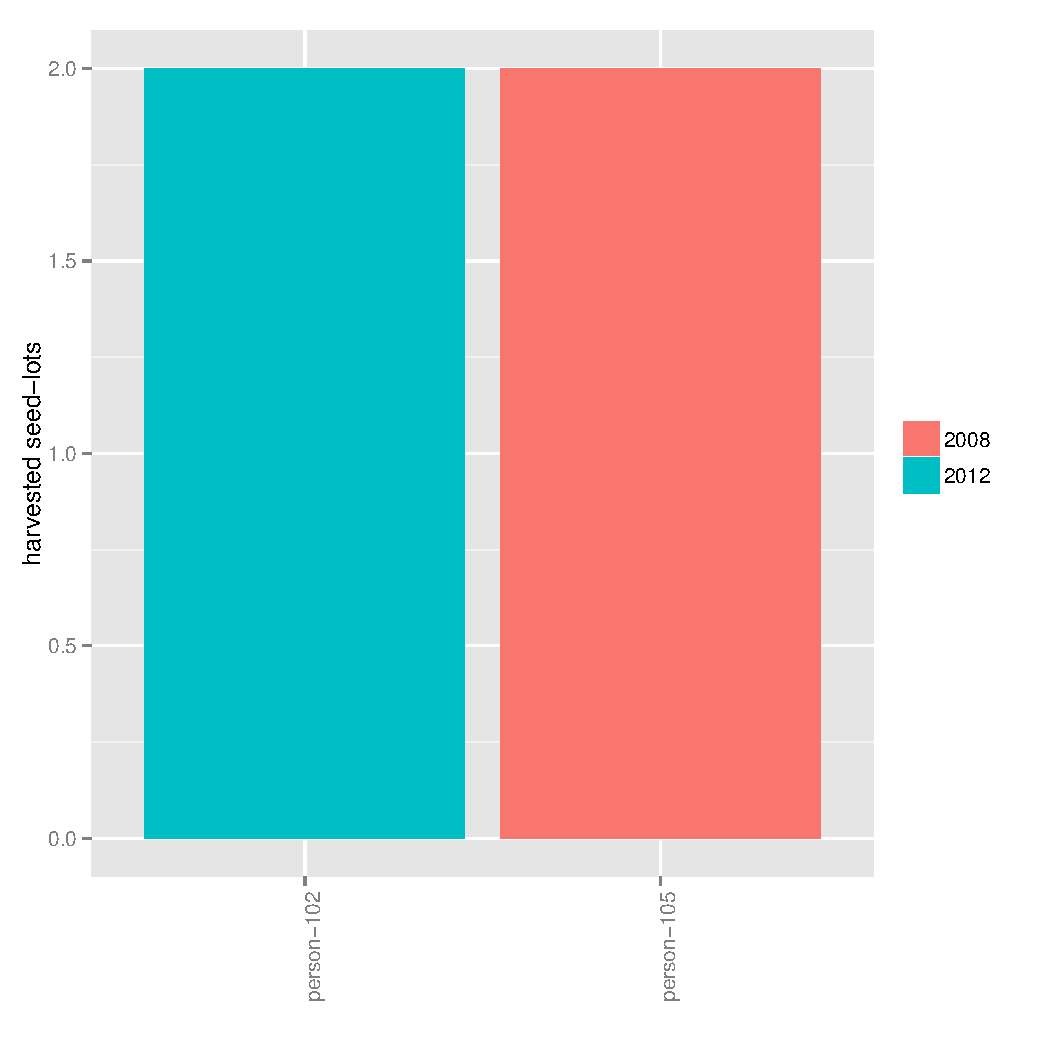
\includegraphics[width=.4\textwidth]{figures/shinemas2R_unnamed-chunk-39-1} 

}



\end{knitrout}
&
\begin{knitrout}
\definecolor{shadecolor}{rgb}{0.969, 0.969, 0.969}\color{fgcolor}

{\centering 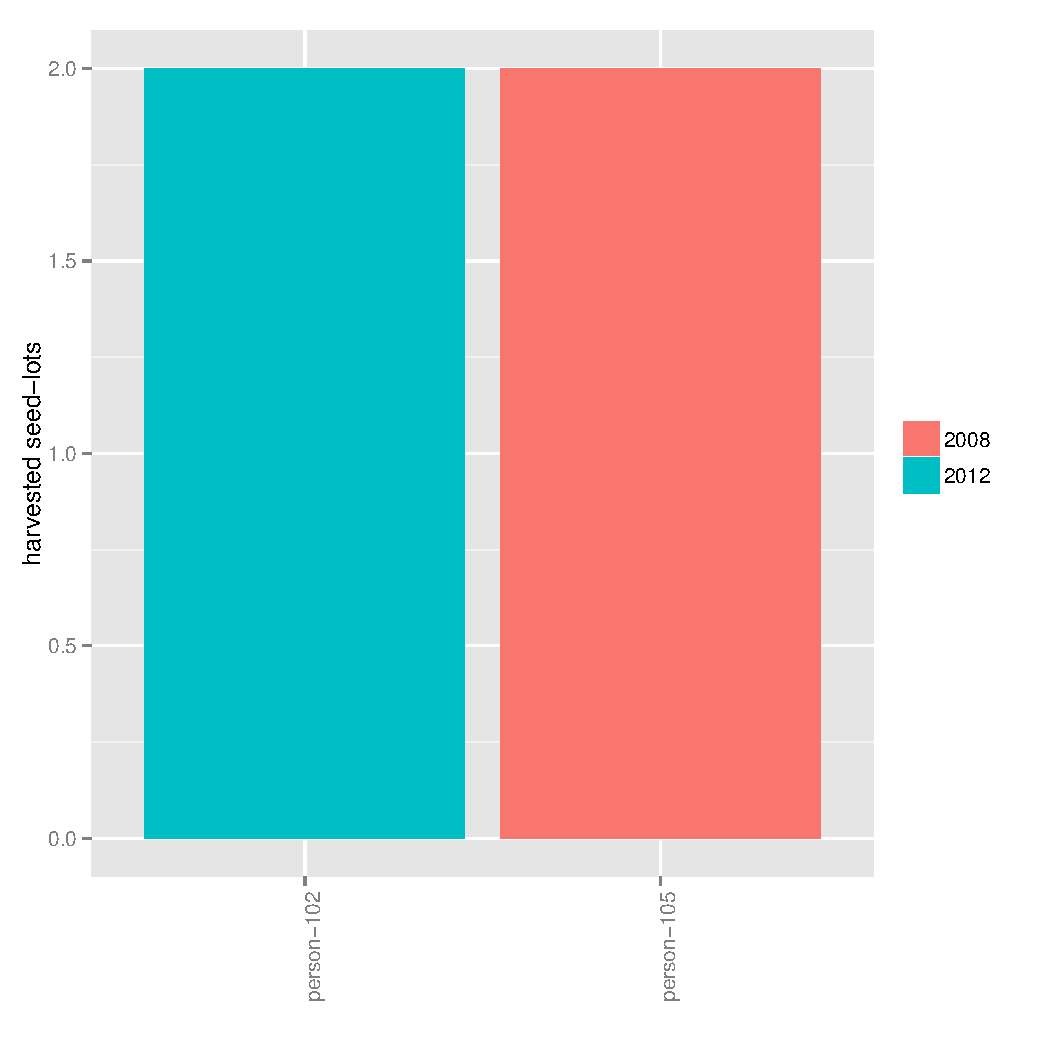
\includegraphics[width=.4\textwidth]{figures/shinemas2R_unnamed-chunk-40-1} 

}



\end{knitrout}
\\
\end{tabular}
\end{center}



Or for \texttt{in.col}:
\begin{knitrout}
\definecolor{shadecolor}{rgb}{0.969, 0.969, 0.969}\color{fgcolor}\begin{kframe}
\begin{alltt}
\hlstd{p2_slh} \hlkwb{=} \hlkwd{get.ggplot}\hlstd{(}
        \hlstd{data_network,}
        \hlkwc{ggplot.type} \hlstd{=} \hlstr{"network-reproduction-harvested"}\hlstd{,}
        \hlkwc{ggplot.display} \hlstd{=} \hlstr{"barplot"}\hlstd{,}
        \hlkwc{x.axis} \hlstd{=} \hlstr{"person"}\hlstd{,}
        \hlkwc{in.col} \hlstd{=} \hlstr{"year"}\hlstd{,}
        \hlkwc{nb_parameters_per_plot_in.col} \hlstd{=} \hlnum{3}
        \hlstd{)}

\hlstd{p21_slh} \hlkwb{=} \hlstd{p2_slh}\hlopt{$}\hlstd{`network-reproduction-harvested`}\hlopt{$}\hlstd{barplot}\hlopt{$}\hlstd{`person-year`}\hlopt{$}\hlstd{`x.axis-1|in.col-1`}
\hlstd{p22_slh} \hlkwb{=} \hlstd{p2_slh}\hlopt{$}\hlstd{`network-reproduction-harvested`}\hlopt{$}\hlstd{barplot}\hlopt{$}\hlstd{`person-year`}\hlopt{$}\hlstd{`x.axis-1|in.col-2`}
\hlstd{p23_slh} \hlkwb{=} \hlstd{p2_slh}\hlopt{$}\hlstd{`network-reproduction-harvested`}\hlopt{$}\hlstd{barplot}\hlopt{$}\hlstd{`person-year`}\hlopt{$}\hlstd{`x.axis-1|in.col-3`}
\end{alltt}
\end{kframe}
\end{knitrout}

\begin{center}
\begin{tabular}{cc}
\texttt{p21\_slh} & \texttt{p22\_slh} \\
\begin{knitrout}
\definecolor{shadecolor}{rgb}{0.969, 0.969, 0.969}\color{fgcolor}

{\centering 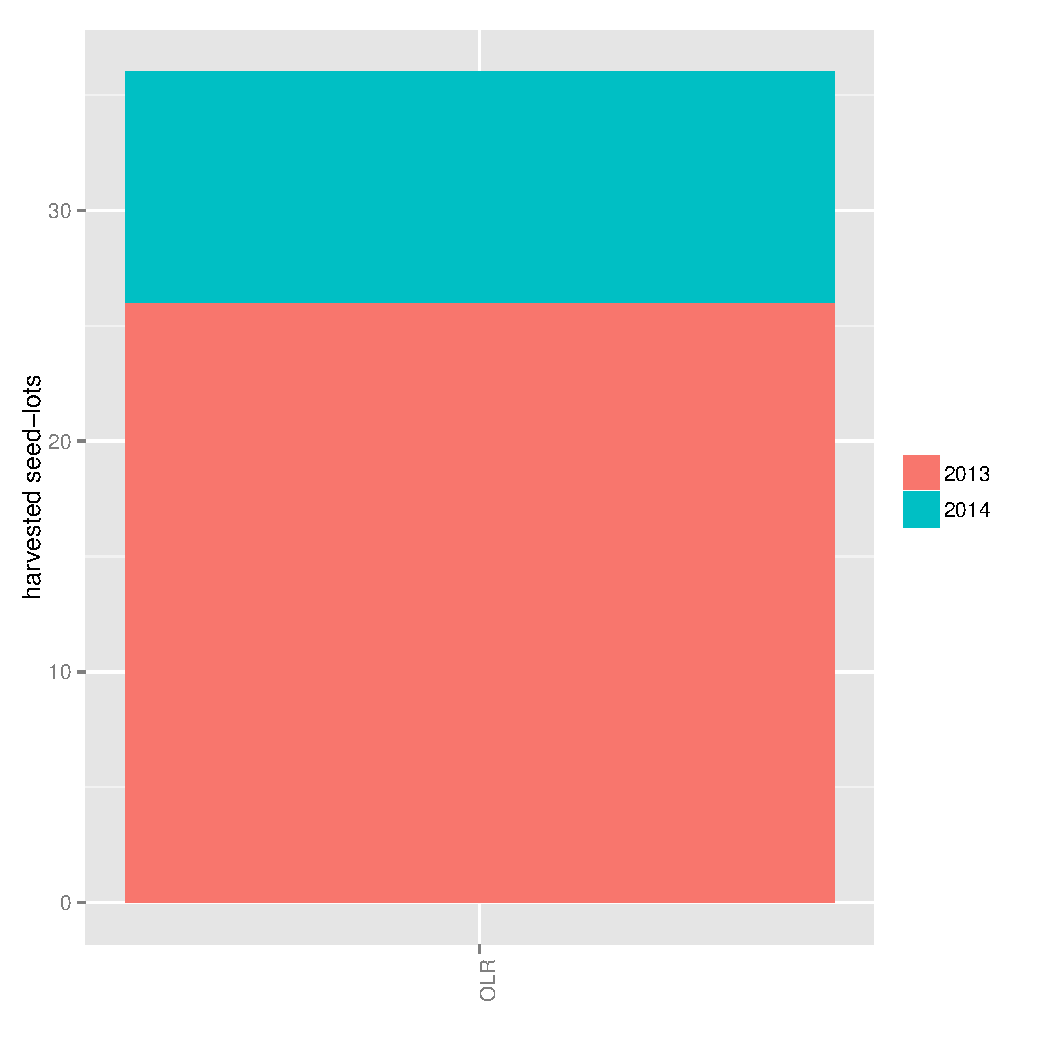
\includegraphics[width=.4\textwidth]{figures/shinemas2R_unnamed-chunk-42-1} 

}



\end{knitrout}
&
\begin{knitrout}
\definecolor{shadecolor}{rgb}{0.969, 0.969, 0.969}\color{fgcolor}

{\centering 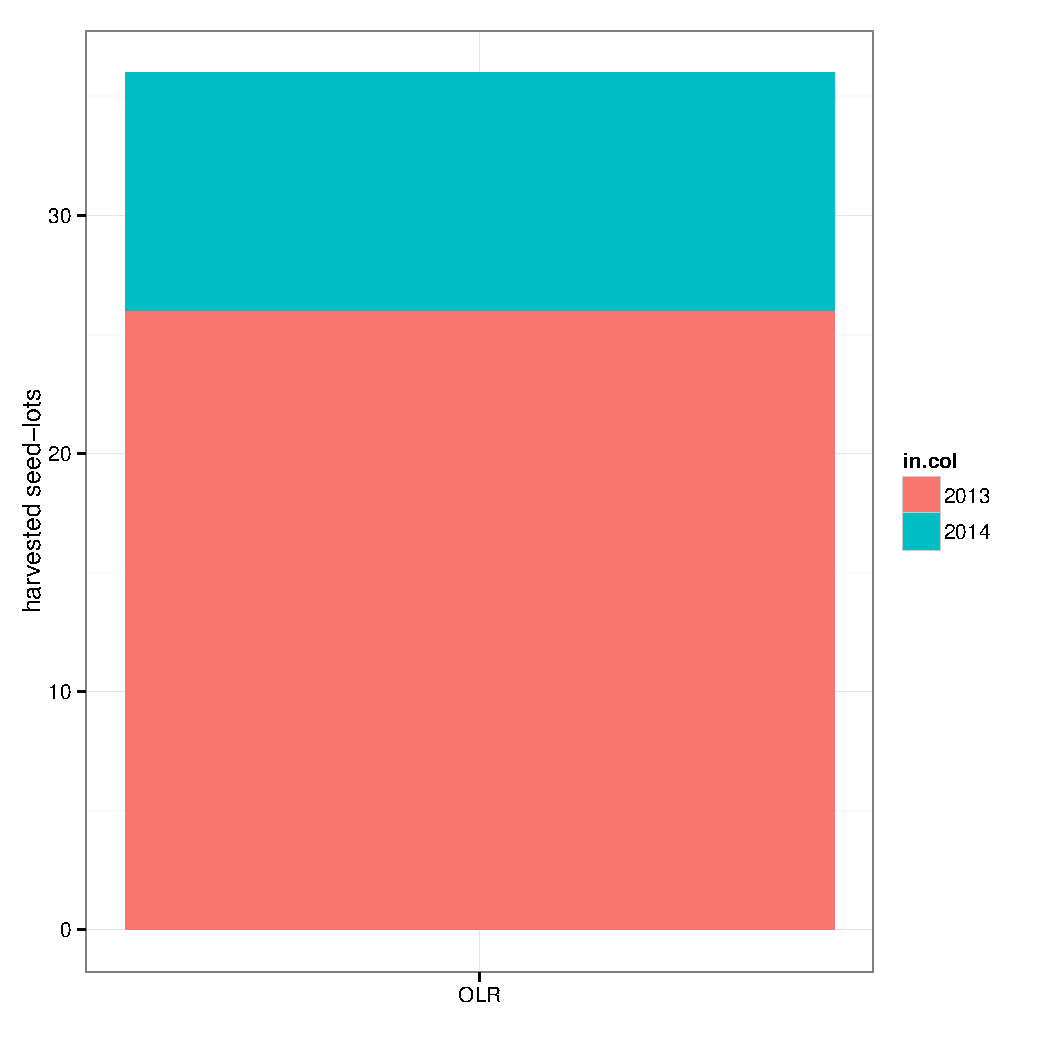
\includegraphics[width=.4\textwidth]{figures/shinemas2R_unnamed-chunk-43-1} 

}



\end{knitrout}
\\
\texttt{p23\_slh} & \\
\begin{knitrout}
\definecolor{shadecolor}{rgb}{0.969, 0.969, 0.969}\color{fgcolor}

{\centering 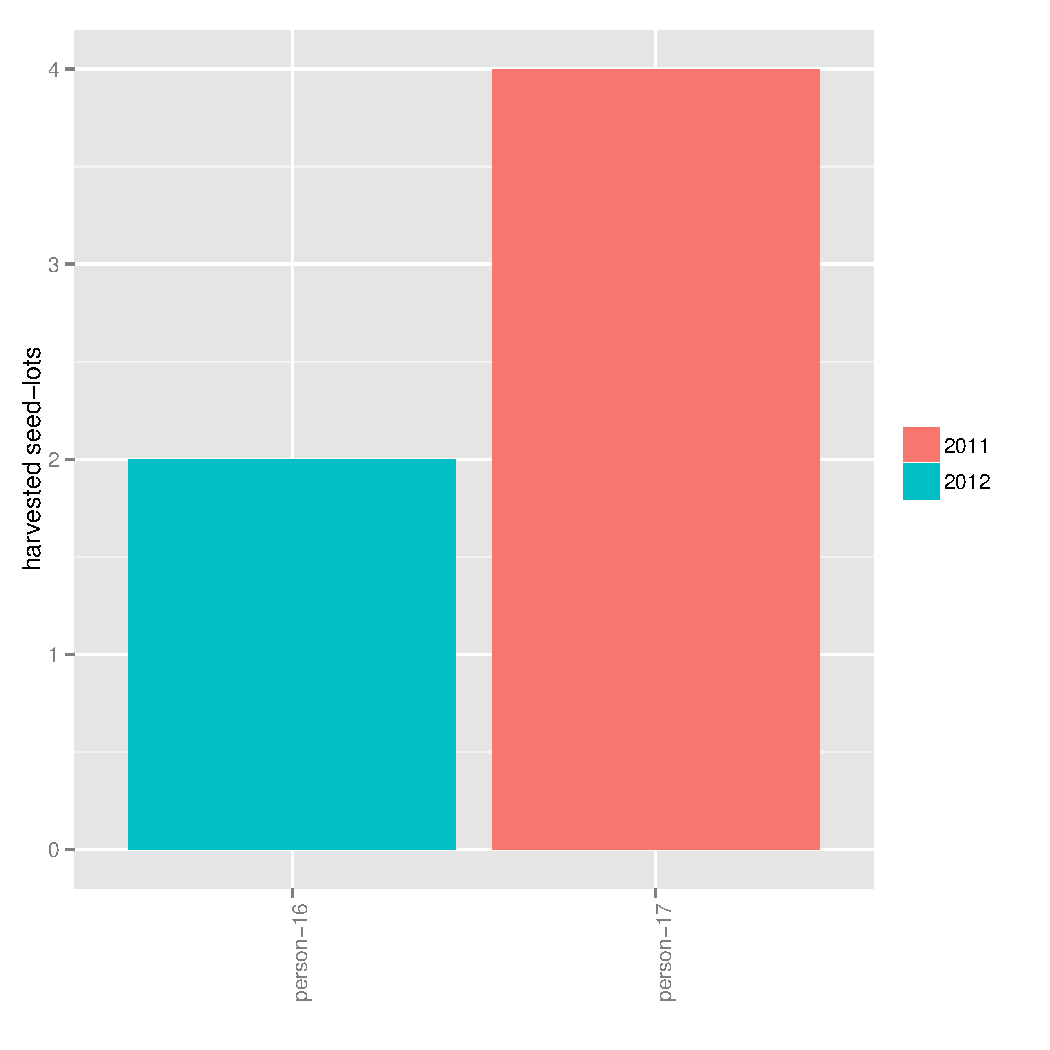
\includegraphics[width=.4\textwidth]{figures/shinemas2R_unnamed-chunk-44-1} 

}



\end{knitrout}
&
\\
\end{tabular}
\end{center}


Or for both, for each subset of \texttt{x.axis}, you have the set of \texttt{in.col}.

\end{itemize}


\paragraph{\texttt{ggplot.display = map}}

There are as many maps as years and a map with all the years mixed.
The scale represent the number of seed-lots harvected.

\begin{itemize}

\item Default arguments

\begin{knitrout}
\definecolor{shadecolor}{rgb}{0.969, 0.969, 0.969}\color{fgcolor}\begin{kframe}
\begin{alltt}
\hlstd{m_slh} \hlkwb{=} \hlstd{default_network_ggplot}\hlopt{$}\hlstd{`network-reproduction-harvested`}\hlopt{$}\hlstd{map}
\hlkwd{names}\hlstd{(m_slh)}
\end{alltt}
\begin{verbatim}
## [1] "map-[2002]"                                          
## [2] "map-[2006]"                                          
## [3] "map-[2008]"                                          
## [4] "map-[2009]"                                          
## [5] "map-[2010]"                                          
## [6] "map-[2011]"                                          
## [7] "map-[2012]"                                          
## [8] "map-[2014]"                                          
## [9] "map-[2002, 2006, 2008, 2009, 2010, 2011, 2012, 2014]"
\end{verbatim}
\begin{alltt}
\hlstd{m4_slh} \hlkwb{=} \hlstd{m_slh}\hlopt{$}\hlstd{`map-[2011]`}
\hlstd{m9_slh} \hlkwb{=} \hlstd{m_slh}\hlopt{$}\hlstd{`map-[2002, 2006, 2008, 2009, 2010, 2011, 2012, 2014]`}
\end{alltt}
\end{kframe}
\end{knitrout}

\begin{center}
\begin{tabular}{cc}
\texttt{m4\_slh} & \texttt{m9\_slh} \\
\begin{knitrout}
\definecolor{shadecolor}{rgb}{0.969, 0.969, 0.969}\color{fgcolor}

{\centering 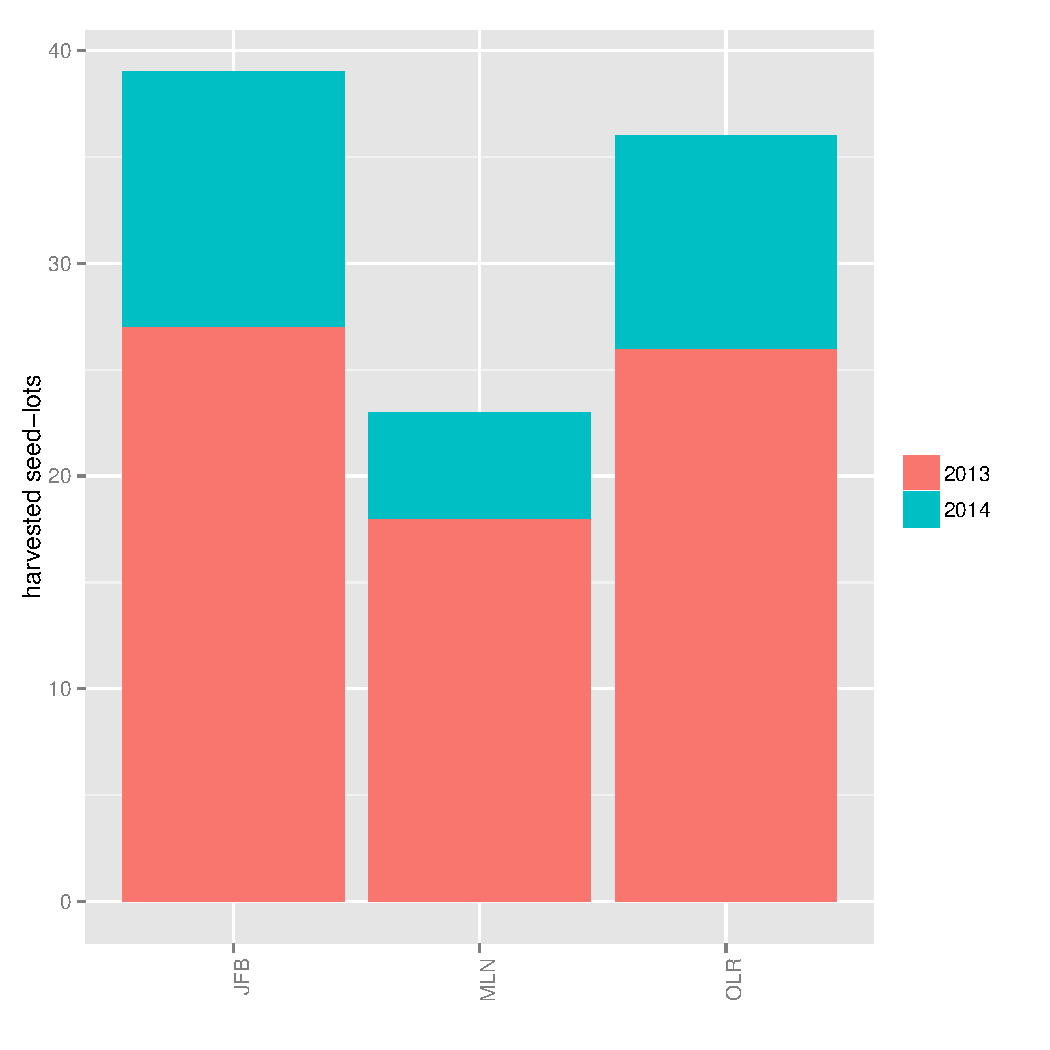
\includegraphics[width=.4\textwidth]{figures/shinemas2R_unnamed-chunk-46-1} 

}



\end{knitrout}
&
\begin{knitrout}
\definecolor{shadecolor}{rgb}{0.969, 0.969, 0.969}\color{fgcolor}

{\centering 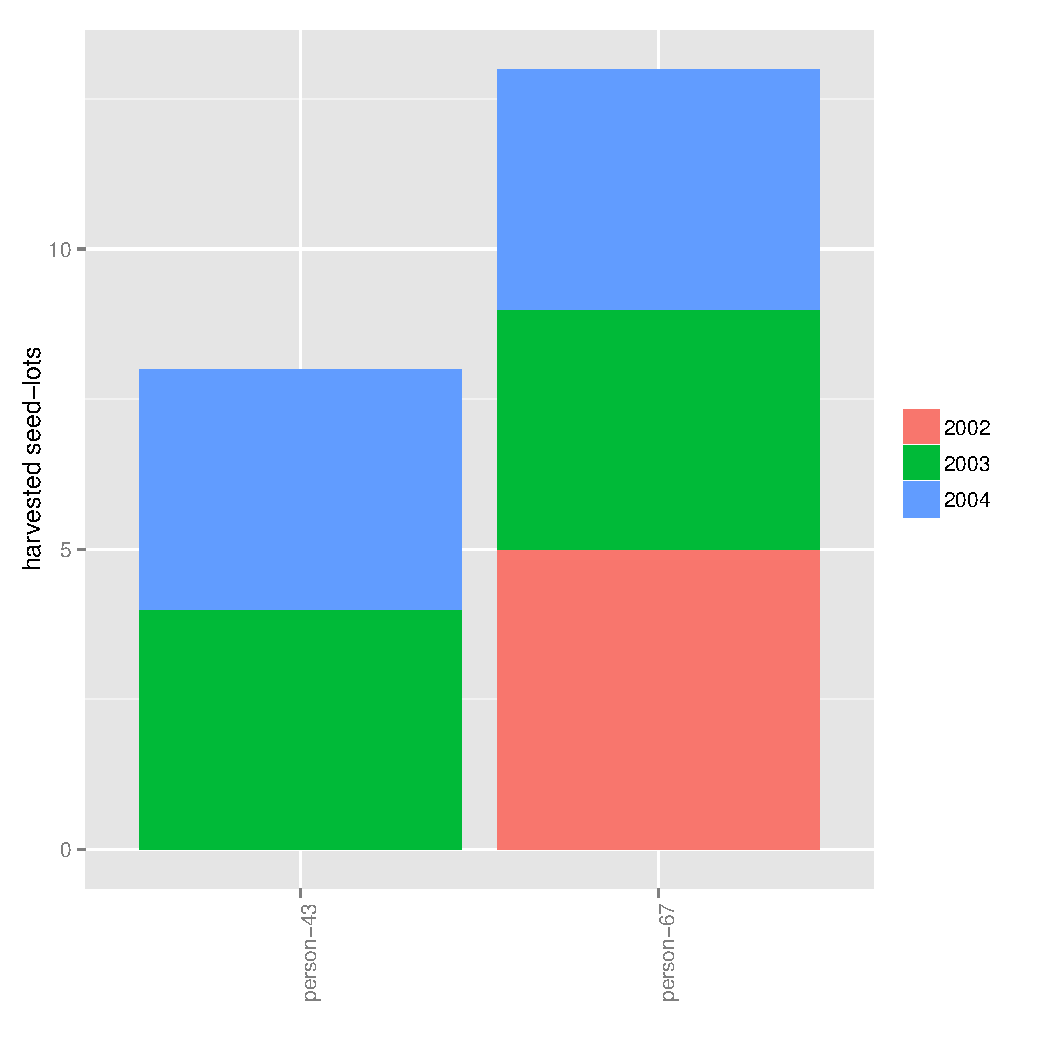
\includegraphics[width=.4\textwidth]{figures/shinemas2R_unnamed-chunk-47-1} 

}



\end{knitrout}
\\
\end{tabular}
\end{center}


\item Custom arguments

It is possible to tune the following arguments (Table \ref{custom.map}):

\begin{center}
\begin{table}[H]
\begin{tabular}{ p{.2\textwidth} p{.15\textwidth} p{.5\textwidth} }
\hline
argument & default value & description \\
\hline

\texttt{hide.labels.parts} & \texttt{NULL} & can be NULL or "all" as only person can be display. \texttt{NULL} by default \\
\hline

\texttt{labels.size} & \texttt{3} & size of the labels \\
\hline

\texttt{location.map} & \texttt{"france"} & location of the map see \texttt{?map} for more details \\
\hline

\texttt{pie.size} & \texttt{.5} & size of the pie when using pies \\

\hline
\end{tabular}
\caption{Possible arguments to custom arguments regarding maps.}
\label{custom.map}
\end{table}
\end{center}

For example,

\begin{knitrout}
\definecolor{shadecolor}{rgb}{0.969, 0.969, 0.969}\color{fgcolor}\begin{kframe}
\begin{alltt}
\hlstd{p_slh} \hlkwb{=} \hlkwd{get.ggplot}\hlstd{(}
        \hlstd{data_network,}
        \hlkwc{ggplot.type} \hlstd{=} \hlstr{"network-reproduction-harvested"}\hlstd{,}
        \hlkwc{ggplot.display} \hlstd{=} \hlstr{"map"}\hlstd{,}
        \hlkwc{hide.labels.parts} \hlstd{=} \hlkwa{NULL}
        \hlstd{)}

\hlstd{p_slh}\hlopt{$}\hlstd{`network-reproduction-harvested`}\hlopt{$}\hlstd{map}\hlopt{$}\hlstd{`map-[2011]`}
\end{alltt}
\end{kframe}

{\centering 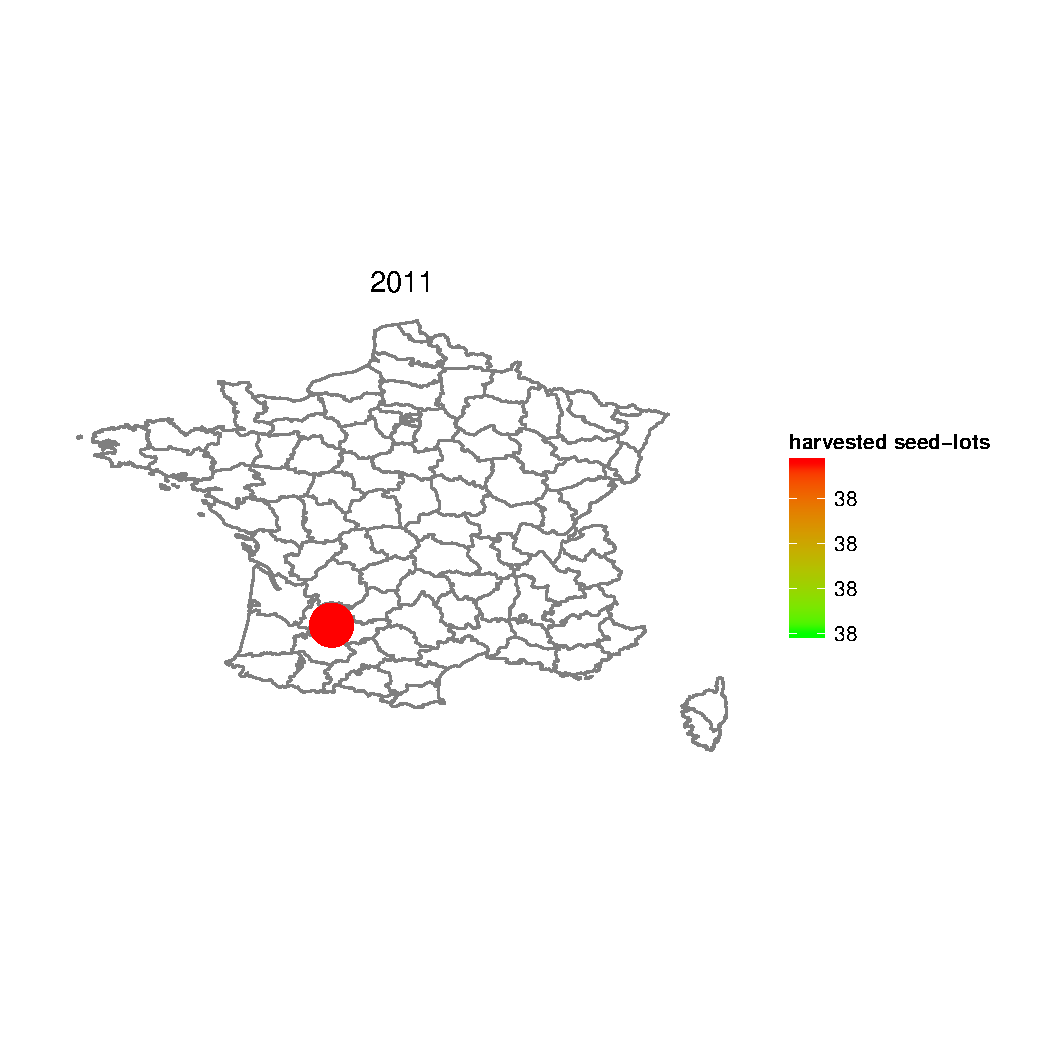
\includegraphics[width=.6\textwidth]{figures/shinemas2R_unnamed-chunk-48-1} 

}



\end{knitrout}

\end{itemize}

\subsubsection{\texttt{ggplot.type = "network-diffusion-relation"}}

\texttt{ggplot.type = "network-diffusion-relation"} corresponds to diffusion of seed-lots on a map.
Note that \texttt{ggplot.display} is useless here.

There are as many maps as years and a map with all the years mixed.
The size of the arrows is proprotionnal to the number of diffusions (\texttt{nb\_diffusions}).

\begin{itemize}

\item Default arguments

\begin{knitrout}
\definecolor{shadecolor}{rgb}{0.969, 0.969, 0.969}\color{fgcolor}\begin{kframe}
\begin{alltt}
\hlstd{m_dr} \hlkwb{=} \hlstd{default_network_ggplot}\hlopt{$}\hlstd{`network-diffusion-relation`}\hlopt{$}\hlstd{map}
\hlkwd{names}\hlstd{(m_dr)}
\end{alltt}
\begin{verbatim}
## [1] "map-[2002]"                              
## [2] "map-[2007]"                              
## [3] "map-[2008]"                              
## [4] "map-[2009]"                              
## [5] "map-[2010]"                              
## [6] "map-[2011]"                              
## [7] "map-[2002, 2007, 2008, 2009, 2010, 2011]"
\end{verbatim}
\begin{alltt}
\hlstd{m4_dr} \hlkwb{=} \hlstd{m_dr}\hlopt{$}\hlstd{`map-[2009]`}
\hlstd{m7_dr} \hlkwb{=} \hlstd{m_dr}\hlopt{$}\hlstd{`map-[2002, 2007, 2008, 2009, 2010, 2011]`}
\end{alltt}
\end{kframe}
\end{knitrout}

\begin{center}
\begin{tabular}{cc}
\texttt{m4\_dr} & \texttt{m7\_dr} \\
\begin{knitrout}
\definecolor{shadecolor}{rgb}{0.969, 0.969, 0.969}\color{fgcolor}

{\centering 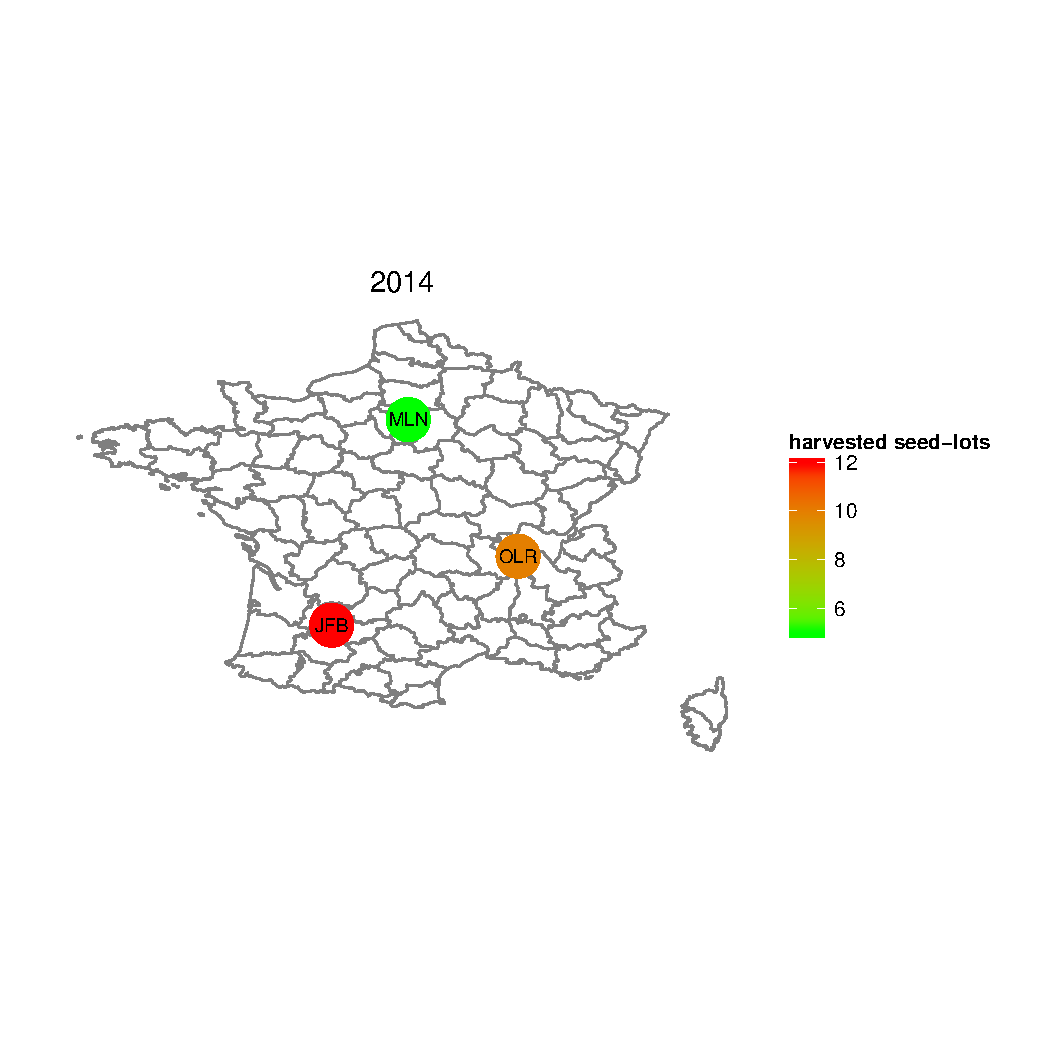
\includegraphics[width=.4\textwidth]{figures/shinemas2R_unnamed-chunk-50-1} 

}



\end{knitrout}
&
\begin{knitrout}
\definecolor{shadecolor}{rgb}{0.969, 0.969, 0.969}\color{fgcolor}

{\centering 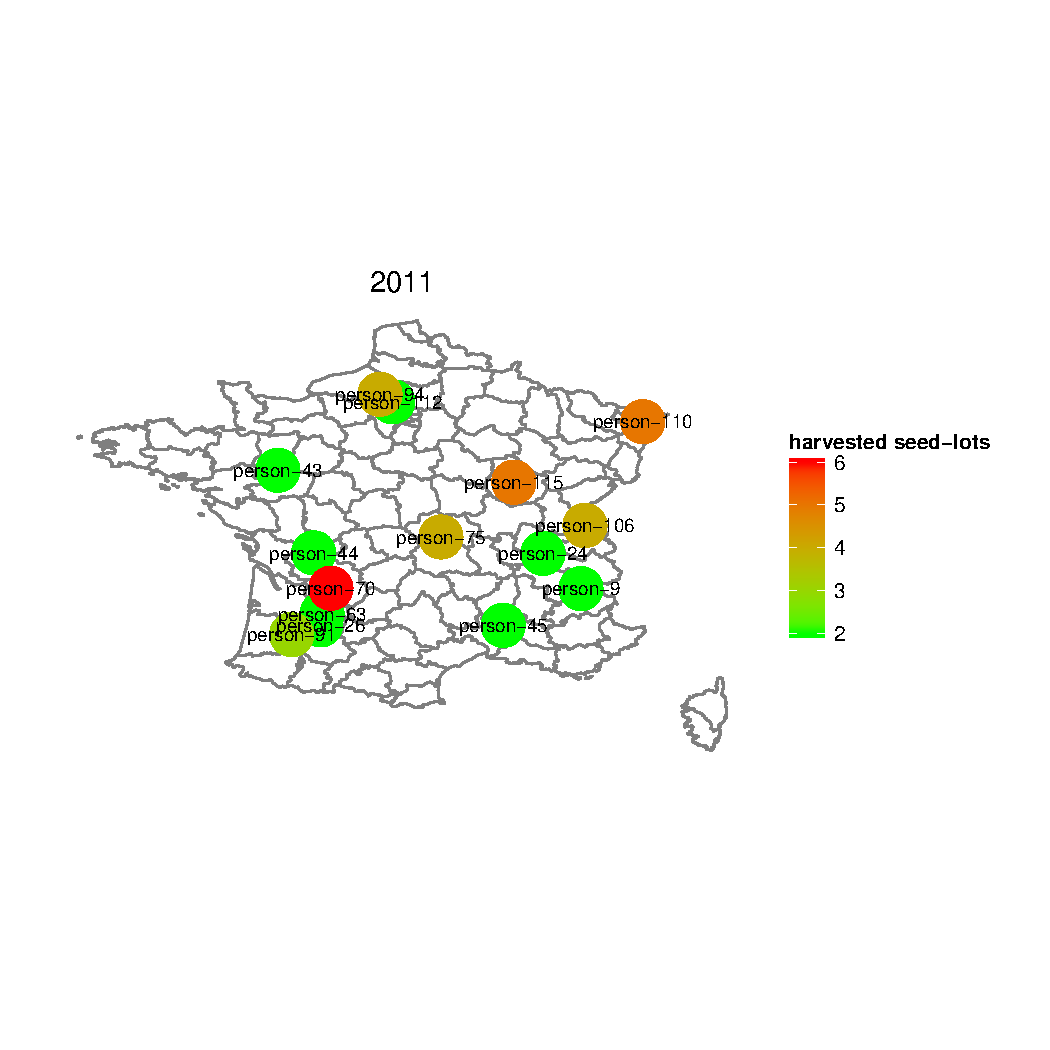
\includegraphics[width=.4\textwidth]{figures/shinemas2R_unnamed-chunk-51-1} 

}



\end{knitrout}
\\
\end{tabular}
\end{center}


\item Custom arguments

Arguments can be customed related to maps. See Table \ref{custom.map}.

\end{itemize}


\subsubsection{\texttt{ggplot.type = "network-reproduction-crossed"}}

Information on the crosses, their parents (mother and father) and grandparents (grandmother and grandfather).
It may be useful to know information on grandparents, especially location, if the cross have been done on another location.

Note that in this example, it represents all the cross where \texttt{Rouge-du-Roc} is involved as \texttt{"father"} or \texttt{"son"} in relation.
This is because in \texttt{get.data}, the following arguments were set: \texttt{germplasm.in = Rouge-du-Roc} and \texttt{filter.on = "father-son"}.


\begin{itemize}

\item Default arguments

\begin{knitrout}
\definecolor{shadecolor}{rgb}{0.969, 0.969, 0.969}\color{fgcolor}\begin{kframe}
\begin{alltt}
\hlstd{cb} \hlkwb{=} \hlstd{default_network_ggplot}\hlopt{$}\hlstd{`network-reproduction-crossed`}\hlopt{$}\hlstd{barplot}
\hlkwd{names}\hlstd{(cb)}
\end{alltt}
\begin{verbatim}
## [1] "cross"       "father"      "grandfather" "mother"     
## [5] "grandmother"
\end{verbatim}
\begin{alltt}
\hlstd{cm} \hlkwb{=} \hlstd{default_network_ggplot}\hlopt{$}\hlstd{`network-reproduction-crossed`}\hlopt{$}\hlstd{map}
\hlkwd{names}\hlstd{(cm)}
\end{alltt}
\begin{verbatim}
## [1] "cross"       "father"      "grandfather" "mother"     
## [5] "grandmother"
\end{verbatim}
\end{kframe}
\end{knitrout}

For example:

\begin{knitrout}
\definecolor{shadecolor}{rgb}{0.969, 0.969, 0.969}\color{fgcolor}\begin{kframe}
\begin{alltt}
\hlstd{cb}\hlopt{$}\hlstd{cross}\hlopt{$}\hlstd{barplot}\hlopt{$}\hlstd{`year-germplasm`}\hlopt{$}\hlstd{`x.axis-1|in.col-1`}
\end{alltt}
\end{kframe}

{\centering 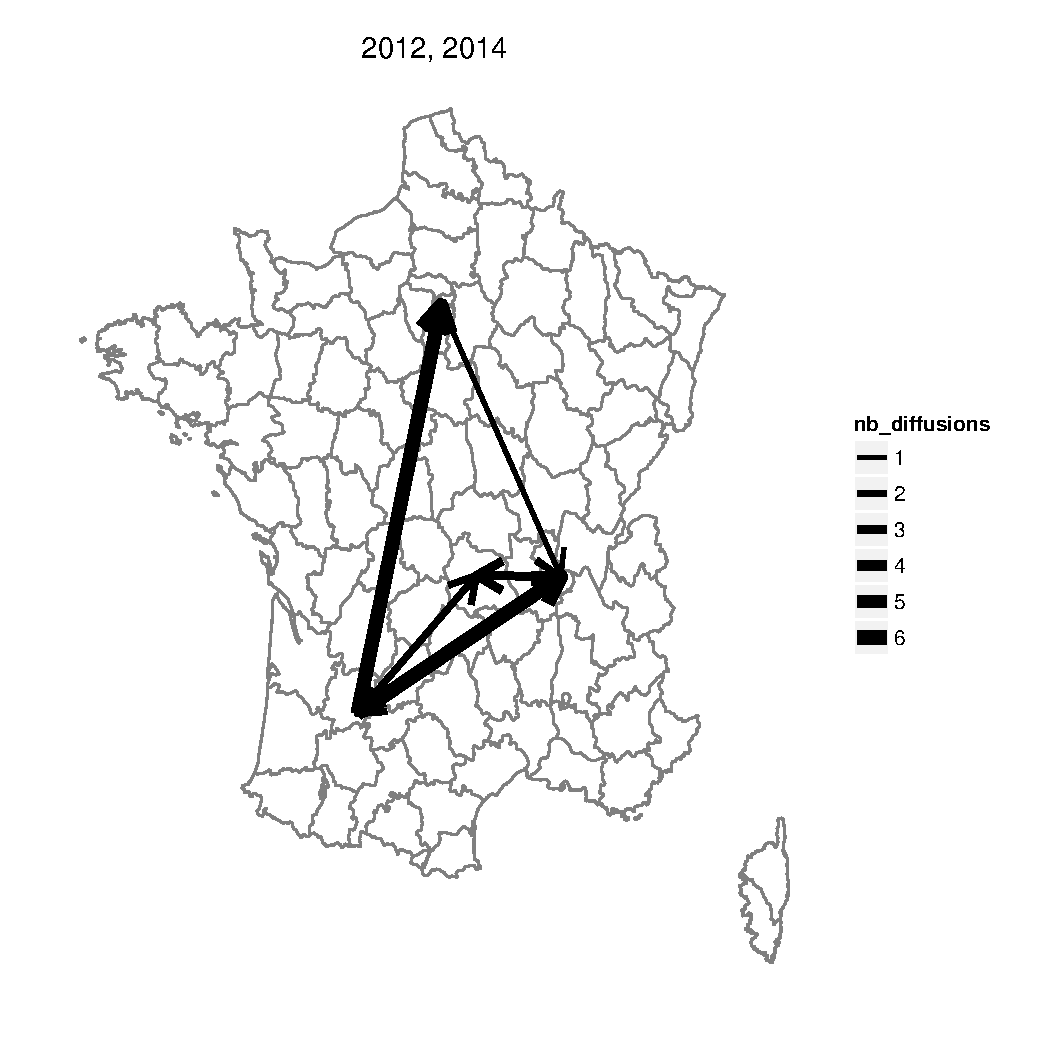
\includegraphics[width=.6\textwidth]{figures/shinemas2R_unnamed-chunk-53-1} 

}



\end{knitrout}

\begin{knitrout}
\definecolor{shadecolor}{rgb}{0.969, 0.969, 0.969}\color{fgcolor}\begin{kframe}
\begin{alltt}
\hlstd{cm}\hlopt{$}\hlstd{cross}\hlopt{$}\hlstd{map}\hlopt{$}\hlstd{`map-[2002, 2008, 2009]`}
\end{alltt}
\end{kframe}

{\centering 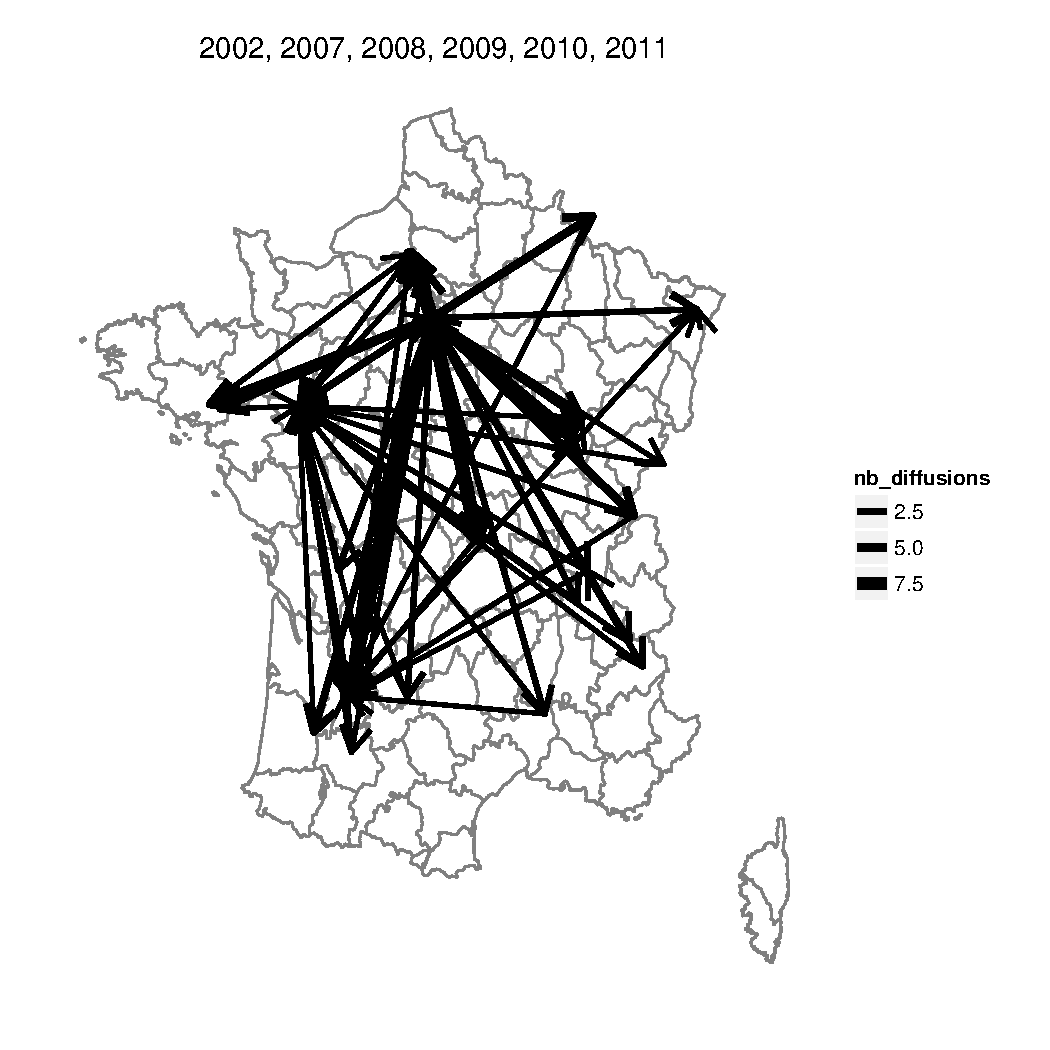
\includegraphics[width=.6\textwidth]{figures/shinemas2R_unnamed-chunk-54-1} 

}



\end{knitrout}

\item Custom arguments

Arguments can be customed related to barplots (Table \ref{custom.barplot}) or maps (Table \ref{custom.map}).

\end{itemize}

\subsubsection{Others \texttt{ggplot.type}}

For the others \texttt{ggplot.type}, as it is exactly the same types of plots than for
\texttt{ggplot.type = "network-reproduction-harvested"}, no examples are displayed in this vignette.

The following table describe the different \texttt{ggplot.type}:

\begin{center}
\begin{tabular}{ p{.5\textwidth} p{.5\textwidth} }
\hline
\texttt{ggplot.type} & description \\
\hline

\texttt{"network-reproduction-positive-inter-selected"} & seed-lots that have been harvested after a reproduction and have been sown the next season.
It corresponds to positive inter selection. \\

\texttt{"network-reproduction-negative-inter-selected"} & seed-lots that have been harvested after a reproduction and have NOT been sown the next season.
It corresponds to negative inter selection. \\

\texttt{"network-diffusion-sent"} & seed-lots that have been sent to another location. \\

\texttt{"network-diffusion-received"} & seed-lots that have been received to a given location. \\

\texttt{"network-mixture"} & seed-lots that have been mixted into a mixture. Note that mixture of replications are not counted here. \\

\texttt{"network-positive-intra-selected"} & seed-lots where intra germplasm selection have been done.
It corresponds to mass selection. \\

\hline
\end{tabular}
\end{center}


\subsection{Get the tables}

It is possible to get the table from the data used for the plot.
For example,

\begin{knitrout}
\definecolor{shadecolor}{rgb}{0.969, 0.969, 0.969}\color{fgcolor}\begin{kframe}
\begin{alltt}
\hlstd{p} \hlkwb{=} \hlstd{default_network_ggplot}\hlopt{$}\hlstd{`network-reproduction-crossed`}\hlopt{$}\hlstd{barplot}\hlopt{$}\hlstd{cross}\hlopt{$}\hlstd{barplot}
\hlstd{p} \hlkwb{=} \hlstd{p}\hlopt{$}\hlstd{`year-germplasm`}\hlopt{$}\hlstd{`x.axis-1|in.col-1`}
\hlstd{tab_p} \hlkwb{=} \hlkwd{get.table}\hlstd{(p)}
\hlstd{tab_p}
\end{alltt}
\begin{verbatim}
##   mean     germplasm year
## 1    1  germplasm-29 2008
## 2    1  germplasm-30 2008
## 3    1 germplasm-324 2009
## 4    1 germplasm-325 2009
## 5    1 germplasm-326 2009
## 6    1 germplasm-856 2002
\end{verbatim}
\end{kframe}
\end{knitrout}



\newpage


\section{Data linked to the \sl~and to the relations between \sl}
\label{data}


\subsection{Get the data set}

Three types of queries are possibles:
\begin{itemize}
\item \texttt{query.type = "data-classic"} to study classic variables for each seed-lots or relation between seed-lots (subsection \ref{data-classic})
\item \texttt{query.type = "data-S"} to study selection differential (subsection \ref{data-S-and-SR})
\item \texttt{query.type = "data-SR"} to study response to selection (subsection \ref{data-S-and-SR})
\end{itemize}

You can set filters to the query with the following argument :

\begin{itemize}
\item \texttt{filter.in} to choose nothing expect \texttt{filter.in}
\item \texttt{filter.out} to choose everything expect \texttt{filter.out}
\end{itemize}

values of \texttt{filter} can be \texttt{germplasm}, \texttt{germplasm.type}, \texttt{year}, \texttt{person}, \texttt{project}, \texttt{\sl}, \texttt{relation}, \texttt{reproduction type} or \texttt{variable}.


It is important to choose if you apply the filter on the \texttt{father} or the \texttt{son} of a relation.
This can be done with the argument \texttt{filter.on}.
Possibles values are \texttt{"father"}, \texttt{"son"} or \texttt{"father-son"}.
It is set by default to \texttt{"father-son"}.

You can either query information on relation between \sl~or on \sl.
This is set with the argument \texttt{data.type}.
Possibles values are 

\begin{itemize}
\item \texttt{"relation"} for data linked to relation between seed lots and 
\item \texttt{"seed-lots"} for data linked to seed lots
\end{itemize}


Each \texttt{query.type} are explained in the following sub-sections.
For all, the function returns a list with
\begin{itemize}
\item the data set with correlated variables
\item the data set with non correlated variables
\item the description of the methodes used for each variable
\end{itemize}

The name of the variables are under the form \texttt{variable\_name---methods}.

\vspace{.5cm}

In the following examples, three variables are studied:

\begin{knitrout}
\definecolor{shadecolor}{rgb}{0.969, 0.969, 0.969}\color{fgcolor}\begin{kframe}
\begin{alltt}
\hlstd{vec_variables} \hlkwb{=} \hlkwd{c}\hlstd{(}\hlstr{"plant_height"}\hlstd{,} \hlstr{"spike_lenght"}\hlstd{,} \hlstr{"spike_weight"}\hlstd{)}
\end{alltt}
\end{kframe}
\end{knitrout}

\subsubsection{\texttt{query.type = "data-classic"}}
\label{data-classic}
\begin{knitrout}
\definecolor{shadecolor}{rgb}{0.969, 0.969, 0.969}\color{fgcolor}\begin{kframe}
\begin{alltt}
\hlcom{#data_classic = get.data(}
\hlcom{#	db_user = info_db$db_user, db_host = info_db$db_host, # db infos}
\hlcom{#	db_name = info_db$db_name, db_password = info_db$db_password, # db infos}
\hlcom{#	query.type = "data-classic", # data-classic query}
\hlcom{#	person.in = "RAB", # person to keep}
\hlcom{#	filter.on = "father-son", # filters on father AND son}
\hlcom{#	data.type = "relation", # data linked to relation between seed-lots}
\hlcom{#	variable = vec_variables, # the variables to display}
\hlcom{#	project.in = "PPB" # the project }
\hlcom{#	)}

\hlcom{# 1. Query SHiNeMaS ...}
\hlcom{# 2. Set up data set ...}
\hlcom{# |==========================================================| 100%}

\hlcom{#data_classic = encrypt.data(data_classic)}
\hlcom{#The key has been written in /home/pierre/key_data-classic-relation_Tue Nov 24 11:59:59 2015.RData}

\hlcom{#data_classic = data_classic}

\hlkwd{load}\hlstd{(}\hlstr{"./data/data_classic.RData"}\hlstd{)}

\hlkwd{names}\hlstd{(data_classic}\hlopt{$}\hlstd{data)}
\end{alltt}
\begin{verbatim}
## [1] "datasets.with.correlated.variables"    
## [2] "datasets.with.non.correlated.variables"
## [3] "methods"
\end{verbatim}
\begin{alltt}
\hlkwd{colnames}\hlstd{(data_classic}\hlopt{$}\hlstd{data}\hlopt{$}\hlstd{datasets.with.correlated.variables)}
\end{alltt}
\begin{verbatim}
##  [1] "son"                           "son_ind"                      
##  [3] "son_year"                      "son_germplasm"                
##  [5] "son_germplasm_type"            "son_person"                   
##  [7] "son_alt"                       "son_long"                     
##  [9] "son_lat"                       "father"                       
## [11] "father_year"                   "father_germplasm"             
## [13] "father_germplasm_type"         "father_person"                
## [15] "father_alt"                    "father_long"                  
## [17] "father_lat"                    "reproduction_id"              
## [19] "reproduction_type"             "selection_id"                 
## [21] "selection_person"              "mixture_id"                   
## [23] "diffusion_id"                  "X"                            
## [25] "Y"                             "block"                        
## [27] "project"                       "ID"                           
## [29] "spike_weight---spike_weight"   "plant_height---plant_height"  
## [31] "spike_lenght---spike_length_F" "spike_lenght---spike_lenght"
\end{verbatim}
\end{kframe}
\end{knitrout}


\subsubsection{Selection differentia (\texttt{query.type = "data-S"}), response to selection (\texttt{query.type = "data-SR"}) and heritability}
\label{data-S-and-SR}

For a given trait, selection differentia corresponds to the difference between mean of selected spikes and mean of bulk (i.e. spikes that have not been selected).
Response to selection correponds to the difference between mean of spikes coming from the selected spikes and the spikes coming from the bulk (Figure \ref{SandR}).

Selection differentia ($S$) and response to selection ($R$) are linked with the realized heritability ($h_{r}^2$):

\begin{displaymath}
R = h_{r}^2 \times S
\end{displaymath}

See appendix \ref{text_SandR} for more details on the theroy behind this.

\begin{figure}[H]
\begin{center}
\includegraphics[page=8, width=.8\textwidth]{SandR_EN.pdf}
\caption{Seletion differentia ($S$) in 2014-2015 and response to selection ($R$) in 2015-2016. Circles and arrows in gray represent the seed-lots that have been sown in 2015 after harvest in 2015.}
\label{SandR}
\end{center}
\end{figure}



\paragraph{\texttt{query.type = "data-S"}}

The data frame returned has a column \texttt{"expe"} which corresponds to an id of one selection differential

\begin{knitrout}
\definecolor{shadecolor}{rgb}{0.969, 0.969, 0.969}\color{fgcolor}\begin{kframe}
\begin{alltt}
\hlcom{#data_S = get.data(}
\hlcom{#	db_user = info_db$db_user, db_host = info_db$db_host,}
\hlcom{#	db_name = info_db$db_name, db_password = info_db$db_password,}
\hlcom{#	query.type = "data-S",}
\hlcom{#	person.in = "RAB",}
\hlcom{#	filter.on = "father-son",}
\hlcom{#	data.type = "relation",}
\hlcom{#	variable = vec_variables,}
\hlcom{#	project.in = "PPB"}
\hlcom{#	)}

\hlcom{# 1. Query SHiNeMaS ...}
\hlcom{# 2. Set up data set ...}
\hlcom{# |==========================================================| 100%}


\hlcom{#data_S = encrypt.data(data_S)}
\hlcom{#The key has been written in /home/pierre/key_data-S-relation_Tue Nov 24 12:01:25 2015.RData}

\hlcom{#data_S = data_S}


\hlkwd{load}\hlstd{(}\hlstr{"./data/data_S.RData"}\hlstd{)}
\hlkwd{colnames}\hlstd{(data_S}\hlopt{$}\hlstd{data}\hlopt{$}\hlstd{datasets.with.correlated.variables)}
\end{alltt}
\begin{verbatim}
##  [1] "son"                           "expe"                         
##  [3] "sl_statut"                     "expe_name"                    
##  [5] "expe_name_2"                   "son_ind"                      
##  [7] "son_year"                      "son_germplasm"                
##  [9] "son_germplasm_type"            "son_person"                   
## [11] "son_alt"                       "son_long"                     
## [13] "son_lat"                       "father"                       
## [15] "father_year"                   "father_germplasm"             
## [17] "father_germplasm_type"         "father_person"                
## [19] "father_alt"                    "father_long"                  
## [21] "father_lat"                    "reproduction_id"              
## [23] "reproduction_type"             "selection_id"                 
## [25] "selection_person"              "mixture_id"                   
## [27] "diffusion_id"                  "X"                            
## [29] "Y"                             "block"                        
## [31] "project"                       "ID"                           
## [33] "plant_height---plant_height"   "spike_weight---spike_weight"  
## [35] "spike_lenght---spike_lenght"   "spike_lenght---spike_length_F"
\end{verbatim}
\end{kframe}
\end{knitrout}



\paragraph{\texttt{query.type = "data-SR"}}

The data frame returned has a column \texttt{"expe"} which corresponds to an id of one selection differential and the corresponding response to selection

The query takes into account when selection have been done in a seed lot, that this seed lot have been merged and then have been sown. It is the case when selection have been carried out in a replication that have been merge after. Even if this case should not arrise, it may happen.

\begin{knitrout}
\definecolor{shadecolor}{rgb}{0.969, 0.969, 0.969}\color{fgcolor}\begin{kframe}
\begin{alltt}
\hlcom{#data_SR = get.data(}
\hlcom{#	db_user = info_db$db_user, db_host = info_db$db_host,}
\hlcom{#	db_name = info_db$db_name, db_password = info_db$db_password,}
\hlcom{#	query.type = "data-SR",}
\hlcom{#	person.in = "RAB",}
\hlcom{#	filter.on = "father-son",}
\hlcom{#	data.type = "relation",}
\hlcom{#	variable = vec_variables,}
\hlcom{#	project.in = "PPB"}
\hlcom{#	)}

\hlcom{# 1. Query SHiNeMaS ...}
\hlcom{# 2. Set up data set ...}
\hlcom{# |==========================================================| 100%}


\hlcom{#data_SR = encrypt.data(data_SR)}
\hlcom{#The key has been written in /home/pierre/key_data-SR-relation_Tue Nov 24 12:02:25 2015.RData}

\hlcom{#data_SR = data_SR}

\hlkwd{load}\hlstd{(}\hlstr{"./data/data_SR.RData"}\hlstd{)}

\hlkwd{colnames}\hlstd{(data_SR}\hlopt{$}\hlstd{data}\hlopt{$}\hlstd{datasets.with.correlated.variables)}
\end{alltt}
\begin{verbatim}
##  [1] "son"                           "expe"                         
##  [3] "sl_statut"                     "expe_name"                    
##  [5] "expe_name_2"                   "son_ind"                      
##  [7] "son_year"                      "son_germplasm"                
##  [9] "son_germplasm_type"            "son_person"                   
## [11] "son_alt"                       "son_long"                     
## [13] "son_lat"                       "father"                       
## [15] "father_year"                   "father_germplasm"             
## [17] "father_germplasm_type"         "father_person"                
## [19] "father_alt"                    "father_long"                  
## [21] "father_lat"                    "reproduction_id"              
## [23] "reproduction_type"             "selection_id"                 
## [25] "selection_person"              "mixture_id"                   
## [27] "diffusion_id"                  "X"                            
## [29] "Y"                             "block"                        
## [31] "project"                       "ID"                           
## [33] "plant_height---plant_height"   "spike_weight---spike_weight"  
## [35] "spike_lenght---spike_lenght"   "spike_lenght---spike_length_F"
\end{verbatim}
\end{kframe}
\end{knitrout}


\subsection{Get the ggplots}

To get the plots, use the function \texttt{get.ggplot}.

The name of the variables are under the form \texttt{variable\_name---methods}:
\begin{knitrout}
\definecolor{shadecolor}{rgb}{0.969, 0.969, 0.969}\color{fgcolor}\begin{kframe}
\begin{alltt}
\hlstd{vec_variables} \hlkwb{=} \hlkwd{c}\hlstd{(}
        \hlstr{"plant_height---plant_height"}\hlstd{,}
        \hlstr{"spike_lenght---spike_length_F"}\hlstd{,}
        \hlstr{"spike_weight---spike_weight"}
        \hlstd{)}
\end{alltt}
\end{kframe}
\end{knitrout}

\subsubsection{ggplots for \texttt{data-classic} }

\begin{itemize}

\item barplot, boxplot, interaction, radar and biplot

\begin{itemize}

\item Default arguments
\begin{knitrout}
\definecolor{shadecolor}{rgb}{0.969, 0.969, 0.969}\color{fgcolor}\begin{kframe}
\begin{alltt}
\hlstd{default_data_classic_ggplot} \hlkwb{=} \hlkwd{get.ggplot}\hlstd{(}
        \hlstd{data_classic,}
        \hlkwc{vec_variables} \hlstd{= vec_variables}
        \hlstd{)}
\end{alltt}


{\ttfamily\noindent\itshape\color{messagecolor}{\#\# As ggplot.type is NULL, ggplot.Type is set to data-barplot, data-boxplot, data-interaction, data-radar, data-biplot\\\#\# As x.axis and in.col are NULL, all the combinaisons of x.axis and in.col are done for data-barplot, data-boxplot and data-interaction.\\\#\# As in.col is NULL, each in.col are done for data-radar and data-biplot.}}\begin{verbatim}
## [1] "A Virer quand les données seront propres dans get.data"
## [1] "A Virer quand les données seront propres dans get.data"
## [1] "A Virer quand les données seront propres dans get.data"
\end{verbatim}


{\ttfamily\noindent\itshape\color{messagecolor}{\#\# For data-biplot, hide.labels.parts has been set to NULL instead of "{}all"{}.}}\end{kframe}
\end{knitrout}

By default, the following plots are done:
\begin{knitrout}
\definecolor{shadecolor}{rgb}{0.969, 0.969, 0.969}\color{fgcolor}\begin{kframe}
\begin{alltt}
\hlkwd{names}\hlstd{(default_data_classic_ggplot)}
\end{alltt}
\begin{verbatim}
## [1] "data-barplot"     "data-boxplot"     "data-interaction"
## [4] "data-radar"       "data-biplot"
\end{verbatim}
\end{kframe}
\end{knitrout}

which correpond to \texttt{ggplot.type} arguments:

\begin{center}
\begin{tabular}{ p{.3\textwidth} p{.6\textwidth} }
\hline
\texttt{ggplot.type} & description \\
\hline

\texttt{"data-barplot"} &  barplot, there is one barplot per variable \\

\texttt{"data-boxplot"} &  boxplot, there is one boxplot per variable \\

\texttt{"data-interaction"} &  interaction, there is one interation plot per variable \\

\texttt{"data-radar"} &  radar, there is one radar per set of variables (i.e. the whole \texttt{vec\_variables}) \\

\texttt{"data-biplot"} &  biplot, there is one biplot per pairs of variables \\

\hline
\end{tabular}
\end{center}

For \texttt{ggplot.type = } \texttt{data-barplot}, \texttt{data-boxplot} and \texttt{data-interaction}, you may chose what you want in the x axis (\texttt{x.axis} argument) and in color (\texttt{in.col} argument).
The posible values for \texttt{x.axis} and \texttt{in.col} are: \texttt{germplasm}, \texttt{year}, \texttt{person}.
By default all combinaisons of \texttt{x.axis} and \texttt{in.col} are done with default argument settings.
The name of the plot is under the form \texttt{x.axis}-\texttt{in.col}.

\begin{knitrout}
\definecolor{shadecolor}{rgb}{0.969, 0.969, 0.969}\color{fgcolor}\begin{kframe}
\begin{alltt}
\hlkwd{names}\hlstd{(default_data_classic_ggplot}\hlopt{$}\hlstd{`data-barplot`)}
\end{alltt}
\begin{verbatim}
## [1] "germplasm-year"   "germplasm-person" "person-year"     
## [4] "person-germplasm" "year-person"      "year-germplasm"
\end{verbatim}
\end{kframe}
\end{knitrout}

Knowing a combinaison of \texttt{x.axis} and \texttt{in.col}, choose the variable you want to get.
For example,
\begin{knitrout}
\definecolor{shadecolor}{rgb}{0.969, 0.969, 0.969}\color{fgcolor}\begin{kframe}
\begin{alltt}
\hlstd{p_cal_ph_bar_all} \hlkwb{=} \hlstd{default_data_classic_ggplot}\hlopt{$}\hlstd{`data-barplot`}\hlopt{$}\hlstd{`germplasm-year`}
\hlstd{p_cal_ph_bar} \hlkwb{=} \hlstd{p_cal_ph_bar_all}\hlopt{$}\hlstd{`plant_height---plant_height`}\hlopt{$}\hlstd{`x.axis-1|in.col-1`}
\hlstd{p_cal_ph_bar}
\end{alltt}
\end{kframe}

{\centering \includegraphics[width=\maxwidth]{figures/shinemas2R_unnamed-chunk-64-1} 

}



\end{knitrout}

\begin{knitrout}
\definecolor{shadecolor}{rgb}{0.969, 0.969, 0.969}\color{fgcolor}\begin{kframe}
\begin{alltt}
\hlstd{p_cal_ph_box_all} \hlkwb{=} \hlstd{default_data_classic_ggplot}\hlopt{$}\hlstd{`data-boxplot`}\hlopt{$}\hlstd{`germplasm-year`}
\hlstd{p_cal_ph_box} \hlkwb{=} \hlstd{p_cal_ph_box_all}\hlopt{$}\hlstd{`plant_height---plant_height`}\hlopt{$}\hlstd{`x.axis-1|in.col-1`}
\hlstd{p_cal_ph_box}
\end{alltt}
\end{kframe}

{\centering \includegraphics[width=\maxwidth]{figures/shinemas2R_unnamed-chunk-65-1} 

}



\end{knitrout}

\begin{knitrout}
\definecolor{shadecolor}{rgb}{0.969, 0.969, 0.969}\color{fgcolor}\begin{kframe}
\begin{alltt}
\hlstd{p_cal_ph_int_all} \hlkwb{=} \hlstd{default_data_classic_ggplot}\hlopt{$}\hlstd{`data-interaction`}\hlopt{$}\hlstd{`year-germplasm`}
\hlstd{p_cal_ph_int} \hlkwb{=} \hlstd{p_cal_ph_int_all}\hlopt{$}\hlstd{`plant_height---plant_height`}\hlopt{$}\hlstd{`x.axis-1|in.col-1`}
\hlstd{p_cal_ph_int}
\end{alltt}
\end{kframe}

{\centering \includegraphics[width=\maxwidth]{figures/shinemas2R_unnamed-chunk-66-1} 

}



\end{knitrout}


For \texttt{ggplot.type = } \texttt{data-radar}, \texttt{data-biplot}, you may chose what you want in color (\texttt{in.col} argument).
The possible values for \texttt{in.col} are: \texttt{germplasm}, \texttt{year} and \texttt{person}.

\begin{knitrout}
\definecolor{shadecolor}{rgb}{0.969, 0.969, 0.969}\color{fgcolor}\begin{kframe}
\begin{alltt}
\hlkwd{names}\hlstd{(default_data_classic_ggplot}\hlopt{$}\hlstd{`data-radar`)}
\end{alltt}
\begin{verbatim}
## [1] "NA-year"      "NA-person"    "NA-germplasm"
\end{verbatim}
\end{kframe}
\end{knitrout}


For example,
\begin{knitrout}
\definecolor{shadecolor}{rgb}{0.969, 0.969, 0.969}\color{fgcolor}\begin{kframe}
\begin{alltt}
\hlstd{p_cal_rad_all} \hlkwb{=} \hlstd{default_data_classic_ggplot}\hlopt{$}\hlstd{`data-radar`}
\hlstd{p_cal_rad} \hlkwb{=} \hlstd{p_cal_rad_all}\hlopt{$}\hlstd{`NA-germplasm`}\hlopt{$}\hlstd{`x.axis-1|in.col-1`}
\hlstd{p_cal_rad}
\end{alltt}
\end{kframe}

{\centering \includegraphics[width=\maxwidth]{figures/shinemas2R_unnamed-chunk-68-1} 

}



\end{knitrout}

For biplot, you must choose the pair of variables you wish, for example,
\begin{knitrout}
\definecolor{shadecolor}{rgb}{0.969, 0.969, 0.969}\color{fgcolor}\begin{kframe}
\begin{alltt}
\hlstd{p_cal_ph_sl_bip_all} \hlkwb{=} \hlstd{default_data_classic_ggplot}\hlopt{$}\hlstd{`data-biplot`}
\hlstd{p_cal_ph_sl_bip} \hlkwb{=} \hlstd{p_cal_ph_sl_bip_all}\hlopt{$}\hlstd{`NA-year`}
\hlstd{p_cal_ph_sl_bip} \hlkwb{=} \hlstd{p_cal_ph_sl_bip}\hlopt{$}\hlstd{`plant_height---plant_height - spike_lenght---spike_length_F`}
\hlstd{p_cal_ph_sl_bip} \hlkwb{=} \hlstd{p_cal_ph_sl_bip}\hlopt{$}\hlstd{`x.axis-1|in.col-1`}
\hlstd{p_cal_ph_sl_bip}
\end{alltt}
\end{kframe}

{\centering \includegraphics[width=\maxwidth]{figures/shinemas2R_unnamed-chunk-69-1} 

}



\end{knitrout}

\item Custom arguments 

According to \texttt{ggplot.type}, arguments can be customized:


\begin{center}
\begin{table}[H]
\begin{tabular}{ 
p{.2\textwidth} 
p{.1\textwidth} 
p{.4\textwidth}
ccccc 
}
\hline
argument & 
default value & 
description & 
\rotatebox{90}{\texttt{data-barplot}} &
\rotatebox{90}{\texttt{data-boxplot}} & 
\rotatebox{90}{\texttt{data-interaction}} & 
\rotatebox{90}{\texttt{data-radar}} & 
\rotatebox{90}{\texttt{data-biplot}} \\
\hline

\texttt{x.axis} & 
\texttt{NULL} & 
factor display on the \texttt{x.axis}	 of a plot: \texttt{"germplasm"}, \texttt{"year"} or \texttt{"person"} referring to the attributes of a seed-lots. If \texttt{NULL}, all the combinaison are done for \texttt{x.axis} and \texttt{in.col}. &
X &
X &
X &
  &
\\
\hline

\texttt{in.col} & 
\texttt{NULL} & 
display in color of a plot: \texttt{"germplasm"}, \texttt{"year"} or \texttt{"person"} referring to the attributes of a seed-lots. If \texttt{NULL}, \texttt{in.col} is not displayed. Note it is compulsory for data-biplot and data-radar as in these cases \texttt{x.axis} is not used. &
X &
X &
X &
X &
X \\
\hline

\texttt{nb\_parameters\_per} \texttt{\_plot\_x.axis} & 
\texttt{NULL} & 
the number of parameters per plot on \texttt{x.axis} argument &
X &
X &
X &
  &
\\
\hline

\texttt{nb\_parameters\_per} \texttt{\_plot\_in.col} & 
\texttt{NULL} & 
the number of parameters per plot for \texttt{in.col} argument &
X &
X &
X &
X &
X \\
\hline

\texttt{hide.labels.parts} & 
\texttt{"all"} & 
parts of the label hidden: \texttt{"germplasm"}, \texttt{"person"}, \texttt{"year"}, \texttt{"person:germplasm"}, \texttt{"year:germplasm"}, \texttt{"person:year"}, \texttt{"all"}. 
\texttt{"all"} means that no labels are dispayed. 
If \texttt{NULL} labels are displayed. Labels are based on seed-lots names under the form \texttt{germplasm\_year\_person\_digit}.
For \texttt{"data-biplot"}, the default value is \texttt{NULL}.
For easier visualisation, Digit is never display unless you choose \texttt{NULL}. &
  &
  &
  &
  &
X \\

\hline
\end{tabular}
\caption{Possible arguments regarding \texttt{ggplot.type}.
A cross (X) means that for a given \texttt{ggplot.type}, a given argument can be used}
\label{custom.plot}
\end{table}
\end{center}

\end{itemize}


\item pies on network

\begin{itemize}

\item Default arguments

It is possible to add pies on seed-lots represented on a network.
The pie represent the distribution of a given variable for a given seed-lot.

In the following example, as we're working with encrypt data, \texttt{get.ggplot} reverse the transcription to query \BD~and encrypt again.

Note that this example is done on a little data set.
Indeed, the pies are drawn with a polygon which need lots of points that take memory.

\begin{knitrout}
\definecolor{shadecolor}{rgb}{0.969, 0.969, 0.969}\color{fgcolor}\begin{kframe}
\begin{alltt}
\hlcom{#data_classic_bis = get.data(}
\hlcom{#	db_user = info_db$db_user, db_host = info_db$db_host, # db infos}
\hlcom{#	db_name = info_db$db_name, db_password = info_db$db_password, # db infos}
\hlcom{#	query.type = "data-classic", # data-classic query}
\hlcom{#	person.in = "LUD", # person to keep}
\hlcom{#	year.in = 2011, # year to kepp}
\hlcom{#	filter.on = "father-son", # filters on father AND son}
\hlcom{#	data.type = "relation", # data linked to relation between seed-lots}
\hlcom{#	variable = vec_variables, # the variables to display}
\hlcom{#	project.in = "PPB" # the project }
\hlcom{#)}


\hlcom{#data_classic_bis = encrypt.data(data_classic_bis)}

\hlcom{#load("./data/data_classic_bis.RData")}

\hlcom{#pn = get.ggplot(}
\hlcom{#	data_classic_bis, }
\hlcom{#	ggplot.type = "data-pie.on.network", }
\hlcom{#	vec_variables = "spike_weight---spike_weight", }
\hlcom{#	pie.size = .25, }
\hlcom{#	hide.labels.parts = "person"}
\hlcom{#	)}

\hlcom{# 1. Query SHiNeMaS ...}
\hlcom{# 2. Create network matrix ...}
\hlcom{# 3. Link information to vertex and edges ...}
\hlcom{# The key has been written in /home/pierre/key_network_Wed Nov 25 22:30:16 2015.RData}

\hlkwd{load}\hlstd{(}\hlstr{"./data/pn.RData"}\hlstd{)}
\end{alltt}
\end{kframe}
\end{knitrout}

As we're working for one person, we set \texttt{hide.labels.parts = "person"}.

The result id divided into two plots: the empty network and the network with the pies.

\begin{knitrout}
\definecolor{shadecolor}{rgb}{0.969, 0.969, 0.969}\color{fgcolor}\begin{kframe}
\begin{alltt}
\hlkwd{names}\hlstd{(pn}\hlopt{$}\hlstd{`data-pie.on.network`)}
\end{alltt}
\begin{verbatim}
## [1] "spike_weight---spike_weight"
\end{verbatim}
\begin{alltt}
\hlstd{p1} \hlkwb{=} \hlstd{pn}\hlopt{$}\hlstd{`data-pie.on.network`}\hlopt{$}\hlstd{`spike_weight---spike_weight`}\hlopt{$}\hlstd{network}
\hlstd{p2} \hlkwb{=} \hlstd{pn}\hlopt{$}\hlstd{`data-pie.on.network`}\hlopt{$}\hlstd{`spike_weight---spike_weight`}\hlopt{$}\hlstd{pie.on.network}
\end{alltt}
\end{kframe}
\end{knitrout}

\begin{center}
\begin{tabular}{c}
\texttt{p1}\\
\begin{knitrout}
\definecolor{shadecolor}{rgb}{0.969, 0.969, 0.969}\color{fgcolor}

{\centering 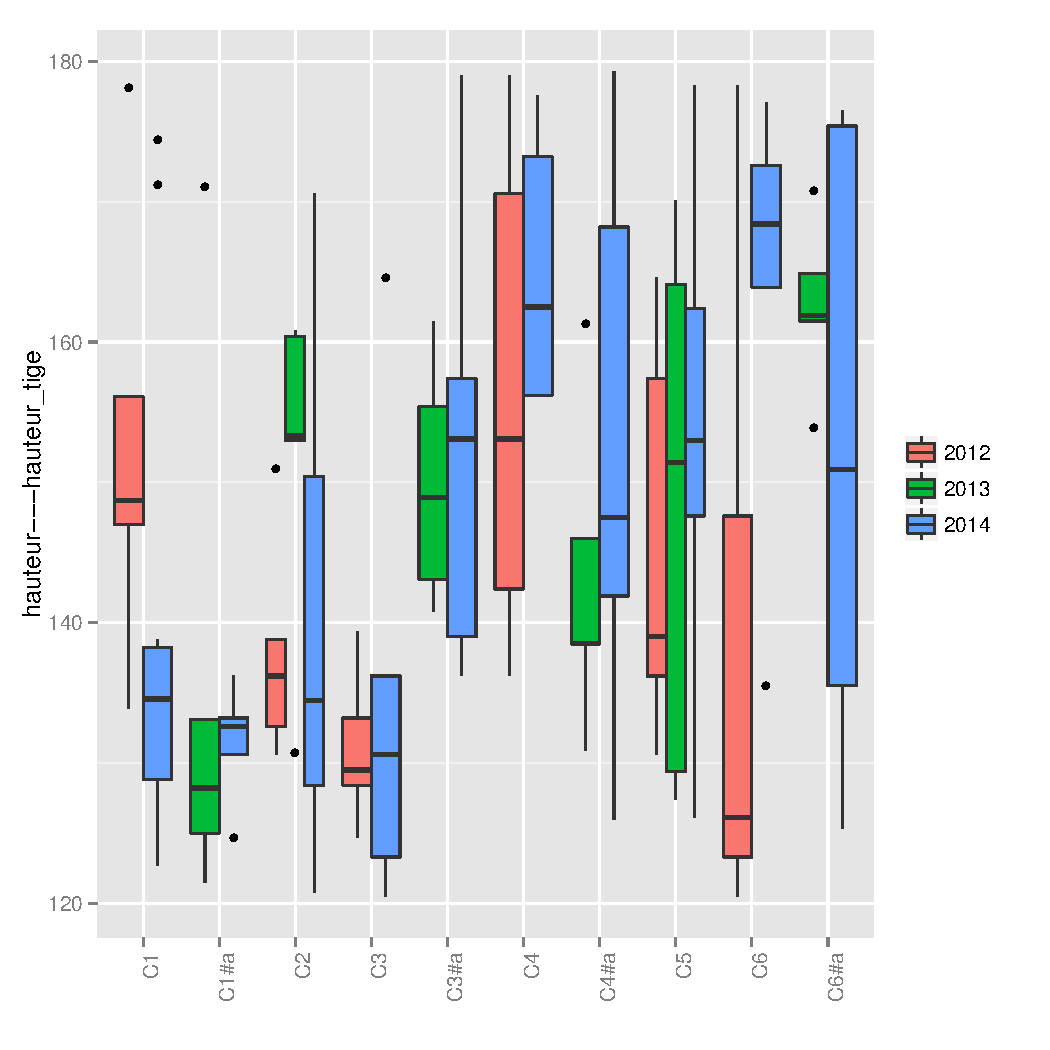
\includegraphics[width=.6\textwidth]{figures/shinemas2R_unnamed-chunk-72-1} 

}



\end{knitrout}
\\
\texttt{p2}\\
\begin{knitrout}
\definecolor{shadecolor}{rgb}{0.969, 0.969, 0.969}\color{fgcolor}

{\centering 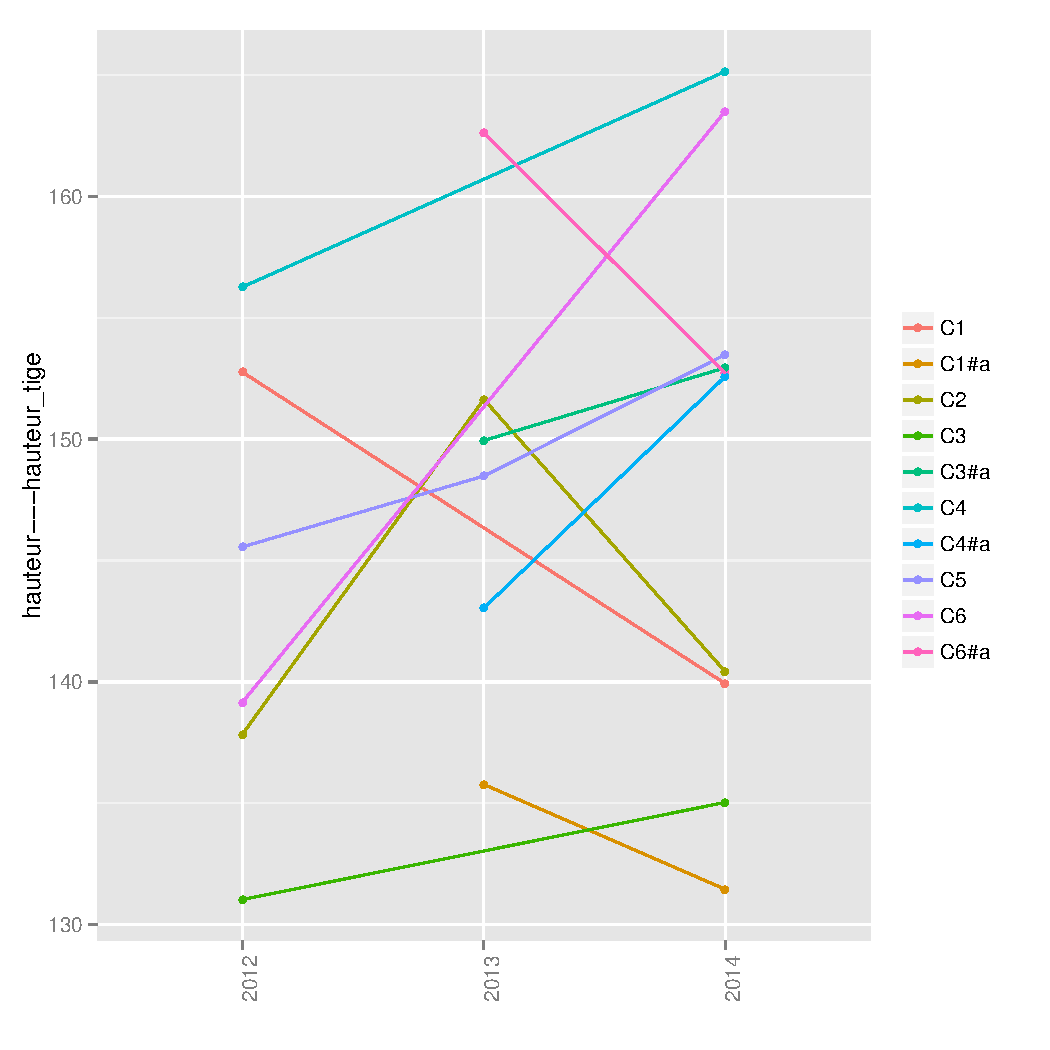
\includegraphics[width=.8\textwidth]{figures/shinemas2R_unnamed-chunk-73-1} 

}



\end{knitrout}
\\
\end{tabular}
\end{center}

\item Custom arguments

Arguments can be customed related to network plots (Table \ref{custom.network}).

\end{itemize}


\item pies on network

\begin{itemize}

\item Default arguments

\texttt{get.data} is called to get the coordinates data.

\begin{knitrout}
\definecolor{shadecolor}{rgb}{0.969, 0.969, 0.969}\color{fgcolor}\begin{kframe}
\begin{alltt}
\hlcom{#data_classic_ter = get.data(}
\hlcom{#	db_user = info_db$db_user, db_host = info_db$db_host, # db infos}
\hlcom{#	db_name = info_db$db_name, db_password = info_db$db_password, # db infos}
\hlcom{#	query.type = "data-classic", # data-classic query}
\hlcom{#	germplasm.in = "Rouge-du-Roc", # germplasm to keep}
\hlcom{#	person.in = c("RAB", "CHD", "JSG"), # person to keep}
\hlcom{#	filter.on = "father-son", # filters on father AND son}
\hlcom{#	data.type = "relation", # data linked to relation between seed-lots}
\hlcom{#	variable = vec_variables, # the variables to display}
\hlcom{#	project.in = "PPB" # the project }
\hlcom{#)}

\hlcom{#data_classic_ter = encrypt.data(data_classic_ter)}

\hlcom{#load("./data/data_classic_ter.RData")}

\hlcom{#pm = get.ggplot(}
\hlcom{#	data_classic_ter, }
\hlcom{#	ggplot.type = "data-pie.on.map", }
\hlcom{#	vec_variables = "spike_weight---spike_weight"}
\hlcom{#	)}

\hlkwd{load}\hlstd{(}\hlstr{"./data/pm.RData"}\hlstd{)}

\hlkwd{names}\hlstd{(pm}\hlopt{$}\hlstd{`data-pie.on.map`)}
\end{alltt}
\begin{verbatim}
## [1] "spike_weight---spike_weight"
\end{verbatim}
\end{kframe}
\end{knitrout}

\begin{knitrout}
\definecolor{shadecolor}{rgb}{0.969, 0.969, 0.969}\color{fgcolor}\begin{kframe}
\begin{alltt}
\hlstd{pm}\hlopt{$}\hlstd{`data-pie.on.map`}\hlopt{$}\hlstd{`spike_weight---spike_weight`}\hlopt{$}\hlstd{`map-[2013]`}
\end{alltt}
\end{kframe}

{\centering 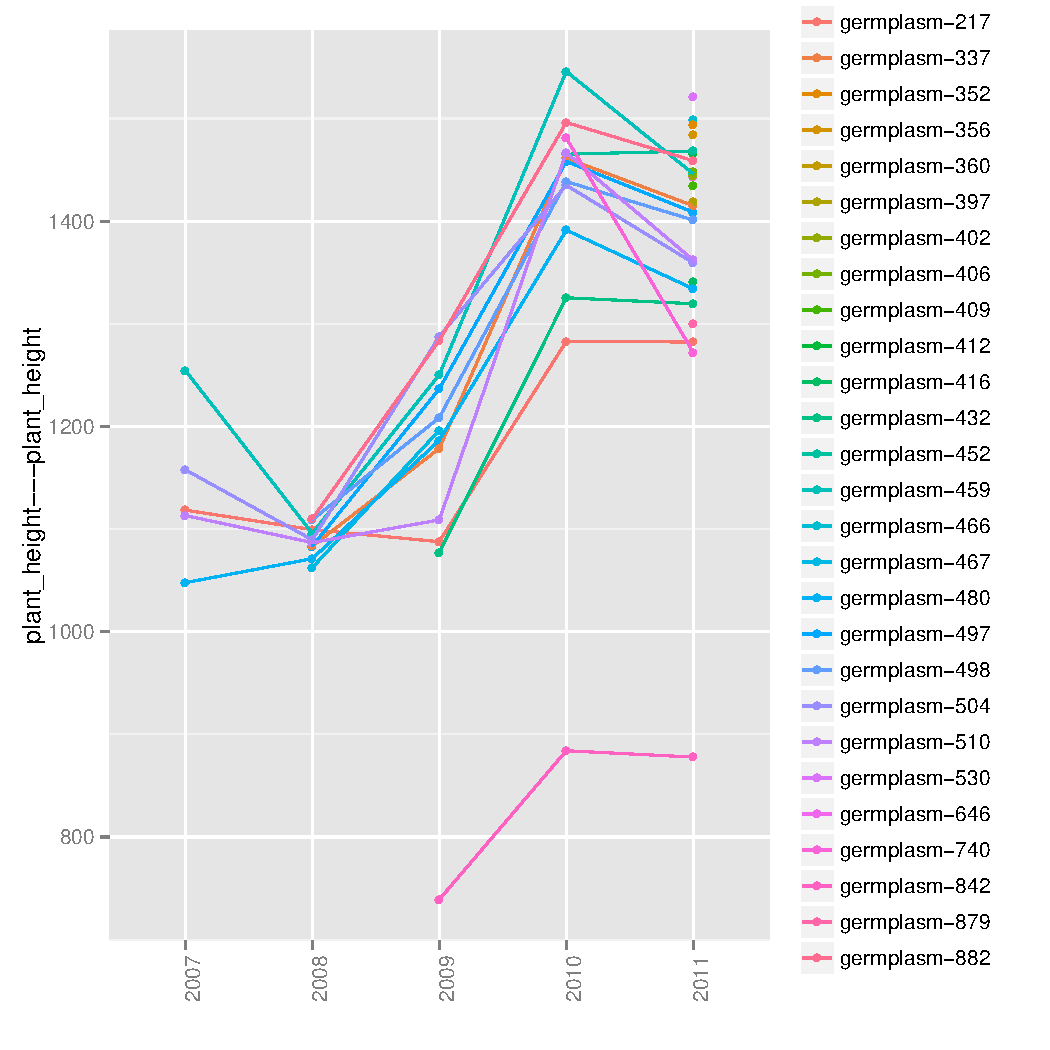
\includegraphics[width=.8\textwidth]{figures/shinemas2R_unnamed-chunk-75-1} 

}



\end{knitrout}

\item Custom arguments

Arguments can be customed related to map plots (Table \ref{custom.map}).

For \texttt{data-pie.on.map}, it is also possible to choose \texttt{x.axis} in order to get a map for each \texttt{year} or each \texttt{germplasm}.

In the example, as \texttt{data\_classic} is done on one germplasm (Rouge du Roc), \texttt{x.axis = year} has been chosen (default argument).

\end{itemize}

\end{itemize}

\subsubsection{ggplots for \texttt{data-S} }

\begin{knitrout}
\definecolor{shadecolor}{rgb}{0.969, 0.969, 0.969}\color{fgcolor}\begin{kframe}
\begin{alltt}
\hlstd{default_data_S_ggplot} \hlkwb{=} \hlkwd{get.ggplot}\hlstd{(}
        \hlstd{data_S,}
        \hlkwc{vec_variables} \hlstd{= vec_variables,}
        \hlkwc{nb_parameters_per_plot_x.axis} \hlstd{=} \hlnum{5}
        \hlstd{)}
\end{alltt}


{\ttfamily\noindent\itshape\color{messagecolor}{\#\# As ggplot.type is NULL, ggplot.Type is set to data-barplot, data-boxplot, data-interaction, data-radar, data-biplot\\\#\# As ggplot.type is NULL and data come from "{}data-S"{} or "{}data-SR"{}, ggplot.type is set to "{}data-barplot"{}, "{}data-boxplot"{}, "{}data-interaction"{}.\\\#\# With "{}data-S"{} and "{}data-SR"{}, in.col and x.axis are set automaticaly.}}\begin{verbatim}
## [1] "A Virer quand les données seront propres dans get.data"
## [1] "A Virer quand les données seront propres dans get.data"
## [1] "A Virer quand les données seront propres dans get.data"
\end{verbatim}
\end{kframe}
\end{knitrout}

By default, the following plots are done with \texttt{x.axis} and \texttt{in.col} by default (you can not change it):

\begin{knitrout}
\definecolor{shadecolor}{rgb}{0.969, 0.969, 0.969}\color{fgcolor}\begin{kframe}
\begin{alltt}
\hlkwd{names}\hlstd{(default_data_S_ggplot)}
\end{alltt}
\begin{verbatim}
## [1] "data-barplot"     "data-boxplot"     "data-interaction"
\end{verbatim}
\end{kframe}
\end{knitrout}

which correpond to ggplot.type arguments as explained in the previous section.

\begin{knitrout}
\definecolor{shadecolor}{rgb}{0.969, 0.969, 0.969}\color{fgcolor}\begin{kframe}
\begin{alltt}
\hlstd{p_S_sw_bar_all} \hlkwb{=} \hlstd{default_data_S_ggplot}\hlopt{$}\hlstd{`data-barplot`}
\hlstd{p_S_sw_bar} \hlkwb{=} \hlstd{p_S_sw_bar_all}\hlopt{$}\hlstd{`spike_weight---spike_weight`}\hlopt{$}\hlstd{`x.axis-1|in.col-1`}
\hlstd{p_S_sw_bar}
\end{alltt}
\end{kframe}

{\centering 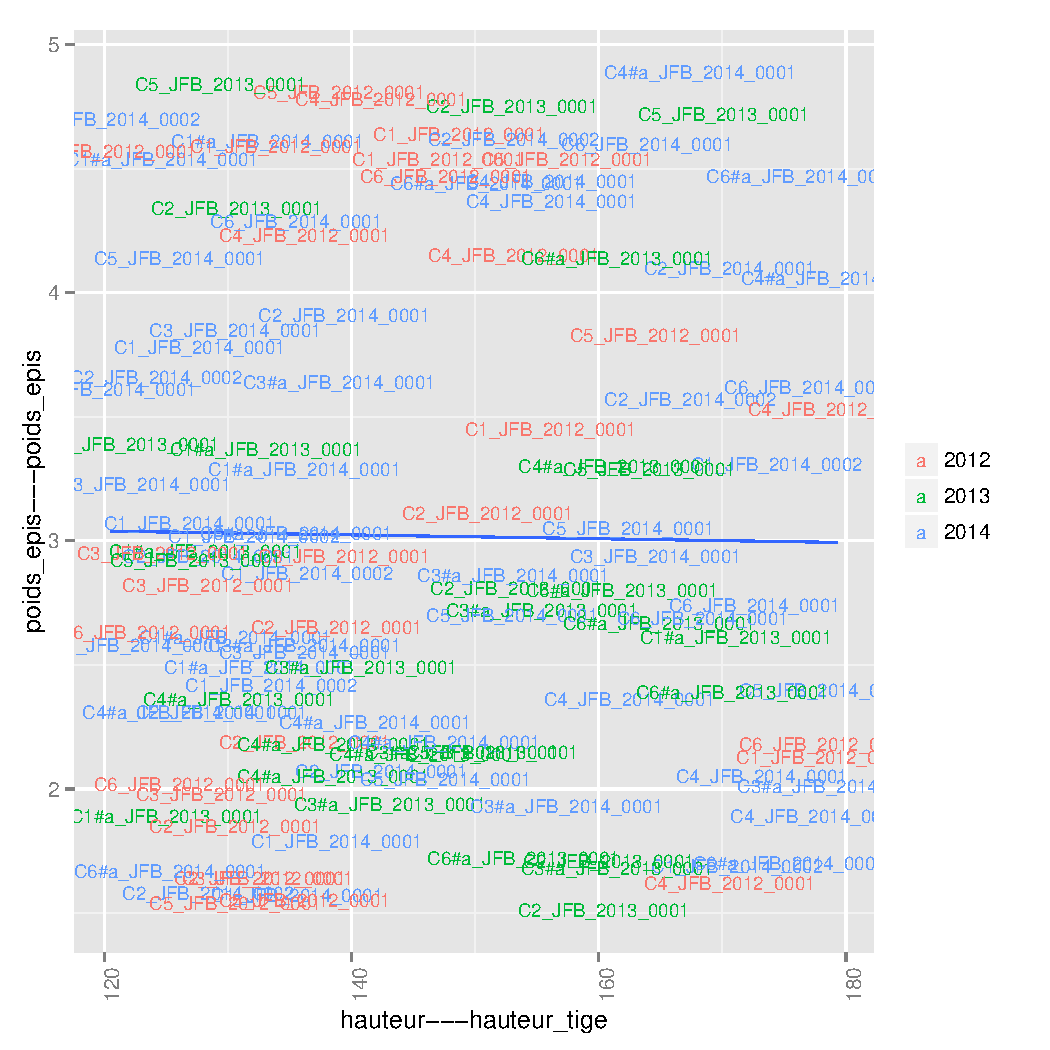
\includegraphics[width=\maxwidth]{figures/shinemas2R_unnamed-chunk-78-1} 

}



\end{knitrout}


\begin{knitrout}
\definecolor{shadecolor}{rgb}{0.969, 0.969, 0.969}\color{fgcolor}\begin{kframe}
\begin{alltt}
\hlstd{p_S_sw_box_all} \hlkwb{=} \hlstd{default_data_S_ggplot}\hlopt{$}\hlstd{`data-boxplot`}
\hlstd{p_S_sw_box} \hlkwb{=} \hlstd{p_S_sw_box_all}\hlopt{$}\hlstd{`spike_weight---spike_weight`}\hlopt{$}\hlstd{`x.axis-1|in.col-1`}
\hlstd{p_S_sw_box}
\end{alltt}
\end{kframe}

{\centering 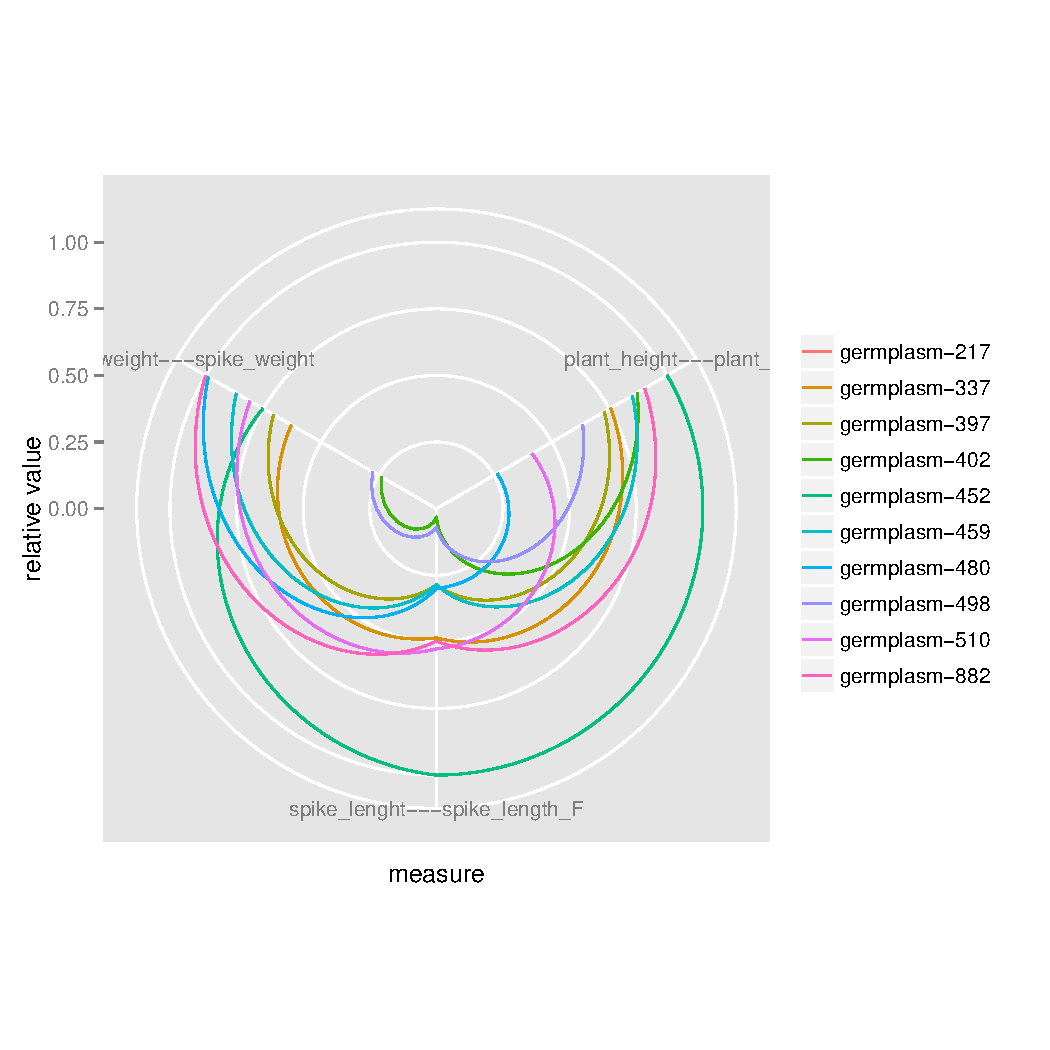
\includegraphics[width=\maxwidth]{figures/shinemas2R_unnamed-chunk-79-1} 

}



\end{knitrout}


\begin{knitrout}
\definecolor{shadecolor}{rgb}{0.969, 0.969, 0.969}\color{fgcolor}\begin{kframe}
\begin{alltt}
\hlstd{p_S_sw_int_all} \hlkwb{=} \hlstd{default_data_S_ggplot}\hlopt{$}\hlstd{`data-interaction`}
\hlstd{p_S_sw_int} \hlkwb{=} \hlstd{p_S_sw_int_all}\hlopt{$}\hlstd{`spike_weight---spike_weight`}\hlopt{$}\hlstd{`x.axis-1|in.col-1`}
\hlstd{p_S_sw_int}
\end{alltt}
\end{kframe}

{\centering 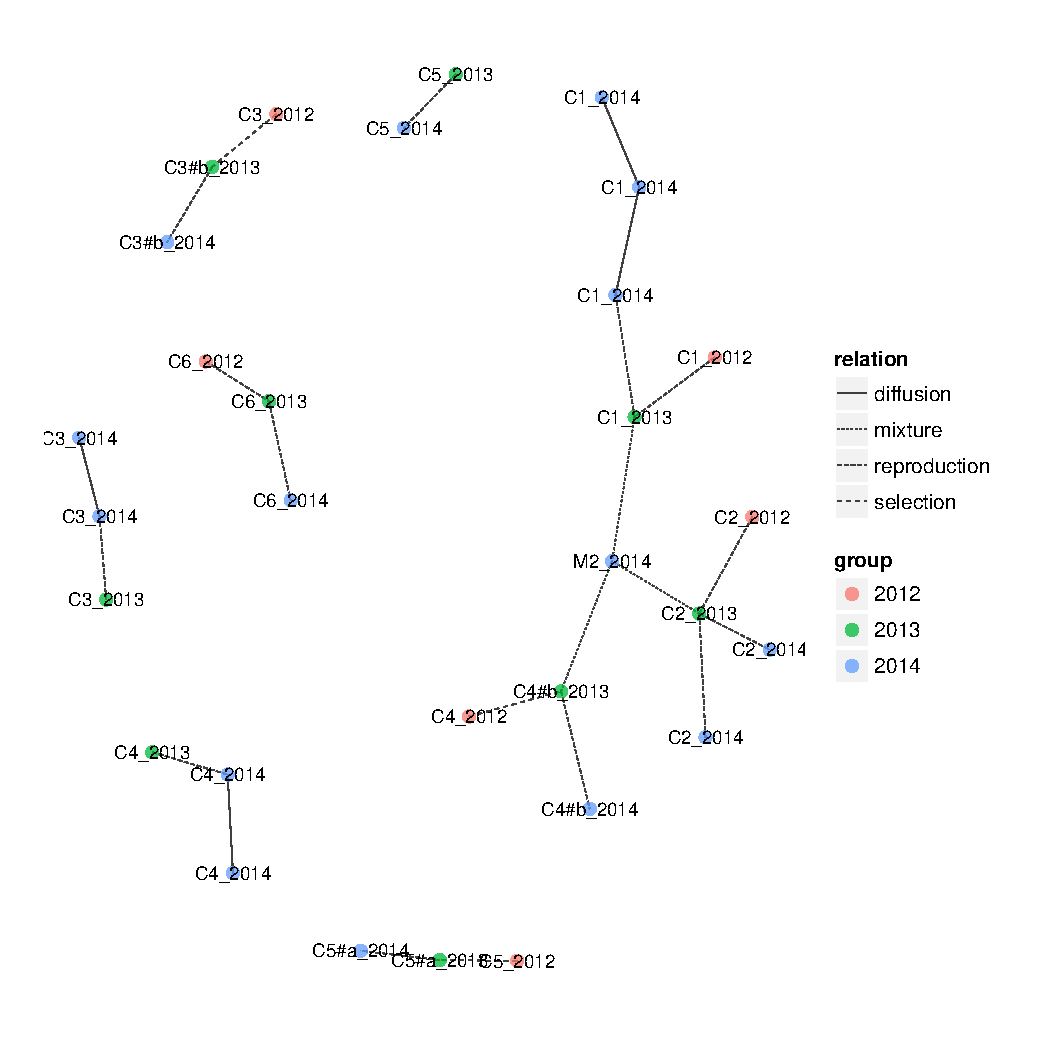
\includegraphics[width=\maxwidth]{figures/shinemas2R_unnamed-chunk-80-1} 

}



\end{knitrout}

It is possible to customize the plots as presented in Table \ref{custom.plot}.

\subsubsection{ggplots for \texttt{data-SR} }

\begin{knitrout}
\definecolor{shadecolor}{rgb}{0.969, 0.969, 0.969}\color{fgcolor}\begin{kframe}
\begin{alltt}
\hlstd{default_data_SR_ggplot} \hlkwb{=} \hlkwd{get.ggplot}\hlstd{(}
        \hlstd{data_SR,}
        \hlkwc{vec_variables} \hlstd{= vec_variables,}
        \hlkwc{nb_parameters_per_plot_x.axis} \hlstd{=} \hlnum{5}
        \hlstd{)}
\end{alltt}


{\ttfamily\noindent\itshape\color{messagecolor}{\#\# As ggplot.type is NULL, ggplot.Type is set to data-barplot, data-boxplot, data-interaction, data-radar, data-biplot\\\#\# As ggplot.type is NULL and data come from "{}data-S"{} or "{}data-SR"{}, ggplot.type is set to "{}data-barplot"{}, "{}data-boxplot"{}, "{}data-interaction"{}.\\\#\# With "{}data-S"{} and "{}data-SR"{}, in.col and x.axis are set automaticaly.}}\begin{verbatim}
## [1] "A Virer quand les données seront propres dans get.data"
## [1] "A Virer quand les données seront propres dans get.data"
## [1] "A Virer quand les données seront propres dans get.data"
\end{verbatim}
\end{kframe}
\end{knitrout}

By default, the following plots are done with \texttt{x.axis} and \texttt{in.col} by default (you can not change it):

\begin{knitrout}
\definecolor{shadecolor}{rgb}{0.969, 0.969, 0.969}\color{fgcolor}\begin{kframe}
\begin{alltt}
\hlkwd{names}\hlstd{(default_data_SR_ggplot)}
\end{alltt}
\begin{verbatim}
## [1] "data-barplot"     "data-boxplot"     "data-interaction"
\end{verbatim}
\end{kframe}
\end{knitrout}

which correpond to ggplot.type arguments as explained in the previsou section.

\begin{knitrout}
\definecolor{shadecolor}{rgb}{0.969, 0.969, 0.969}\color{fgcolor}\begin{kframe}
\begin{alltt}
\hlstd{p_SR_sw_bar_all} \hlkwb{=} \hlstd{default_data_S_ggplot}\hlopt{$}\hlstd{`data-barplot`}
\hlstd{p_SR_sw_bar} \hlkwb{=} \hlstd{p_SR_sw_bar_all}\hlopt{$}\hlstd{`spike_weight---spike_weight`}\hlopt{$}\hlstd{`x.axis-1|in.col-1`}
\hlstd{p_SR_sw_bar}
\end{alltt}
\end{kframe}

{\centering 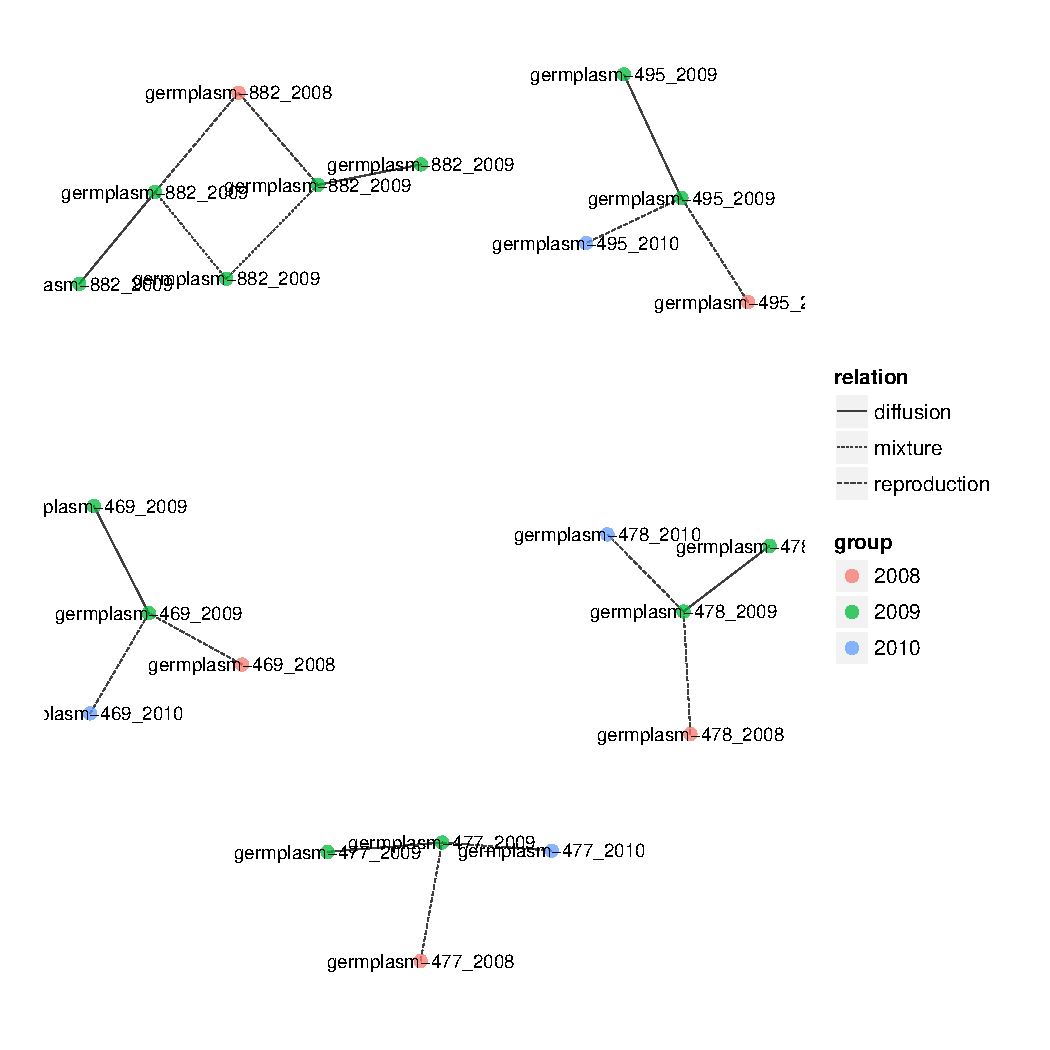
\includegraphics[width=\maxwidth]{figures/shinemas2R_unnamed-chunk-83-1} 

}



\end{knitrout}


\begin{knitrout}
\definecolor{shadecolor}{rgb}{0.969, 0.969, 0.969}\color{fgcolor}\begin{kframe}
\begin{alltt}
\hlstd{p_SR_sw_box_all} \hlkwb{=} \hlstd{default_data_S_ggplot}\hlopt{$}\hlstd{`data-boxplot`}
\hlstd{p_SR_sw_box} \hlkwb{=} \hlstd{p_SR_sw_box_all}\hlopt{$}\hlstd{`spike_weight---spike_weight`}\hlopt{$}\hlstd{`x.axis-1|in.col-1`}
\hlstd{p_SR_sw_box}
\end{alltt}
\end{kframe}

{\centering 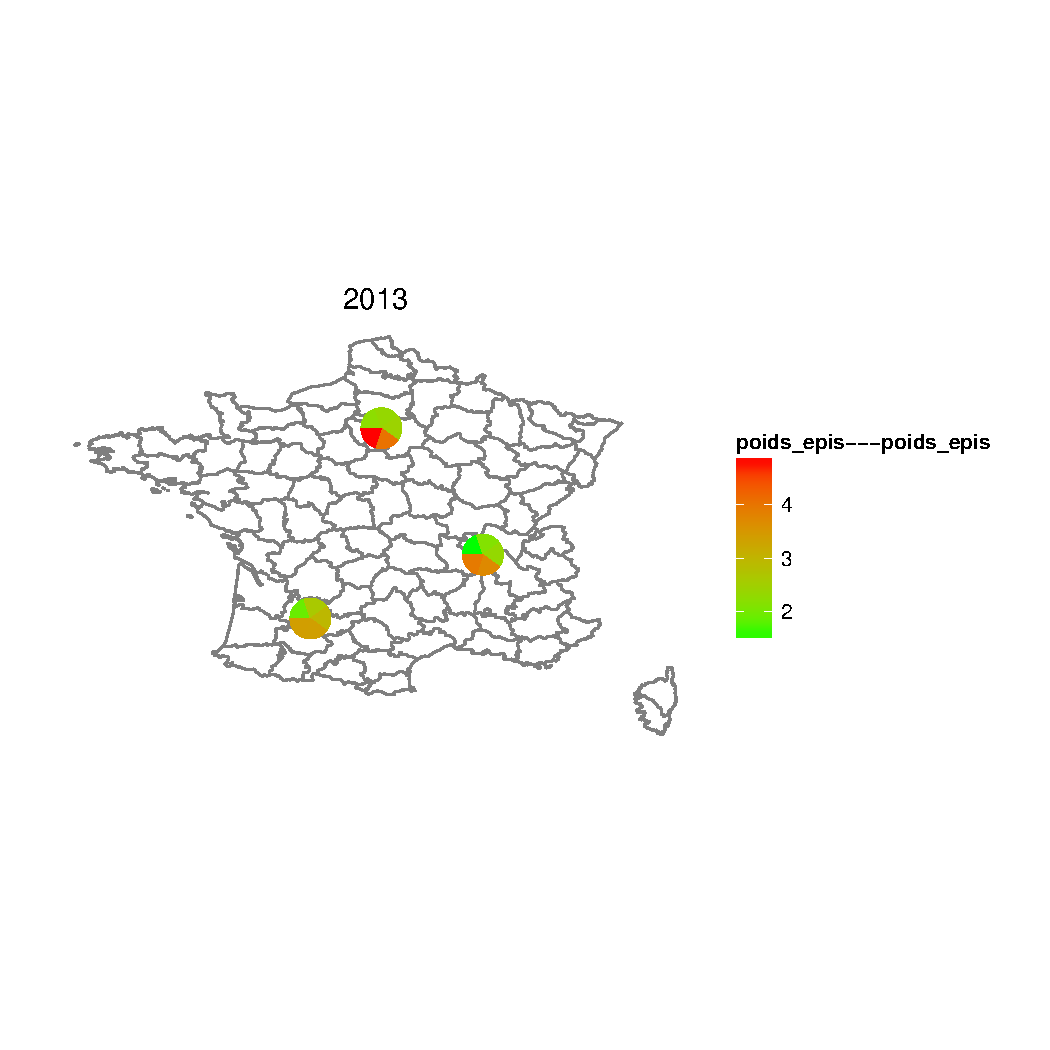
\includegraphics[width=\maxwidth]{figures/shinemas2R_unnamed-chunk-84-1} 

}



\end{knitrout}


\begin{knitrout}
\definecolor{shadecolor}{rgb}{0.969, 0.969, 0.969}\color{fgcolor}\begin{kframe}
\begin{alltt}
\hlstd{p_SR_sw_int_all} \hlkwb{=} \hlstd{default_data_S_ggplot}\hlopt{$}\hlstd{`data-interaction`}
\hlstd{p_SR_sw_int} \hlkwb{=} \hlstd{p_SR_sw_int_all}\hlopt{$}\hlstd{`spike_weight---spike_weight`}\hlopt{$}\hlstd{`x.axis-1|in.col-1`}
\hlstd{p_SR_sw_int}
\end{alltt}
\end{kframe}

{\centering 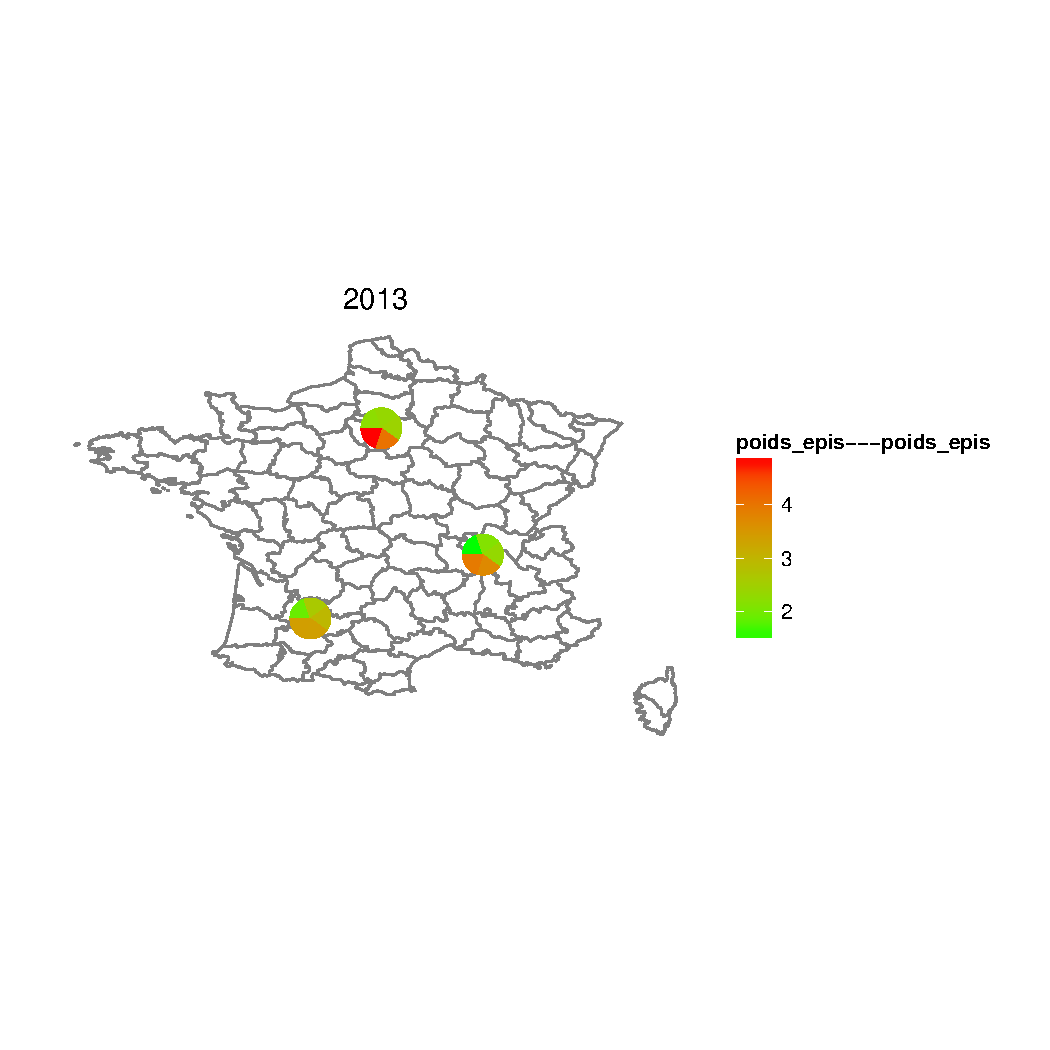
\includegraphics[width=\maxwidth]{figures/shinemas2R_unnamed-chunk-85-1} 

}



\end{knitrout}

It is possible to customize the plots as presented in Table \ref{custom.plot}.


\subsection{Get the tables}

From the data, to get the tables, use the function \texttt{get.table}.
Five types of tables can be display according to \texttt{table.type} argument :

\begin{center}
\begin{tabular}{ll}
\hline
\texttt{table.type} & description \\
\hline

\texttt{"raw"} & display raw data. Useful with text for example \\
\hline

\texttt{"mean"} & display for each variable columns with mean \\
\hline

\texttt{"mean.sd"} & display for each variable columns with mean and standard deviation \\
\hline

\texttt{"mean.sd.cv"} & display for each variable columns with mean, standard deviation and coefficient of variation \\
\hline

\texttt{"summary"} & display \texttt{"Min."}, \texttt{"1st Qu."}, \texttt{"Median"}, \texttt{"3rd Qu."}, \texttt{"Max."} of the data \\
\hline
\end{tabular}
\end{center}

The table always display information with seed-lots on the left side.
For information on relation, you must choose if seed-lots displayed in the table are the son or the father with the argument \texttt{table.on}.
For information on seed-lots, there is no problems.

Then you should set \texttt{vec\_variables} with the variables displayed in the table.

\subsubsection{tables for \texttt{data-classic} }

\begin{itemize}

\item Default arguments

\begin{knitrout}
\definecolor{shadecolor}{rgb}{0.969, 0.969, 0.969}\color{fgcolor}\begin{kframe}
\begin{alltt}
\hlstd{tab_class} \hlkwb{=} \hlkwd{get.table}\hlstd{(}
        \hlstd{data_classic,}
        \hlkwc{table.type} \hlstd{=} \hlstr{"raw"}\hlstd{,}
        \hlkwc{vec_variables} \hlstd{= vec_variables}
        \hlstd{)}
\end{alltt}
\end{kframe}
\end{knitrout}


the function returns a list with two elements:
\begin{knitrout}
\definecolor{shadecolor}{rgb}{0.969, 0.969, 0.969}\color{fgcolor}\begin{kframe}
\begin{alltt}
\hlkwd{names}\hlstd{(tab_class)}
\end{alltt}
\begin{verbatim}
## [1] "duplicated_infos"     "not_duplicated_infos"
\end{verbatim}
\end{kframe}
\end{knitrout}

\begin{itemize}
\item \texttt{"duplicated\_infos"}: lists of two elements with seed-lots involved and variable values
\begin{knitrout}
\definecolor{shadecolor}{rgb}{0.969, 0.969, 0.969}\color{fgcolor}\begin{kframe}
\begin{alltt}
\hlstd{tab_class}\hlopt{$}\hlstd{duplicated_infos}\hlopt{$}\hlstd{`set-1`}
\end{alltt}
\begin{verbatim}
## NULL
\end{verbatim}
\end{kframe}
\end{knitrout}

It is \texttt{NULL} as there are no duplicated information here.

An example with duplicated information:

\begin{knitrout}
\definecolor{shadecolor}{rgb}{0.969, 0.969, 0.969}\color{fgcolor}\begin{kframe}
\begin{alltt}
\hlcom{#data_classic_4 = get.data(}
\hlcom{#	db_user = info_db$db_user, db_host = info_db$db_host, # db infos}
\hlcom{#	db_name = info_db$db_name, db_password = info_db$db_password, # db infos}
\hlcom{#	query.type = "data-classic", # data-classic query}
\hlcom{#	person.in = "RAB", # person to keep}
\hlcom{#	filter.on = "father-son", # filters on father AND son}
\hlcom{#	data.type = "relation", # data linked to relation between seed-lots}
\hlcom{#	variable = "sowing_practices", # the variables to display}
\hlcom{#	project.in = "PPB" # the project}
\hlcom{#	)}

\hlcom{# data_classic_4 = encrypt.data(data_classic_4)}

\hlkwd{load}\hlstd{(}\hlstr{"./data/data_classic_4.RData"}\hlstd{)}

\hlstd{tab_class_4} \hlkwb{=} \hlkwd{get.table}\hlstd{(}
        \hlstd{data_classic_4,}
        \hlkwc{table.type} \hlstd{=} \hlstr{"raw"}\hlstd{,}
        \hlkwc{vec_variables} \hlstd{=} \hlstr{"sowing_practices---sowing_notice_sowing_practices"}
        \hlstd{)}
\end{alltt}
\end{kframe}
\end{knitrout}

The information is divided in two:
\begin{knitrout}
\definecolor{shadecolor}{rgb}{0.969, 0.969, 0.969}\color{fgcolor}\begin{kframe}
\begin{alltt}
\hlkwd{names}\hlstd{(tab_class_4}\hlopt{$}\hlstd{duplicated_infos}\hlopt{$}\hlstd{`set-1`)}
\end{alltt}
\begin{verbatim}
## [1] "duplicated_infos_seed-lots" "duplicated_infos_variables"
\end{verbatim}
\end{kframe}
\end{knitrout}

The seed-lots that are concerned.
By default \texttt{col\_to\_display = c("person", "germplasm", "year", "block", "X", "Y")}, therefore, the information is under the form : 
\texttt{person-germplasm-year-block-X-Y}.
\begin{knitrout}
\definecolor{shadecolor}{rgb}{0.969, 0.969, 0.969}\color{fgcolor}\begin{kframe}
\begin{alltt}
\hlstd{tab_class_4}\hlopt{$}\hlstd{duplicated_infos}\hlopt{$}\hlstd{`set-1`}\hlopt{$}\hlstd{`duplicated_infos_seed-lots`}
\end{alltt}
\begin{verbatim}
##                                                                                                                                                                                                                                                                                                                                                                                                                                                                                                                                                                                                                                                                                                                                                                                                                                                                                                                                                                                                                                                                                                                                                                                                                                                                                                                                                                                                                                                                                                                                                                                                                                                                                                                                                                                                                                                                                                                                                                                                                                                                                                                                                                                                                                                                                                                                                                                                                                                                                                                                                                                                                                                                                                                                                                                                                                                                                                                                                                                                                                                                                                                                                                                                                                                                                                                                                                                                                                                                                                                                                                                                                                                                                                                                                                                                                                                                                                                                                                                                                                                                                                                                                                                                                                                                                                                                                                                                                                                                                                                                                                                                                                                                                                                                                                                                       seed-lots
## 1 person-106-germplasm-337-2010-1-A-13, person-106-germplasm-337-2011-2-B-8, person-106-germplasm-337-2011-2-B-9, person-106-germplasm-337-2008-1-NA-NA, person-106-germplasm-337-2009-2-NA-NA, person-106-germplasm-337-2009-1-NA-1, person-106-germplasm-337-2009-1-NA-2, person-106-germplasm-337-2010-2-A-2, person-106-germplasm-337-2010-1-A-12, person-106-germplasm-337-2011-1-C-2, person-106-germplasm-337-2011-2-B-7, person-106-germplasm-352-2011-1-E-1, person-106-germplasm-356-2011-1-E-5, person-106-germplasm-360-2011-2-C-9, person-106-germplasm-398-2009-3-NA-NA, person-106-germplasm-399-2009-3-NA-NA, person-106-germplasm-400-2009-3-NA-NA, person-106-germplasm-401-2009-3-NA-NA, person-106-germplasm-397-2011-2-B-6, person-106-germplasm-403-2009-3-NA-NA, person-106-germplasm-404-2009-3-NA-NA, person-106-germplasm-405-2009-3-NA-NA, person-106-germplasm-402-2011-1-E-4, person-106-germplasm-407-2009-3-NA-NA, person-106-germplasm-408-2009-3-NA-NA, person-106-germplasm-406-2011-1-B-1, person-106-germplasm-410-2009-3-NA-NA, person-106-germplasm-411-2009-3-NA-NA, person-106-germplasm-409-2011-1-C-1, person-106-germplasm-413-2009-3-NA-NA, person-106-germplasm-414-2009-3-NA-NA, person-106-germplasm-415-2009-3-NA-NA, person-106-germplasm-412-2011-2-A-6, person-106-germplasm-417-2009-3-NA-NA, person-106-germplasm-418-2009-3-NA-NA, person-106-germplasm-419-2009-3-NA-NA, person-106-germplasm-416-2011-1-A-2, person-106-germplasm-217-2010-1-A-19, person-106-germplasm-217-2011-2-C-7, person-106-germplasm-217-2011-2-C-8, person-106-germplasm-217-2008-1-NA-NA, person-106-germplasm-217-2009-1-NA-NA, person-106-germplasm-217-2010-1-A-16, person-106-germplasm-217-2011-2-E-7, person-106-germplasm-432-2010-1-A-20, person-106-germplasm-432-2011-2-D-6, person-106-germplasm-432-2009-2-NA-1, person-106-germplasm-432-2009-2-NA-2, person-106-germplasm-432-2009-1-NA-NA, person-106-germplasm-432-2010-2-A-3, person-106-germplasm-432-2010-1-A-17, person-106-germplasm-432-2011-1-D-5, person-106-germplasm-432-2011-2-A-9, person-106-germplasm-432-2009-2-NA-NA, person-106-germplasm-432-2010-2-A-1, person-106-germplasm-432-2011-1-C-3, person-106-germplasm-432-2011-2-D-7, person-106-germplasm-452-2011-2-E-9, person-106-germplasm-452-2010-1-A-25, person-106-germplasm-452-2011-2-E-8, person-106-germplasm-459-2010-1-A-15, person-106-germplasm-459-2011-2-A-7, person-106-germplasm-459-2011-2-A-8, person-106-germplasm-459-2008-1-NA-NA, person-106-germplasm-459-2009-2-NA-NA, person-106-germplasm-459-2010-2-A-11, person-106-germplasm-459-2011-2-C-10, person-106-germplasm-466-2011-1-D-4, person-106-germplasm-467-2008-1-NA-NA, person-106-germplasm-467-2009-2-NA-NA, person-106-germplasm-480-2010-2-A-6, person-106-germplasm-480-2011-1-C-4, person-106-germplasm-480-2011-1-C-5, person-106-germplasm-480-2008-1-NA-NA, person-106-germplasm-480-2009-1-NA-NA, person-106-germplasm-480-2010-2-A-4, person-106-germplasm-480-2011-2-D-10, person-106-germplasm-498-2011-1-A-5, person-106-germplasm-498-2008-1-NA-NA, person-106-germplasm-498-2009-2-NA-NA, person-106-germplasm-498-2010-1-A-23, person-106-germplasm-498-2011-1-A-4, person-106-germplasm-504-2008-1-NA-NA, person-106-germplasm-504-2009-1-NA-NA, person-106-germplasm-504-2010-1-A-22, person-106-germplasm-504-2011-1-A-3, person-106-germplasm-497-2008-1-NA-NA, person-106-germplasm-497-2009-2-NA-NA, person-106-germplasm-497-2010-1-A-14, person-106-germplasm-497-2011-1-B-5, person-106-germplasm-510-2010-2-A-8, person-106-germplasm-510-2011-1-B-2, person-106-germplasm-510-2011-1-B-3, person-106-germplasm-510-2008-1-NA-NA, person-106-germplasm-510-2009-1-NA-NA, person-106-germplasm-510-2010-2-A-5, person-106-germplasm-510-2011-2-B-10, person-106-germplasm-530-2011-2-D-9, person-106-germplasm-646-2011-1-B-4, person-106-germplasm-646-2011-2-D-8, person-106-germplasm-740-2010-2-A-10, person-106-germplasm-740-2011-1-E-2, person-106-germplasm-842-2009-2-NA-NA, person-106-germplasm-842-2009-1-NA-NA, person-106-germplasm-842-2010-2-A-9, person-106-germplasm-842-2010-1-A-24, person-106-germplasm-842-2011-1-E-3, person-106-germplasm-842-2011-2-C-6, person-106-germplasm-879-2011-1-D-1, person-106-germplasm-879-2011-2-E-6, person-106-germplasm-879-2011-2-A-10, person-106-germplasm-882-2011-1-D-2, person-106-germplasm-882-2011-1-D-3, person-106-germplasm-882-2008-1-NA-1, person-106-germplasm-882-2008-1-NA-2, person-106-germplasm-882-2008-1-NA-3, person-106-germplasm-882-2009-2-NA-NA, person-106-germplasm-882-2009-1-NA-NA, person-106-germplasm-882-2010-2-A-7, person-106-germplasm-882-2010-1-A-18, person-106-germplasm-882-2011-1-A-1, person-106-germplasm-882-2011-2-E-10
\end{verbatim}
\end{kframe}
\end{knitrout}

And the data linked to these seed lots:
\begin{knitrout}
\definecolor{shadecolor}{rgb}{0.969, 0.969, 0.969}\color{fgcolor}\begin{kframe}
\begin{alltt}
\hlstd{tab_class_4}\hlopt{$}\hlstd{duplicated_infos}\hlopt{$}\hlstd{`set-1`}\hlopt{$}\hlstd{`duplicated_infos_variables`}
\end{alltt}
\begin{verbatim}
##   sowing_practices---sowing_notice_sowing_practices
## 1                                             volée
\end{verbatim}
\end{kframe}
\end{knitrout}


\item \texttt{"not\_duplicated\_infos"}: a list with the table of non duplicated information
\begin{knitrout}
\definecolor{shadecolor}{rgb}{0.969, 0.969, 0.969}\color{fgcolor}\begin{kframe}
\begin{alltt}
\hlkwd{dim}\hlstd{(tab_class}\hlopt{$}\hlstd{not_duplicated_infos}\hlopt{$}\hlstd{`set-1`)}
\end{alltt}
\begin{verbatim}
## [1] 3244   10
\end{verbatim}
\end{kframe}
\end{knitrout}
\end{itemize}

Note that the threshold up to which the information are duplicated or not is tuned with the argument \texttt{nb\_duplicated\_rows} (see Custom arguments).


Instead of raw information, some statistics may be useful, for example,
\begin{knitrout}
\definecolor{shadecolor}{rgb}{0.969, 0.969, 0.969}\color{fgcolor}\begin{kframe}
\begin{alltt}
\hlstd{tab_class} \hlkwb{=} \hlkwd{get.table}\hlstd{(}
        \hlstd{data_classic,}
        \hlkwc{table.type} \hlstd{=} \hlstr{"mean.sd.cv"}\hlstd{,}
        \hlkwc{vec_variables} \hlstd{= vec_variables}
        \hlstd{)}
\hlkwd{names}\hlstd{(tab_class}\hlopt{$}\hlstd{not_duplicated_infos)}
\end{alltt}
\begin{verbatim}
## [1] "set-1"
\end{verbatim}
\begin{alltt}
\hlkwd{colnames}\hlstd{(tab_class}\hlopt{$}\hlstd{not_duplicated_infos}\hlopt{$}\hlstd{`set-1`)}
\end{alltt}
\begin{verbatim}
##  [1] "person"                            
##  [2] "germplasm"                         
##  [3] "year"                              
##  [4] "block"                             
##  [5] "X"                                 
##  [6] "Y"                                 
##  [7] "spike_weight---spike_weight mean"  
##  [8] "spike_weight---spike_weight sd"    
##  [9] "spike_weight---spike_weight cv"    
## [10] "plant_height---plant_height mean"  
## [11] "plant_height---plant_height sd"    
## [12] "plant_height---plant_height cv"    
## [13] "spike_lenght---spike_length_F mean"
## [14] "spike_lenght---spike_length_F sd"  
## [15] "spike_lenght---spike_length_F cv"  
## [16] "spike_lenght---spike_lenght mean"  
## [17] "spike_lenght---spike_lenght sd"    
## [18] "spike_lenght---spike_lenght cv"
\end{verbatim}
\begin{alltt}
\hlkwd{dim}\hlstd{(tab_class}\hlopt{$}\hlstd{not_duplicated_infos}\hlopt{$}\hlstd{`set-1`)}
\end{alltt}
\begin{verbatim}
## [1] 111  18
\end{verbatim}
\end{kframe}
\end{knitrout}



\item Custom arguments

The following arguments can be customized:


\begin{center}
\begin{table}[H]
\begin{tabular}{ p{.2\textwidth} p{.2\textwidth} p{.5\textwidth}}
\hline
argument & default value & description \\
\hline

\texttt{nb\_row} & \texttt{NULL} & the number of rows in the table \\
\hline

\texttt{nb\_col} & \texttt{NULL} & the number of columns for variable in the table. \texttt{col\_to\_display} remains fixed. \\
\hline

\texttt{nb\_duplicated\_rows} & \texttt{NULL} & minimum number of duplicated rows for each variable of a table up to which the information is put in only one row. \\
\hline

\texttt{col\_to\_display} & \texttt{c("person", "germplasm", "year", "block", "X", "Y")} & columns to display in the table. It can be a vector with \texttt{"person"}, \texttt{"year"}, \texttt{"germplasm"}, \texttt{"block"}, \texttt{"X"} and \texttt{"Y"}. If \texttt{NULL}, none of these columns are displayed. The variables follow these columns. 
For \texttt{"data-S"} and \texttt{"data-SR"} type, the column \texttt{"expe"} and \texttt{"sl\_statut"} are added by default. \\
\hline

\texttt{invert\_row\_col} & \texttt{FALSE} & if \texttt{TRUE}, invert row and col in the table. This is possible only for \texttt{col\_to\_display = NULL}. \\
\hline
\end{tabular}
\caption{Possible arguments to custom \texttt{get.table}.}
\label{custom.table}
\end{table}
\end{center}


\end{itemize}

For examples,

\begin{knitrout}
\definecolor{shadecolor}{rgb}{0.969, 0.969, 0.969}\color{fgcolor}\begin{kframe}
\begin{alltt}
\hlstd{tab_class} \hlkwb{=} \hlkwd{get.table}\hlstd{(}
        \hlstd{data_classic,}
        \hlkwc{table.type} \hlstd{=} \hlstr{"mean.sd.cv"}\hlstd{,}
        \hlkwc{vec_variables} \hlstd{= vec_variables,}
        \hlkwc{nb_row} \hlstd{=} \hlnum{30}
        \hlstd{)}
\hlkwd{names}\hlstd{(tab_class}\hlopt{$}\hlstd{not_duplicated_infos)}
\end{alltt}
\begin{verbatim}
## [1] "set-1" "set-2" "set-3" "set-4"
\end{verbatim}
\end{kframe}
\end{knitrout}

The information is split into several tables with at least 30 rows.

\begin{knitrout}
\definecolor{shadecolor}{rgb}{0.969, 0.969, 0.969}\color{fgcolor}\begin{kframe}
\begin{alltt}
\hlkwd{dim}\hlstd{(tab_class}\hlopt{$}\hlstd{not_duplicated_infos}\hlopt{$}\hlstd{`set-1`)}
\end{alltt}
\begin{verbatim}
## [1] 30 18
\end{verbatim}
\end{kframe}
\end{knitrout}


\subsubsection{tables for \texttt{data-S} and \texttt{data-SR}}
Tables are the same than for \texttt{classic-data}, there is just the column \texttt{"expe"} and \texttt{"sl\_statut"} added by default.

For example,
\begin{knitrout}
\definecolor{shadecolor}{rgb}{0.969, 0.969, 0.969}\color{fgcolor}\begin{kframe}
\begin{alltt}
\hlstd{tab_S_msc} \hlkwb{=} \hlkwd{get.table}\hlstd{(}
        \hlstd{data_S,}
        \hlkwc{table.type} \hlstd{=} \hlstr{"mean.sd.cv"}\hlstd{,}
        \hlkwc{vec_variables} \hlstd{= vec_variables,}
        \hlkwc{nb_col} \hlstd{=} \hlnum{3} \hlcom{# Otherwise, the table is too large}
        \hlstd{)}

\hlkwd{colnames}\hlstd{(tab_S_msc}\hlopt{$}\hlstd{not_duplicated_infos}\hlopt{$}\hlstd{`set-1`)}
\end{alltt}
\begin{verbatim}
##  [1] "person"                          
##  [2] "germplasm"                       
##  [3] "year"                            
##  [4] "block"                           
##  [5] "X"                               
##  [6] "Y"                               
##  [7] "expe"                            
##  [8] "sl_statut"                       
##  [9] "plant_height---plant_height mean"
## [10] "plant_height---plant_height sd"  
## [11] "plant_height---plant_height cv"
\end{verbatim}
\end{kframe}
\end{knitrout}


It is possible to customize the tables as presented in Table \ref{custom.table}.


%\section{Set of \sl}

%\subsection{\texttt{query.type = "SL.mix"}}

%\subsection{\texttt{query.type = "cross"}}


% parler de fuse g s et correlated var pour plot et table

% Faire des exemples avec PPBstats, FactoMineR, etc ? A faire plutôt dans PPBformations ?!?

\newpage


\section{pdf compilation with \LaTeX}
\label{pdf}

\texttt{get.pdf} aggregates texts and outputs from \texttt{get.ggplot} and \texttt{get.table}.
This is particularly useful in participatory research to give feedback to stackholders such as farmers.

\texttt{get.pdf} creates a \texttt{.tex} file that is compiled into a \texttt{.pdf} file.
You need to install \LaTeX~and the following packages : \texttt{longtable}, \texttt{lscape}, \texttt{graphicx}, \texttt{pdfpages}, \texttt{float}, \texttt{hyperref} and \texttt{fancyhdr}. 
To download LaTeX, go to \url{http://latex-project.org/ftp.html}.


\subsection{Philosophy of \texttt{get.pdf} }

The idea of \texttt{get.pdf} is to create a list (\texttt{LaTeX\_body} argument) with several elements that can be:

\begin{itemize}
\item \texttt{"titlepage"} : a list containing the following elements :
	\begin{itemize}
	\item \texttt{"title"} : the title of the document. Nothing by default.
	\item \texttt{"authors"} : the authors of the document. Nothing by default.
	\item \texttt{"email"} : the corresponding email. Nothing by default.
	\item \texttt{"date"} : the date of the document. Nothing by default.
	\end{itemize}

\item \texttt{"tableofcontents"} : if \texttt{TRUE}, a table of content is display.

\item \texttt{"chapter"} : name of a chapter

\item \texttt{"section"} : name of a section

\item \texttt{"subsection"} : name of a subsection

\item \texttt{"subsubsection"} : name of a subsubsection

\item \texttt{"text"} : text to add

\item \texttt{"includepdf"} : path of a .pdf to include

\item \texttt{"input"} : path of a .tex to insert

\item \texttt{"table"} : a list containing the following elements :
	\begin{itemize}
	\item \texttt{"content"} : output from \texttt{get.table}
	\item \texttt{"caption"} : caption of the table
	\item \texttt{"landscape"} : If \texttt{TRUE}, the table is in landscape. \texttt{FALSE} by default.
	\item \texttt{"display.rownames"} : If \texttt{TRUE}, display the row names of the table. \texttt{FALSE} by default.
	\end{itemize}

\item \texttt{"figure"} : a list containing the following elements :
	\begin{itemize}
	\item \texttt{"content"} : output from \texttt{get.ggplot}
	\item \texttt{"caption"} : caption of the figure
	\item \texttt{"layout"} : the layout of the plots. It is a matrix under the form \texttt{layout = matrix(c(1:4), ncol = 2, nrow = 2)}. It is \texttt{layout = matrix(1, ncol = 1, nrow= 1)} by default.
	\item \texttt{"width"} : width of the figure in textwidth unit. 1 means as width as the text. It is 1 by default.
	\item \texttt{"landscape"} : If \texttt{TRUE}, the figure is in landscape. \texttt{FALSE} by default.
	\end{itemize}

\end{itemize}


The elements of this list will be in the same order in the final pdf.

You do not have to know \LaTeX. \texttt{get.pdf} uses it for you.
Nevertheless, if you use \LaTeX~you'll be able to customize the \texttt{.pdf} document by creating the tex structure of the document (\texttt{LaTeX\_head} argument).
It is also possible to add specific tex files (\texttt{input} element of \texttt{LaTeX\_body} argument).
If you use \LaTeX~macro, do not forget to use the escape mode (Table \ref{macros}),

\begin{table}[H]
\begin{center}
\begin{tabular}{ll}
\hline
macro & description \\
\hline
\verb|\\textbf{blod}| & \textbf{blod} \\
\hline
\verb|\\textit{italique}| & \textit{italique} \\
\hline
\verb|\\underline{underline}| & \underline{underline} \\
\hline
\verb|\\texttt{type writer}| & \texttt{type writer} \\
\hline
\end{tabular}
\caption{Basic maros in \LaTeX~to use in \texttt{get.pdf} with escape mode.}
\label{macros}
\end{center}
\end{table}


Tutorials on \LaTeX~can be found here: \url{https://en.wikibooks.org/wiki/LaTeX}.

See appendix \ref{getpdf_examples} for some examples.

\subsection{Examples}

\subsubsection{First Information}
First, set the directory where you want the pdf to be store:
\begin{knitrout}
\definecolor{shadecolor}{rgb}{0.969, 0.969, 0.969}\color{fgcolor}\begin{kframe}
\begin{alltt}
\hlstd{dir} \hlkwb{=} \hlstr{"/home/pierre/"}
\end{alltt}
\end{kframe}
\end{knitrout}

Then, choose a name for you pdf (as well as folder that contain all the raw information to create the pdf) 
\begin{knitrout}
\definecolor{shadecolor}{rgb}{0.969, 0.969, 0.969}\color{fgcolor}\begin{kframe}
\begin{alltt}
\hlstd{form.name} \hlkwb{=} \hlstr{"my_first_pdf"}
\end{alltt}
\end{kframe}
\end{knitrout}

\subsubsection{\LaTeX~body}

Then, create the list with the different elements.
The names of plots and tables are coming from sections \ref{network} and \ref{data}.


\begin{knitrout}
\definecolor{shadecolor}{rgb}{0.969, 0.969, 0.969}\color{fgcolor}\begin{kframe}
\begin{alltt}
\hlstd{OUT} \hlkwb{=} \hlkwa{NULL}

\hlcom{##################################}
\hlcom{# 1. Title page }
\hlcom{##################################}
\hlstd{out} \hlkwb{=} \hlkwd{list}\hlstd{(}
        \hlstr{"titlepage"} \hlstd{=} \hlkwd{list}\hlstd{(}
                \hlstr{"title"} \hlstd{=} \hlstr{"Example of \textbackslash{}\textbackslash{}texttt\{shinemas2R::get.pdf\}"}\hlstd{,}
                \hlstr{"authors"} \hlstd{=} \hlstr{"P. Riviere"}\hlstd{,}
                \hlstr{"date"} \hlstd{=} \hlstr{"\textbackslash{}\textbackslash{}today"}\hlstd{,}
                \hlstr{"email"} \hlstd{=} \hlstr{"pierre@semencespaysannes.org"}\hlstd{)}
        \hlstd{); OUT} \hlkwb{=} \hlkwd{c}\hlstd{(OUT, out)}


\hlcom{##################################}
\hlcom{# 2. Table of contents}
\hlcom{##################################}
\hlstd{out} \hlkwb{=} \hlkwd{list}\hlstd{(}\hlstr{"tableofcontents"} \hlstd{=} \hlnum{TRUE}\hlstd{); OUT} \hlkwb{=} \hlkwd{c}\hlstd{(OUT, out)}


\hlcom{##################################}
\hlcom{# 3. Network relations between seed-lots}
\hlcom{##################################}
\hlstd{out} \hlkwb{=} \hlkwd{list}\hlstd{(}
        \hlstr{"chapter"} \hlstd{=} \hlstr{"Network relations between seed-lots"}
        \hlstd{); OUT} \hlkwb{=} \hlkwd{c}\hlstd{(OUT, out)}

\hlstd{out} \hlkwb{=} \hlkwd{list}\hlstd{(}
        \hlstr{"section"} \hlstd{=} \hlstr{"Network for Rouge du Roc"}
        \hlstd{); OUT} \hlkwb{=} \hlkwd{c}\hlstd{(OUT, out)}

\hlstd{out} \hlkwb{=} \hlkwd{list}\hlstd{(}
        \hlstr{"text"} \hlstd{=} \hlstr{"The following figure display the network for Rouge du Roc"}
        \hlstd{); OUT} \hlkwb{=} \hlkwd{c}\hlstd{(OUT, out)}

\hlstd{out} \hlkwb{=} \hlkwd{list}\hlstd{(}
        \hlstr{"figure"} \hlstd{=} \hlkwd{list}\hlstd{(}
                \hlstr{"caption"} \hlstd{=} \hlstr{"Network for Rouge du Roc"}\hlstd{,}
                \hlstr{"content"} \hlstd{= p_net_RdR,}
                \hlstr{"width"} \hlstd{=} \hlnum{1}\hlstd{)}
        \hlstd{); OUT} \hlkwb{=} \hlkwd{c}\hlstd{(OUT, out)}

\hlstd{out} \hlkwb{=} \hlkwd{list}\hlstd{(}
        \hlstr{"section"} \hlstd{=} \hlstr{"Seed-lots harvested for Rouge du Roc after a reproduction"}
        \hlstd{); OUT} \hlkwb{=} \hlkwd{c}\hlstd{(OUT, out)}

\hlstd{out} \hlkwb{=} \hlkwd{list}\hlstd{(}
        \hlstr{"figure"} \hlstd{=} \hlkwd{list}\hlstd{(}
                \hlstr{"caption"} \hlstd{=} \hlstr{"Seed-lots harvested for each person by year for Rouge du Roc"}\hlstd{,}
                \hlstr{"content"} \hlstd{= p3_slh,}
                \hlstr{"width"} \hlstd{=} \hlnum{1}\hlstd{)}
        \hlstd{); OUT} \hlkwb{=} \hlkwd{c}\hlstd{(OUT, out)}

\hlstd{out} \hlkwb{=} \hlkwd{list}\hlstd{(}
        \hlstr{"figure"} \hlstd{=} \hlkwd{list}\hlstd{(}
                \hlstr{"caption"} \hlstd{=} \hlstr{"Repartition of Rouge du Roc harvested 
		since the beginning of the project."}\hlstd{,}
                \hlstr{"content"} \hlstd{= m9_slh,}
                \hlstr{"width"} \hlstd{=} \hlnum{1}\hlstd{)}
        \hlstd{); OUT} \hlkwb{=} \hlkwd{c}\hlstd{(OUT, out)}


\hlcom{##################################}
\hlcom{# 4. Data linked to the relations between seed-lots}
\hlcom{##################################}
\hlstd{out} \hlkwb{=} \hlkwd{list}\hlstd{(}
        \hlstr{"chapter"} \hlstd{=} \hlstr{"Data linked to the relations between seed-lots"}
        \hlstd{); OUT} \hlkwb{=} \hlkwd{c}\hlstd{(OUT, out)}


\hlstd{out} \hlkwb{=} \hlkwd{list}\hlstd{(}
        \hlstr{"section"} \hlstd{=} \hlstr{"Data related to sowing practices"}
        \hlstd{); OUT} \hlkwb{=} \hlkwd{c}\hlstd{(OUT, out)}

\hlstd{out} \hlkwb{=} \hlkwd{list}\hlstd{(}
        \hlstr{"table"} \hlstd{=} \hlkwd{list}\hlstd{(}
                \hlstr{"caption"} \hlstd{=} \hlstr{"Sowing practices for seed-lots at RAB"}\hlstd{,}
                \hlstr{"content"} \hlstd{= tab_class_4,}
                \hlstr{"landscape"} \hlstd{=} \hlnum{FALSE}
                \hlstd{)}
        \hlstd{); OUT} \hlkwb{=} \hlkwd{c}\hlstd{(OUT, out)}


\hlstd{out} \hlkwb{=} \hlkwd{list}\hlstd{(}
        \hlstr{"section"} \hlstd{=} \hlstr{"Data on selection differentia"}
        \hlstd{); OUT} \hlkwb{=} \hlkwd{c}\hlstd{(OUT, out)}

\hlstd{out} \hlkwb{=} \hlkwd{list}\hlstd{(}
        \hlstr{"figure"} \hlstd{=} \hlkwd{list}\hlstd{(}
                \hlstr{"caption"} \hlstd{=} \hlkwd{paste}\hlstd{(}\hlstr{"Selection differentia for spike weight on RAB farm."}\hlstd{),}
                \hlstr{"content"} \hlstd{= p_S_sw_bar,}
                \hlstr{"width"} \hlstd{=} \hlnum{1}\hlstd{)}
        \hlstd{); OUT} \hlkwb{=} \hlkwd{c}\hlstd{(OUT, out)}

\hlcom{# Here, all the plots in the list are displayed:}
\hlcom{# Set "layout" argument is useful as there are more than one plot}
\hlstd{out} \hlkwb{=} \hlkwd{list}\hlstd{(}
        \hlstr{"figure"} \hlstd{=} \hlkwd{list}\hlstd{(}
                \hlstr{"caption"} \hlstd{=} \hlkwd{paste}\hlstd{(}\hlstr{"Selection differentia for spike weight on RAB farm."}\hlstd{),}
                \hlstr{"content"} \hlstd{= p_S_sw_box_all,}
                \hlstr{"layout"} \hlstd{=} \hlkwd{matrix}\hlstd{(}\hlkwd{c}\hlstd{(}\hlnum{1}\hlstd{,}\hlnum{2}\hlstd{),} \hlkwc{ncol} \hlstd{=} \hlnum{1}\hlstd{),}
                \hlstr{"width"} \hlstd{=} \hlnum{1}\hlstd{)}
        \hlstd{); OUT} \hlkwb{=} \hlkwd{c}\hlstd{(OUT, out)}


\hlstd{out} \hlkwb{=} \hlkwd{list}\hlstd{(}
        \hlstr{"table"} \hlstd{=} \hlkwd{list}\hlstd{(}
                \hlstr{"caption"} \hlstd{=} \hlstr{"Mean, standard deviation and coefficient of variation 
		for differentia to selection"}\hlstd{,}
                \hlstr{"content"} \hlstd{= tab_S_msc,}
                \hlstr{"landscape"} \hlstd{=} \hlnum{TRUE}
                \hlstd{)}
        \hlstd{); OUT} \hlkwb{=} \hlkwd{c}\hlstd{(OUT, out)}

\hlstd{out} \hlkwb{=} \hlkwd{list}\hlstd{(}
        \hlstr{"section"} \hlstd{=} \hlstr{"Data on response to selection"}
        \hlstd{); OUT} \hlkwb{=} \hlkwd{c}\hlstd{(OUT, out)}

\hlstd{out} \hlkwb{=} \hlkwd{list}\hlstd{(}
        \hlstr{"figure"} \hlstd{=} \hlkwd{list}\hlstd{(}
                \hlstr{"caption"} \hlstd{=} \hlkwd{paste}\hlstd{(}\hlstr{"Selection differentia for spike weight on RAB farm."}\hlstd{),}
                \hlstr{"content"} \hlstd{= p_SR_sw_bar,}
                \hlstr{"width"} \hlstd{=} \hlnum{.5}\hlstd{)}
        \hlstd{); OUT} \hlkwb{=} \hlkwd{c}\hlstd{(OUT, out)}
\end{alltt}
\end{kframe}
\end{knitrout}


\subsubsection{Compile the pdf}

It is possible to custom the color of the rows of tables with \texttt{color1} (color of the head of the table) or \texttt{color2} (color of the row, the color of the rows is an alternation of white and \texttt{color2}).
\texttt{compile.tex = TRUE} compiles the pdf.

\begin{knitrout}
\definecolor{shadecolor}{rgb}{0.969, 0.969, 0.969}\color{fgcolor}\begin{kframe}
\begin{alltt}
\hlkwd{get.pdf}\hlstd{(}
        \hlkwc{dir} \hlstd{= dir,}
        \hlkwc{form.name} \hlstd{= form.name,}
        \hlkwc{LaTeX_head} \hlstd{=} \hlkwa{NULL}\hlstd{,}
        \hlkwc{LaTeX_body} \hlstd{= OUT,}
        \hlkwc{compile.tex} \hlstd{=} \hlnum{TRUE}
        \hlstd{)}
\end{alltt}


{\ttfamily\noindent\bfseries\color{errorcolor}{\#\# Error in get.pdf(dir = dir, form.name = form.name, LaTeX\_head = NULL, : The folder my\_first\_pdf already exists ! Delete the folder my\_first\_pdf or find a new name.}}\end{kframe}
\end{knitrout}



\newpage

# version 0.9.1
\section{Common use rights}

The use of a tool such as a data base rises questions in collaborative research.
The R\'eseau Semences Paysannes is a network that brings together a great diversity of collectives.
Some collectives are known as Community Seed Houses (CSH) \citep{rsp_msp_2014}.

Within RSP, biodiversity is seen as a common.
Therefore, common use rights are needed to manage this common, especilly on data management.

Common use rights related to data management within CSHs can be seen at two levels :

\begin{enumerate}

\item Internal organization rules of the group and their relations with juridic, social, agronomic and economic environments:
	\begin{itemize}
	\item Up to which level dematerialze the information ?
	\item Which data to store ?
	\item Which access to data ?
	\end{itemize}

\item Biopiracy risks:
	\begin{itemize}
	\item Which data to store ?
	\item Which access to data ?
	\item Link of CSHs with research : which protections of CSHs'work, ressources and knowledge ?
	\end{itemize}

\end{enumerate}

More information on this topic can be found in \citet{rsp_element_2015}.





\newpage


\section*{To cite \pack} \addcontentsline{toc}{section}{To cite \pack}
To cite this package and or this vignette:

\begin{knitrout}
\definecolor{shadecolor}{rgb}{0.969, 0.969, 0.969}\color{fgcolor}\begin{kframe}
\begin{alltt}
\hlkwd{citation}\hlstd{(}\hlstr{"shinemas2R"}\hlstd{)}
\end{alltt}
\begin{verbatim}
## 
## To cite package 'shinemas2R' in publications use:
## 
##   Pierre Riviere (2015). shinemas2R: An R package to
##   visualize outputs from the data base Seed History and
##   Network Management System (SHiNeMaS). R package version
##   0.9.
## 
## A BibTeX entry for LaTeX users is
## 
##   @Manual{,
##     title = {shinemas2R: An R package to visualize outputs from the data base Seed History and Network Management System (SHiNeMaS)},
##     author = {Pierre Riviere},
##     year = {2015},
##     note = {R package version 0.9},
##   }
\end{verbatim}
\end{kframe}
\end{knitrout}

\newpage

% version 0.9.2
\section*{Aknowledgement} \addcontentsline{toc}{section}{Aknowledgement}
This worked has been first funded by the European Community’s Seventh Framework Programme (FP7/9 2007–2013) under the grant agreement n245058-Solibam (Strategies for Organic and Low-input Integrated Breeding and Management).
It has been completed by funding from European Union’s Horizon 2020 research and innovation programme under grant agreement No 633571 (DIVERSIFOOD project) and Fondation de France.


\begin{center}

\includegraphics[width=.28\textwidth]{Logo-Diversifood} \hspace{.5cm}

\includegraphics[width=.18\textwidth]{Logo-SOLIBAM} \hspace{.5cm}

\includegraphics[width=.2\textwidth]{Logo-EU} \hspace{.5cm}
\includegraphics[width=.18\textwidth]{Logo-FdF}
\end{center}

Thanks to Hadley Wickham for his web site \url{http://r-pkgs.had.co.nz/} that help us a lot in the creation of this package.

Thanks to Gaelle Van Frank for her comments and remarks improving this vignette and the code of the package.


\bibliography{biblio} \addcontentsline{toc}{section}{References}
\bibliographystyle{plainnat}


\newpage

\begin{appendices}


\section{Install \BD~on localhost}
\label{install_shinemas}



\subsection{Install PostgreSQL and \BD}

With Linux,
\begin{verbatim}
pierre@RSP:~$ sudo apt-get install postgresql
pierre@RSP:~$ sudo -i -u postgres
postgres@RSP:~$ psql
postgres=# ALTER USER postgres with password 'postgres';
postgres=# create user pierre;
postgres=# ALTER ROLE pierre WITH CREATEDB;
postgres=# ALTER USER pierre SUPERUSER;
postgres=# create database shinemas_tuto owner pierre;
postgres=# alter user pierre with encrypted password 'pierre';
postgres=# GRANT ALL PRIVILEGES ON DATABASE shinemas_tuto TO pierre;
\end{verbatim}


Once you've done this, download the \texttt{shinemas\_tuto.sql} here: \url{TODO!}, put in your \texttt{/home} for example, and install it on postgresql.

Note than \texttt{shinemas\_tuto.sql} must be accesible in writing and reading.

\begin{verbatim}
pierre@RSP:~$ psql -h localhost -d shinemas_tuto -U pierre -f /home/shinemas_tuto.sql
\end{verbatim}

You can look at it:

\begin{verbatim}
sudo -i -u postgres
postgres@RSP:~$ psql -l
\end{verbatim}

More information on posgresql can be found here: \url{http://doc.ubuntu-fr.org/postgresql}


\subsection{Set up the information to connect to \BD~with \texttt{get.data}}

\begin{knitrout}
\definecolor{shadecolor}{rgb}{0.969, 0.969, 0.969}\color{fgcolor}\begin{kframe}
\begin{alltt}
\hlstd{info_db} \hlkwb{=} \hlkwd{list}\hlstd{(}
        \hlkwc{db_user} \hlstd{=} \hlstr{"pierre"}\hlstd{,}
        \hlkwc{db_host} \hlstd{=} \hlstr{"127.0.0.1"}\hlstd{,} \hlcom{# localhost}
        \hlkwc{db_name} \hlstd{=} \hlstr{"shinemas_tuto"}\hlstd{,}
        \hlkwc{db_password} \hlstd{=} \hlstr{"pierre"}
        \hlstd{)}
\end{alltt}
\end{kframe}
\end{knitrout}

\texttt{db\_info} is use in \texttt{get.data} funtion.






\newpage

% version 0.10
\section{Therory regarding selection differential, response to selection and heritability}
\label{text_SandR}


to do !!!



\newpage

# version 0.9.1
\section{\texttt{get.pdf} examples}
\label{getpdf_examples}

\subsection{\texttt{LaTeX\_head} examples}

to do !
% cf dossier retours

\subsection{\texttt{.tex} examples for \texttt{input}}

to do !
% cf page de garde





\newpage

\end{appendices}


\end{document}
